\documentclass[ms,cpyr,lof,lot]{uathesis}
%DIF LATEXDIFF DIFFERENCE FILE
%DIF DEL draft3_expanded.tex   Wed May  9 11:48:51 2018
%DIF ADD draft4_expanded.tex   Wed May  9 11:50:35 2018





\usepackage{graphicx}
\usepackage{amsmath,amssymb}
\usepackage{xcolor}
\usepackage{mathtools}
\usepackage{etoolbox}
\usepackage{booktabs}
\usepackage{float}
\usepackage{graphicx}
\usepackage{geometry}
\usepackage{multicol}
\usepackage{caption}
\usepackage{natbib}
\usepackage{siunitx}
\usepackage{listings}
\usepackage{bm}
\usepackage[outdir=./eps2pdf/]{epstopdf}
\graphicspath{
  {figures/}
  {figures/goals/}
  {figures/light_data/}
  {figures/attenuation/}
%DIF 28a28
  {figures/results/} %DIF > 
%DIF -------
}


\setlength{\tabcolsep}{12pt}

\definecolor{commentcolor}{HTML}{752000}
\definecolor{keywordcolor}{HTML}{007520}

\lstset{
    language=[90]Fortran,
    inputpath=../kelp/code/fortran/src,
    basicstyle=\linespread{0.8}\ttfamily,
    commentstyle=\rmfamily,
    keywordstyle=\color{commentcolor},
    commentstyle=\color{keywordcolor},
    showstringspaces=false,
    numbers=left,
    breaklines=true,
    numbersep=1em,
    frame=leftline,
    tabsize=4,
    xleftmargin=.5in,
    xrightmargin=.5in}

\DeclareMathOperator{\atantwo}{atan2}

%DIF 54-59c55-60
%DIF < \newcommand\xmin{x_{\mbox{min}}}
%DIF < \newcommand\xmax{x_{\mbox{max}}}
%DIF < \newcommand\ymin{y_{\mbox{min}}}
%DIF < \newcommand\ymax{y_{\mbox{max}}}
%DIF < \newcommand\zmin{z_{\mbox{min}}}
%DIF < \newcommand\zmax{z_{\mbox{max}}}
%DIF -------
\newcommand\xmin{{x_{\min}}} %DIF > 
\newcommand\xmax{{x_{\max}}} %DIF > 
\newcommand\ymin{{y_{\min}}} %DIF > 
\newcommand\ymax{{y_{\max}}} %DIF > 
\newcommand\zmin{{z_{\min}}} %DIF > 
\newcommand\zmax{{z_{\max}}} %DIF > 
%DIF -------

\newcommand\plotwidth{7in}


\newcommand{\ds}{\displaystyle}

\newcommand{\erf}{\mbox{erf}}
\newcommand{\sign}{\mbox{sign}}
\newcommand{\ceil}{\mbox{ceil}}
\newcommand{\floor}{\mbox{floor}}
\newcommand\R{\mathbb{R}}
\newcommand\norm[1]{||#1||}
\newcommand\LL{\mathcal{L}}
\newcommand\FF{\mathcal{F}}


\newcommand\NN{\mathbb{N}}
\newcommand\RR{\mathbb{R}}
\newcommand\CC{\mathbb{C}}
\newcommand\BB{\mathcal{B}}
\newcommand\DD{\mathcal{D}}
\newcommand\QQ{\mathcal{Q}}
\newcommand\unorm[1]{\left\lVert #1 \right\rVert_\infty}
\newcommand\ip[1]{\left\langle #1 \right\rangle}
\newcommand\abs[1]{\left| #1 \right|}
\newcommand\conj\overline
\newcommand\pd[2]{\frac{\partial #1}{\partial #2}}
\newcommand{\iter}[1]{^{(#1)}}
\newcommand\qed{\hfill$\blacksquare$\hspace{0.5in}}
%DIF 89a90-91
 %DIF > 
\renewcommand\vec\bm %DIF > 
%DIF -------

\newcommand\nomega{{n_{\vec{\omega}}}}


\title{Modelling the Light Field in Macroalgae Aquaculture}
\author{Oliver Graham Evans}
\conferraldate{May}{2018}

\advisor{Dr. Kevin Kreider}
\chair{Dr. Kevin Kreider}
\collegedean{Dr. John Green}
\gradschdean{Dr. Chand Midha}
\coadvisor{Dr. Curtis Clemons}
\facreader{Dr. Gerald Young}
%DIF PREAMBLE EXTENSION ADDED BY LATEXDIFF
%DIF UNDERLINE PREAMBLE %DIF PREAMBLE
\RequirePackage[normalem]{ulem} %DIF PREAMBLE
\RequirePackage{color}\definecolor{RED}{rgb}{1,0,0}\definecolor{BLUE}{rgb}{0,0,1} %DIF PREAMBLE
\providecommand{\DIFadd}[1]{{\protect\color{blue}\uwave{#1}}} %DIF PREAMBLE
\providecommand{\DIFdel}[1]{{\protect\color{red}\sout{#1}}}                      %DIF PREAMBLE
%DIF SAFE PREAMBLE %DIF PREAMBLE
\providecommand{\DIFaddbegin}{} %DIF PREAMBLE
\providecommand{\DIFaddend}{} %DIF PREAMBLE
\providecommand{\DIFdelbegin}{} %DIF PREAMBLE
\providecommand{\DIFdelend}{} %DIF PREAMBLE
%DIF FLOATSAFE PREAMBLE %DIF PREAMBLE
\providecommand{\DIFaddFL}[1]{\DIFadd{#1}} %DIF PREAMBLE
\providecommand{\DIFdelFL}[1]{\DIFdel{#1}} %DIF PREAMBLE
\providecommand{\DIFaddbeginFL}{} %DIF PREAMBLE
\providecommand{\DIFaddendFL}{} %DIF PREAMBLE
\providecommand{\DIFdelbeginFL}{} %DIF PREAMBLE
\providecommand{\DIFdelendFL}{} %DIF PREAMBLE
\newcommand{\DIFscaledelfig}{0.5}
%DIF HIGHLIGHTGRAPHICS PREAMBLE %DIF PREAMBLE
\RequirePackage{settobox} %DIF PREAMBLE
\RequirePackage{letltxmacro} %DIF PREAMBLE
\newsavebox{\DIFdelgraphicsbox} %DIF PREAMBLE
\newlength{\DIFdelgraphicswidth} %DIF PREAMBLE
\newlength{\DIFdelgraphicsheight} %DIF PREAMBLE
% store original definition of \includegraphics %DIF PREAMBLE
\LetLtxMacro{\DIFOincludegraphics}{\includegraphics} %DIF PREAMBLE
\newcommand{\DIFaddincludegraphics}[2][]{{\color{blue}\fbox{\DIFOincludegraphics[#1]{#2}}}} %DIF PREAMBLE
\newcommand{\DIFdelincludegraphics}[2][]{% %DIF PREAMBLE
\sbox{\DIFdelgraphicsbox}{\DIFOincludegraphics[#1]{#2}}% %DIF PREAMBLE
\settoboxwidth{\DIFdelgraphicswidth}{\DIFdelgraphicsbox} %DIF PREAMBLE
\settoboxtotalheight{\DIFdelgraphicsheight}{\DIFdelgraphicsbox} %DIF PREAMBLE
\scalebox{\DIFscaledelfig}{% %DIF PREAMBLE
\parbox[b]{\DIFdelgraphicswidth}{\usebox{\DIFdelgraphicsbox}\\[-\baselineskip] \rule{\DIFdelgraphicswidth}{0em}}\llap{\resizebox{\DIFdelgraphicswidth}{\DIFdelgraphicsheight}{% %DIF PREAMBLE
\setlength{\unitlength}{\DIFdelgraphicswidth}% %DIF PREAMBLE
\begin{picture}(1,1)% %DIF PREAMBLE
\thicklines\linethickness{2pt} %DIF PREAMBLE
{\color[rgb]{1,0,0}\put(0,0){\framebox(1,1){}}}% %DIF PREAMBLE
{\color[rgb]{1,0,0}\put(0,0){\line( 1,1){1}}}% %DIF PREAMBLE
{\color[rgb]{1,0,0}\put(0,1){\line(1,-1){1}}}% %DIF PREAMBLE
\end{picture}% %DIF PREAMBLE
}\hspace*{3pt}}} %DIF PREAMBLE
} %DIF PREAMBLE
\LetLtxMacro{\DIFOaddbegin}{\DIFaddbegin} %DIF PREAMBLE
\LetLtxMacro{\DIFOaddend}{\DIFaddend} %DIF PREAMBLE
\LetLtxMacro{\DIFOdelbegin}{\DIFdelbegin} %DIF PREAMBLE
\LetLtxMacro{\DIFOdelend}{\DIFdelend} %DIF PREAMBLE
\DeclareRobustCommand{\DIFaddbegin}{\DIFOaddbegin \let\includegraphics\DIFaddincludegraphics} %DIF PREAMBLE
\DeclareRobustCommand{\DIFaddend}{\DIFOaddend \let\includegraphics\DIFOincludegraphics} %DIF PREAMBLE
\DeclareRobustCommand{\DIFdelbegin}{\DIFOdelbegin \let\includegraphics\DIFdelincludegraphics} %DIF PREAMBLE
\DeclareRobustCommand{\DIFdelend}{\DIFOaddend \let\includegraphics\DIFOincludegraphics} %DIF PREAMBLE
\LetLtxMacro{\DIFOaddbeginFL}{\DIFaddbeginFL} %DIF PREAMBLE
\LetLtxMacro{\DIFOaddendFL}{\DIFaddendFL} %DIF PREAMBLE
\LetLtxMacro{\DIFOdelbeginFL}{\DIFdelbeginFL} %DIF PREAMBLE
\LetLtxMacro{\DIFOdelendFL}{\DIFdelendFL} %DIF PREAMBLE
\DeclareRobustCommand{\DIFaddbeginFL}{\DIFOaddbeginFL \let\includegraphics\DIFaddincludegraphics} %DIF PREAMBLE
\DeclareRobustCommand{\DIFaddendFL}{\DIFOaddendFL \let\includegraphics\DIFOincludegraphics} %DIF PREAMBLE
\DeclareRobustCommand{\DIFdelbeginFL}{\DIFOdelbeginFL \let\includegraphics\DIFdelincludegraphics} %DIF PREAMBLE
\DeclareRobustCommand{\DIFdelendFL}{\DIFOaddendFL \let\includegraphics\DIFOincludegraphics} %DIF PREAMBLE
%DIF LISTINGS PREAMBLE %DIF PREAMBLE
\lstdefinelanguage{codediff}{ %DIF PREAMBLE
  moredelim=**[is][\color{red}]{*!----}{----!*}, %DIF PREAMBLE
  moredelim=**[is][\color{blue}]{*!++++}{++++!*} %DIF PREAMBLE
} %DIF PREAMBLE
\lstdefinestyle{codediff}{ %DIF PREAMBLE
	belowcaptionskip=.25\baselineskip, %DIF PREAMBLE
	language=codediff, %DIF PREAMBLE
	basicstyle=\ttfamily, %DIF PREAMBLE
	columns=fullflexible, %DIF PREAMBLE
	keepspaces=true, %DIF PREAMBLE
} %DIF PREAMBLE
%DIF END PREAMBLE EXTENSION ADDED BY LATEXDIFF

\begin{document}

\maketitle
\chapter{INTRODUCTION} \label{ch:intro}

\section{Motivation}
  Given the global rise in population, efficient and innovative resource utilization is increasingly important.
\DIFdelbegin \DIFdel{In particular, foodand fuel are clearly in high demand.
Meanwhile, growing }\DIFdelend \DIFaddbegin \DIFadd{Future generations face major challenges regarding food, energy, and water security while addressing major issues associated with global climate change.
Growing }\DIFaddend concern for the negative environmental impacts of petroleum-based fuel is generating a market for biofuel, especially corn-based ethanol.
However, corn-based ethanol has been heavily criticized for diverting land usage away from food production\DIFaddbegin \DIFadd{, for increasing use of fertilizers that impair water quality, and for low return on energy investments for production}\DIFaddend .
At the same time, a great deal of unutilized saltwater coastline is available for both food and fuel production through seaweed cultivation.
Specifically, the sugar kelp \textit{Saccharina \DIFdelbegin \DIFdel{Latissima}\DIFdelend \DIFaddbegin \DIFadd{latissima}\DIFaddend } is known to be a viable source of food,  both for direct human consumption and \DIFdelbegin \DIFdel{for fish cultivation, as well as for }\DIFdelend biofuel production.

\DIFdelbegin \DIFdel{Furthermore, nitrogen }\DIFdelend \DIFaddbegin \DIFadd{Nitrogen }\DIFaddend leakage into water bodies is a significant ecological \DIFdelbegin \DIFdel{danger}\DIFdelend \DIFaddbegin \DIFadd{problem}\DIFaddend , and is especially relevant near large conventional agriculture facilities due to run-off from nitrogen-based fertilizers, as well as near wastewater treatment plants.
\DIFdelbegin \DIFdel{As a specific example, there is a wastewater treatment plant in Boothbay Harbor, Maine which is facing increasingly demanding EPA regulations limiting the concentration of certain nutrients permissible to be released into the ocean via wastewater treatment outfalls.
In order to adhere to these stricter requirements using conventional nutrient remediation, a significant quantity of specialized equipment would be necessary, which is not currently present in the Boothbay Harbor plant.
Being surrounded on all sides by water and private property, the treatment plant lacks the necessary space for the additional equipment, and would therefore need to move their entire facility to a new location in order to conform to these new nutrient regulations}\DIFdelend \DIFaddbegin \DIFadd{Waste water treatment plants (WWTPs) in particular are facing increasingly stringent regulation of nutrients in their effluent discharges from the US Environmental Protection Agency (USEPA) and state regulatory agencies.
Nutrient management at WWTPs requires significant infrastructure, operations, and maintenance investments for tertiary treatment processes. Many treatment works are constrained financially or by space limitations in their ability to expand their treatment works}\DIFaddend .
As an alternative to conventional nutrient remediation techniques, the cultivation of the macroalgae \textit{Saccharina \DIFdelbegin \DIFdel{Latissima}\DIFdelend \DIFaddbegin \DIFadd{latissima}\DIFaddend } (sugar kelp) \DIFdelbegin \DIFdel{near the outfall site }\DIFdelend \DIFaddbegin \DIFadd{within the nutrient plume of WWTP ocean outfalls }\DIFaddend has been proposed.
The purpose of such an undertaking would be twofold: to prevent eutrophication of the surrounding ecosystem by sequestering \DIFdelbegin \DIFdel{the nutrientsin question}\DIFdelend \DIFaddbegin \DIFadd{nutrients}\DIFaddend , and to \DIFdelbegin \DIFdel{reduce the need for nutrient input, which is one of the largest costs in }\DIFdelend \DIFaddbegin \DIFadd{provide supplemental nutrients that benefit }\DIFaddend macroalgae cultivation. 

\DIFdelbegin \DIFdel{Once grown, a variety of products can be derived from macroalgae, including biofuel, fish/cattle feed stock, and high value chemical materials such as alginate and agar.
Food for human consumption is also a common product of kelp aquaculture, though it may not be ideal for a wastewater treatment application.
Thus, there is an ongoing effort to investigate the feasibility, and optimal implementation of kelp farming in wastewater treatment operations. 
}%DIFDELCMD < 

%DIFDELCMD < %%%
\DIFdel{Industrial }\DIFdelend \DIFaddbegin \DIFadd{Large }\DIFaddend scale macroalgae cultivation has long existed in Eastern Asia due to the popularity of seaweed in Asian cuisine\DIFaddbegin \DIFadd{, and low labor costs that facilitate its manual seeding and harvest}\DIFaddend .
  More recently, \DIFaddbegin \DIFadd{less labor-intense and more industrialized }\DIFaddend kelp aquaculture has been developing in Scandinavia and in the Northeastern United States \DIFaddbegin \DIFadd{and Canada}\DIFaddend .
For example, the MACROSEA project is a four year international research collaboration \DIFaddbegin \DIFadd{led by SINTEF, an independent research organization in Norway, and }\DIFaddend funded by the Research Council of Norway targeting ``successful and predictable production of high quality biomass thereby making significant steps towards industrial macroalgae cultivation in Norway.'' 
The project includes both cultivators and scientists, working to develop a precise understanding of the full life cycle of kelp and its interaction with its environment.
A fundamental aspect of this endeavor is the development of mathematical models to describe the growth of kelp.
\DIFdelbegin \DIFdel{Work is underway at SINTEF, a private Norwegian research institution, to develop such models. Ole Jacob Broch is a mathematician at SINTEF, a research organization in Trondheim, Norway, who has been working to model the growth of }\textit{\DIFdel{Saccharina Latissima}} %DIFAUXCMD
\DIFdel{using SINMOD, a large-scale 3D hydrodynamical ocean model developed at SINTEFwhich generates data on water temperature, water velocity, light intensity, and phytoplankton concentrations among other valuable quantities \mbox{%DIFAUXCMD
\cite{wassmann_modelling_2006}}\hspace{0pt}%DIFAUXCMD
.
}\DIFdelend 

\DIFaddbegin \DIFadd{Recently, a growth model\mbox{%DIFAUXCMD
\cite{broch_modelling_2012} }\hspace{0pt}%DIFAUXCMD
for S. latissima has been produced and integrated into the SINMOD\mbox{%DIFAUXCMD
\cite{wassmann_modelling_2006} }\hspace{0pt}%DIFAUXCMD
hydrodynamic and ecosystem model of SINTEF.
}\DIFaddend One aspect of the model which has yet to be fully developed is the availability of light, considering factors such as absorption and scattering by the aquatic medium, as well as by the kelp itself.
\DIFdelbegin \DIFdel{In this thesis , we contribute }\DIFdelend \DIFaddbegin \DIFadd{This thesis contributes }\DIFaddend to this effort by developing a first-principles model of the light field in a kelp farming environment.
As a first step, a model for the spatial distribution of kelp is developed.
Radiative transfer theory is then applied to determine the effects of the kelp and water on the availability of light throughout the medium.
\DIFdelbegin \DIFdel{We pursue a numerical }\DIFdelend \DIFaddbegin \DIFadd{A }\DIFaddend finite difference solution to the \DIFdelbegin \DIFdel{Radiative Transfer Equation, and subsequently discuss asymptotic approximations which }\DIFdelend \DIFaddbegin \DIFadd{radiative transfer equation is developed, followed by asymptotic approximations that }\DIFaddend prove to be sufficiently accurate \DIFdelbegin \DIFdel{and }\DIFdelend \DIFaddbegin \DIFadd{for clear water, and significantly }\DIFaddend less computationally intensive.
\DIFdelbegin \DIFdel{We also provide a }\DIFdelend \DIFaddbegin \DIFadd{A }\DIFaddend detailed description of the numerical solution of this model \DIFaddbegin \DIFadd{is presented}\DIFaddend , accompanied by source code for a FORTRAN implementation of the solution.
This model can be used independently, or in conjunction with a \DIFdelbegin \DIFdel{life cycle kelp }\DIFdelend \DIFaddbegin \DIFadd{kelp growth }\DIFaddend model to determine the amount of light available for photosynthesis at a single time step.

\begin{figure}[h]
  \centering
  \DIFdelbeginFL %DIFDELCMD < 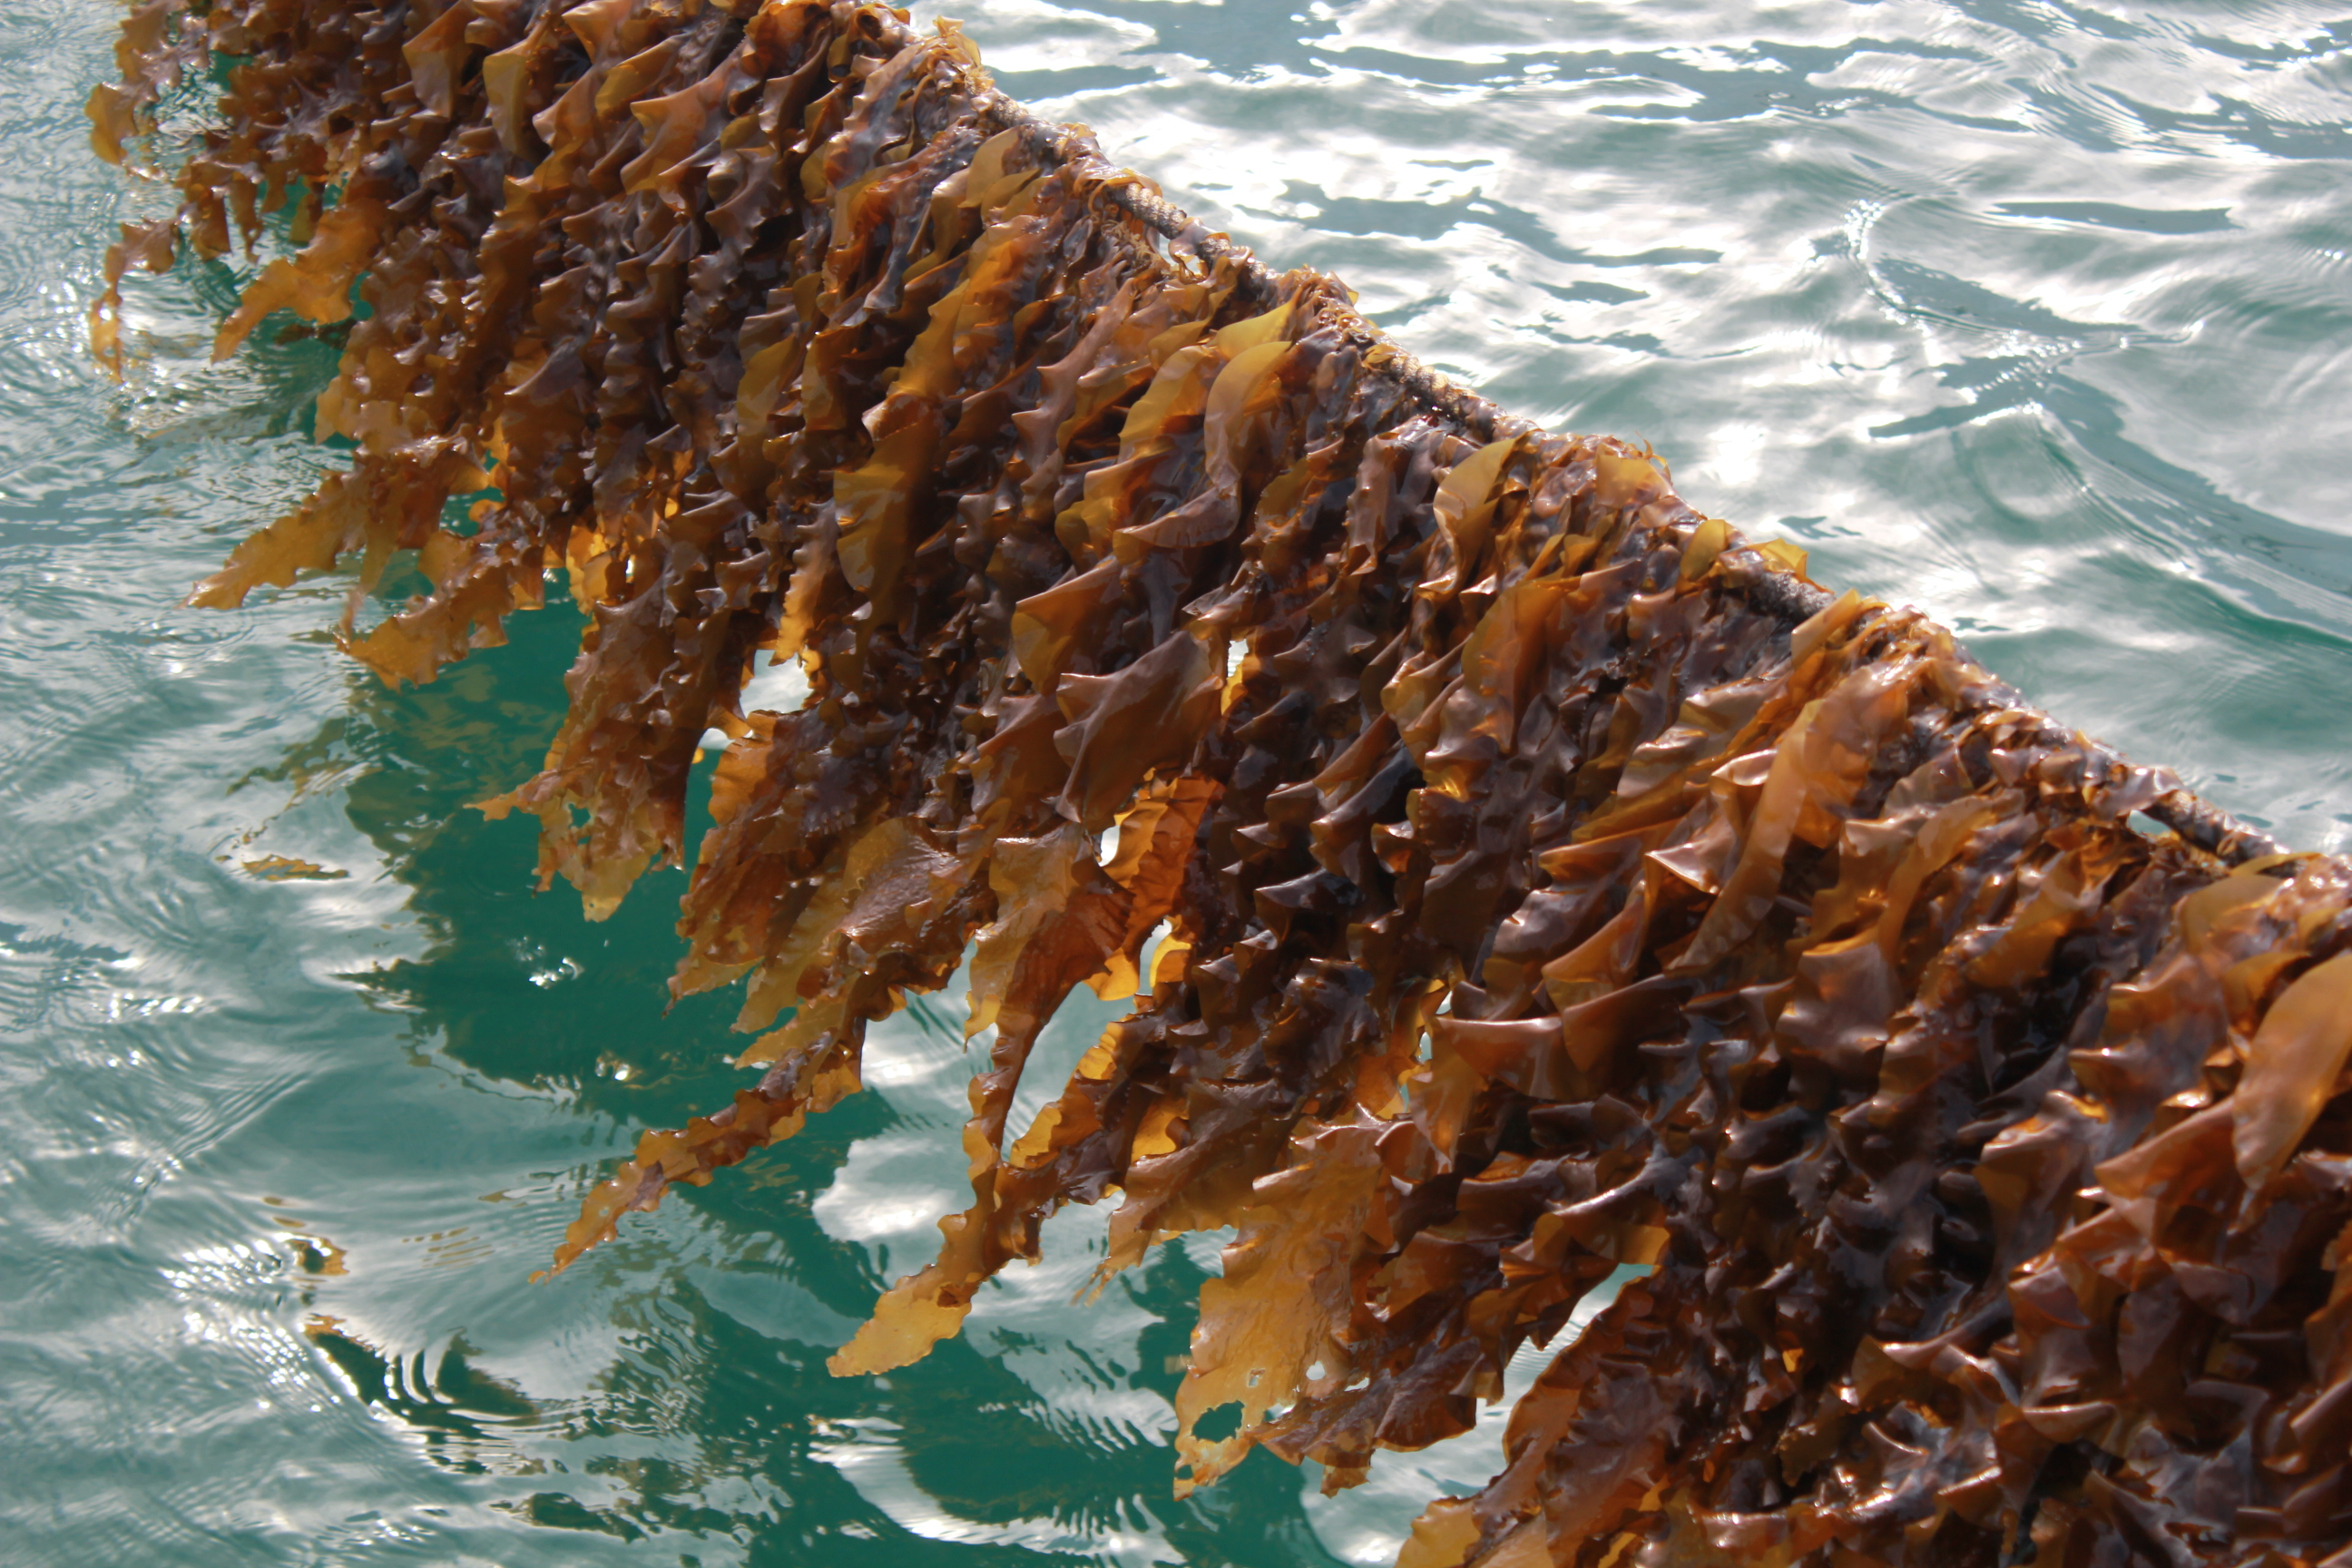
\includegraphics[width=\textwidth]{kelp_photo/kelp_photo1}
%DIFDELCMD <   %%%
\DIFdelendFL \DIFaddbeginFL \includegraphics[width=0.5\textwidth]{kelp_photo/sonja}
  \DIFaddendFL \caption{\DIFdelbeginFL \textit{\DIFdelFL{Saccharina Latissima}} %DIFAUXCMD
\DIFdelendFL \DIFaddbeginFL \textit{\DIFaddFL{Saccharina latissima}} \DIFaddendFL being harvested}
\end{figure}


\section{Background on Kelp Models}

Mathematical modeling of macroalgae growth is not a new topic, although it is a reemerging one.
Several authors in the second half of the twentieth century were interested in describing the growth and composition of the macroalgae \textit{Macrocystis pyrifera}, commonly known as ``giant kelp,'' which grows prolifically off the coast of southern California.
The first such mathematical model was developed by W.J. North for the Kelp Habitat Improvement Project at the California Institute of Technology in 1968 using seven variables.
By 1974, Nick Anderson greatly expanded on North's work, and created the first comprehensive model of kelp growth which he programmed using FORTRAN\cite{anderson_mathematical_1974}.
In his model, he accounts for solar radiation intensity as a function of time of year and time of day, and refraction on the surface of the water.
He uses a simple model for shading, simply specifying a single parameter which determines the percentage of light \DIFdelbegin \DIFdel{which }\DIFdelend \DIFaddbegin \DIFadd{that }\DIFaddend is allowed to pass through the kelp canopy floating on the surface of the water.
He also accounts for attenuation due to turbidity using Beer's Law.
Using this data on the availability of light, he calculates the photosynthesis rates and the growth experienced by the kelp.
\DIFdelbegin %DIFDELCMD < \\[-0.75em]
%DIFDELCMD < %%%
\DIFdelend 

Over a decade later in 1987, G.A.
Jackson expanded on Anderson's model for \textit{Macrocystis pyrifera}, with an emphasis on including more environmental parameters and a more complete description of the growth and decay of the kelp\cite{jackson_modelling_1987}. 
\DIFdelbegin \DIFdel{He }\DIFdelend \DIFaddbegin \DIFadd{The author }\DIFaddend takes into account respiration, frond decay, and \DIFdelbegin \DIFdel{most importantly for my work, }\DIFdelend sub-canopy light attenuation due to self-shading.
\DIFdelbegin \DIFdel{He simply adds a coefficient to the exponential decay of light as a function of depth to represent shading from kelp fronds.
He doesn't consider and radial nor }\DIFdelend \DIFaddbegin \DIFadd{Light attenuation is represented with a simple exponential model, and self-shading appears as an added term in the decay coefficient.
The author does not consider radial or }\DIFaddend angular dependence on shading. 
Jackson also expands Anderson's definition of canopy shading, treating the canopy not as a single layer, but as 0, 1, or 2 discrete layers, each composed of individual fronds.
While this is a significant improvement over Anderson's light model, it is still rather simplistic.
\DIFdelbegin %DIFDELCMD < \\[-0.75em]
%DIFDELCMD < %%%
\DIFdelend 

Both Anderson's and Jackson's model were carried out by numerically solving a system of differential equations over small time intervals.
In 1990, M.A. Burgman and V.A. Gerard developed a stochastic population model\cite{burgman_stage-structured_1990}.
This approach is quite different, and functions by dividing kelp plants into groups based on size and age \DIFdelbegin \DIFdel{, }\DIFdelend and generating random numbers to determine how the population distribution over these groups changes over time \DIFdelbegin \DIFdel{, }\DIFdelend based on measured rates of growth, death, decay, light availability, etc.
\DIFdelbegin \DIFdel{That }\DIFdelend \DIFaddbegin \DIFadd{In the }\DIFaddend same year, Nyman et. al. \DIFdelbegin \DIFdel{tested }\DIFdelend \DIFaddbegin \DIFadd{published }\DIFaddend a similar model \DIFdelbegin \DIFdel{in New Zealand, as well as }\DIFdelend \DIFaddbegin \DIFadd{alongside }\DIFaddend a Markov chain model, and compared the results with experimental data \DIFdelbegin \DIFdel{\mbox{%DIFAUXCMD
\cite{nyman_macrocystis_1990}}\hspace{0pt}%DIFAUXCMD
. }%DIFDELCMD < \\[-0.75em]
%DIFDELCMD < %%%
\DIFdelend \DIFaddbegin \DIFadd{collected in New Zealand\mbox{%DIFAUXCMD
\cite{nyman_macrocystis_1990}}\hspace{0pt}%DIFAUXCMD
.
}\DIFaddend 

In 1996 and 1998 respectively, P. Duarte and J.G. Ferreira used the size-class approach to create a more general model of macroalgae growth, and Yoshimori et. al. created a differential equation model of \textit{Laminaria religiosa} with specific emphasis on temperature dependence of growth rate\cite{duarte_model_1997,yoshimori_mathematical_1998}.
These were the some of the first models of kelp growth that did not specifically relate to \textit{Macrocystis pyrifera} (``giant kelp''). 
Initially, there was a great deal of excitement about this species due to it's incredible size and growth rate, but difficulties in harvesting and negative environmental impacts have caused scientists to investigate other kelp species. 
\DIFdelbegin %DIFDELCMD < \\[-0.75em]
%DIFDELCMD < %%%
\DIFdelend 

\section{Background on Radiative Transfer}
In terms of optical quantities, \DIFdelbegin \DIFdel{our }\DIFdelend \DIFaddbegin \DIFadd{of }\DIFaddend primary interest is in the radiance at each point from all directions, which affects the photosynthetic rate of the kelp, and therefore the total amount of biomass producible in a given area as well as the total nutrient remediation potential.
The equation governing the radiance throughout the system is known as the \DIFdelbegin \DIFdel{Radiative Transfer Equation }\DIFdelend \DIFaddbegin \DIFadd{radiative transfer equation }\DIFaddend (RTE), which has been largely unutilized in the fields of oceanography and aquaculture.
\DIFdelbegin \DIFdel{Meanwhile, it has been studied extensively in two fields: stellar astrophysicsand computer graphics}\DIFdelend \DIFaddbegin \DIFadd{The radiative transfer equation has been used primarily in stellar astrophysics; it's application to marine biology is fairly recent\mbox{%DIFAUXCMD
\cite{mobley_radiative_2001}}\hspace{0pt}%DIFAUXCMD
}\DIFaddend .
In its full form, radiance is a function of 3 spatial dimensions, 2 angular dimensions, and frequency, making for an incredibly complex problem. 
In this work, frequency is ignored, only monochromatic radiation is considered.
The RTE states that along a given path, radiance is decreased by absorption and scattering out of the path, while it is increased by emission and scattering into the path.
In our situation, emission is negligible, owing only perhaps to some small luminescent phytoplankton or \DIFdelbegin \DIFdel{some such }\DIFdelend \DIFaddbegin \DIFadd{other }\DIFaddend anomaly, and can therefore be safely ignored.

\DIFdelbegin \DIFdel{We use monochromatic radiative transfer in order to model the light field in an aqueous environment populated by vegetation.
The vegetation (kelp) is modeled by a spatial probability distribution, which we assume to be given.
The two quantities we seek to compute are }\textit{\DIFdel{radiance}} %DIFAUXCMD
\DIFdel{and }\textit{\DIFdel{irradiance}}%DIFAUXCMD
\DIFdel{.
Radiance is the intensity of light in at a particular point in a particular direction, while irradiance is the total light intensity at a point in space, integrated over all angles.
The Radiative Transfer Equation is an integro-partial differential equation for radiance, which has been used primarily in stellar astrophysics; it's application to marine biology is fairly recent \mbox{%DIFAUXCMD
\cite{mobley_radiative_2001}}\hspace{0pt}%DIFAUXCMD
.
}%DIFDELCMD < 

%DIFDELCMD < %%%
\DIFdelend Understanding the growth rate and nutrient recovery by
kelp cultures has important marine biological implications. For example, recent
work by our research group at Clarkson University, the University of Maine, and
SINTEF Fisheries and Aquaculture is investigating kelp aquaculture as a means to
recover nutrients from wastewater effluent plumes in coastal environments into a
valuable biomass feedstock for many products. Current models for kelp growth
place little emphasis on the way in which nearby plants shade one another.
Self-shading may be a significant model feature, though, as light availability
may impact the growth and composition of the kelp biomass, and thus the mixture
of goods that may be derived.

\section{Overview of Thesis}
The remainder of this document is organized as follows.
In Chapter \ref{chap:kelp}, \DIFdelbegin \DIFdel{we develop a probabilistic model }\DIFdelend \DIFaddbegin \DIFadd{probabilistic model is developed }\DIFaddend to describe the spatial distribution of kelp by assuming simple distributions for the lengths and orientations of fronds.
\DIFdelbegin \DIFdel{We begin Chapter \ref{chap:light} }\DIFdelend \DIFaddbegin \DIFadd{Chapter \ref{chap:light} begins }\DIFaddend with a survey of fundamental radiometric quantities and optical properties of matter.
\DIFdelbegin \DIFdel{We use the }\DIFdelend \DIFaddbegin \DIFadd{The }\DIFaddend spatial kelp distribution from Chapter \ref{chap:kelp} \DIFaddbegin \DIFadd{is used }\DIFaddend to determine optical properties of the combined water-kelp medium\DIFdelbegin \DIFdel{.
We then present the Radiative Transfer Equation}\DIFdelend \DIFaddbegin \DIFadd{,
and the radiative transfer equation}\DIFaddend , an integro-partial differential equation which describes the the light field as a function of position and angle\DIFaddbegin \DIFadd{, is discussed}\DIFaddend .
An asymptotic expansion is explored for cases where absorption dominates scattering in the medium, such as in very clear water or high kelp density.
In Chapter \ref{chap:numerical}, details are given for the numerical solution of the equations from Chapters \ref{chap:kelp} and \ref{chap:light}.
Both the full finite difference solution and the asymptotic approximation are described.
Next, in Chapter \ref{chap:parameters}, \DIFdelbegin \DIFdel{we discuss }\DIFdelend the availability of necessary parameters in the literature \DIFaddbegin \DIFadd{is discussed}\DIFaddend .
For those which are not readily available, \DIFdelbegin \DIFdel{we }\DIFdelend give rough estimates \DIFdelbegin \DIFdel{and briefly }\DIFdelend \DIFaddbegin \DIFadd{are given or }\DIFaddend describe experimental methods for their determination \DIFaddbegin \DIFadd{are described}\DIFaddend .
Then, in Chapter \ref{chap:model_analysis}, \DIFdelbegin \DIFdel{we investigate the }\DIFdelend necessary grid resolution for adequate accuracy in the full finite difference solution \DIFdelbegin \DIFdel{and compare }\DIFdelend \DIFaddbegin \DIFadd{is determined.
The finite difference solution is compared }\DIFaddend to the asymptotic approximation for a few \DIFdelbegin \DIFdel{parameter sets }\DIFdelend \DIFaddbegin \DIFadd{sets of optical properties}\DIFaddend .
Further, we \DIFdelbegin \DIFdel{determine }\DIFdelend \DIFaddbegin \DIFadd{showcase }\DIFaddend the effect of varying a few key parameters on the light field predicted by the asymptotic approximation.
Afterwards, \DIFdelbegin \DIFdel{we use }\DIFdelend the light model developed here \DIFdelbegin \DIFdel{in a full lifecycle }\DIFdelend \DIFaddbegin \DIFadd{is used in a numerical }\DIFaddend simulation of kelp growth\DIFdelbegin \DIFdel{and compare the }\DIFdelend \DIFaddbegin \DIFadd{, and the predicted }\DIFaddend light field and biomass production \DIFaddbegin \DIFadd{are compared }\DIFaddend to those predicted by a simpler 1D exponential decay light model.
Finally, \DIFdelbegin \DIFdel{we conclude with Chapter \ref{chap:conclusion} }\DIFdelend \DIFaddbegin \DIFadd{Chapter \ref{chap:conclusion} concludes the thesis }\DIFaddend by giving a brief summary of the model, discuss and its performance, and suggest improvements and avenues for future work.
 \chapter{KELP MODEL}
\label{chap:kelp}

In order to properly model the spatial distribution of light around the kelp, it is first necessary to formulate a spatial description of the kelp, which we do in this chapter.
We take a probabilistic approach to describing the kelp.
We begin by describing the distribution of kelp fronds, and through algebraic manipulation, we are able to assign to each point in space a probability that kelp occupies the location.

\section{Physical Setup}
\DIFdelbegin \DIFdel{Being a salt water species, macroalgae cultivation occurs primarily in the ocean, with the exception of the initial stage of growth, }\DIFdelend \DIFaddbegin \DIFadd{The life of cultivated macroalgae generally begins in the laboratory, }\DIFaddend where microscopic kelp spores are inoculated onto a thread in a small laboratory pool. 
This thread is \DIFdelbegin \DIFdel{then }\DIFdelend wrapped around a large rope, which is placed in the ocean and generally suspended by buoys in one of two configurations: horizontal or vertical.
\DIFdelbegin \DIFdel{Thus far, I am primarily concerned with modeling the vertical rope case, in which the kelp plants extend radially outward from the rope in all directions, which are made up }\DIFdelend \DIFaddbegin \DIFadd{We consider only the case of a rigid vertical rope which does not sway in the current.
The mature }\textit{\DIFadd{Saccharina latissima}} \DIFadd{plant consists }\DIFaddend of a single frond (leaf), \DIFaddbegin \DIFadd{a }\DIFaddend stipe (stem) and \DIFaddbegin \DIFadd{a }\DIFaddend holdfast (root structure).
\DIFdelbegin \DIFdel{We consider a rectangular grid of such vertical ropes. 
Plants extending from each rope will shade both themselves and their neighbors
to varying degrees based on the depth of the kelp, the rope spacing, the angle
of incident light on the surface and the nature of scattering in the water .
In addition, light will be naturally absorbed by the water to varying degrees as determined by the clarity of the water}\DIFdelend \DIFaddbegin \DIFadd{For the sake of this model, only the kelp frond is considered, and its base is attached directly to the rope.
The ``gentle undulation approximation'' is employed, whereby it is assumed that fronds are perfectly horizontal.
While on at any point in time they may point up or down due to water current and gravity, we consider the horizontal
state to be an average configuration.
This simplifaction allows for the three-dimensionally distributed population of kelp fronds
to be considered a collection of independent populations in two-dimensional depth layers}\DIFaddend .

\begin{figure}[H]
	\centering
	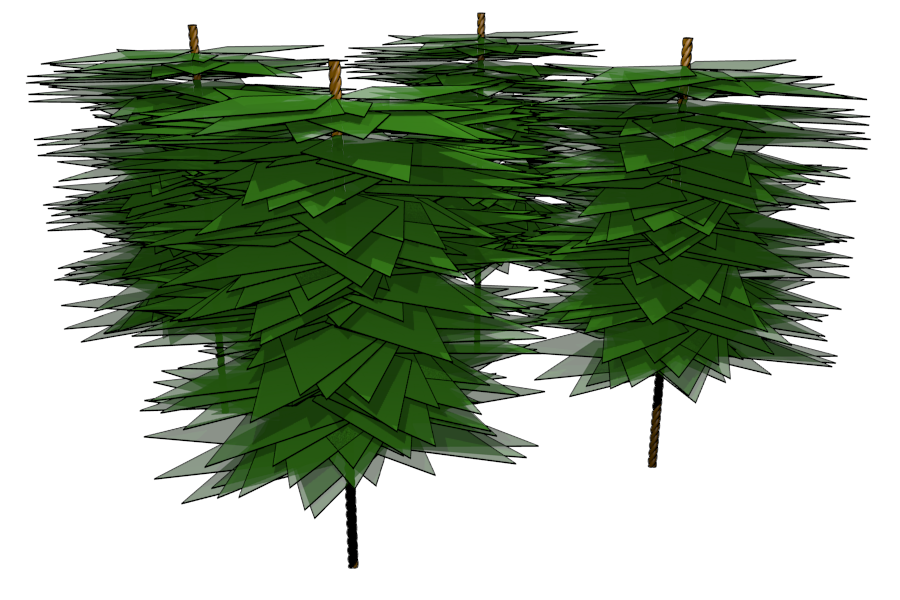
\includegraphics[width=3.5in]{kelp_array}
	\DIFdelbeginFL %DIFDELCMD < \captionof{figure}{$4\times 4$ array of vertical kelp ropes}
%DIFDELCMD < %%%
\DIFdelendFL \DIFaddbeginFL \captionof{figure}{Rendering of four nearby vertical kelp ropes}
\DIFaddendFL \end{figure}
\DIFdelbegin \section{\DIFdel{Coordinate System}}
%DIFAUXCMD
\addtocounter{section}{-1}%DIFAUXCMD
\DIFdelend 

\DIFaddbegin \section{\DIFadd{Coordinate System}}
\DIFaddend Consider the rectangular domain
\begin{align*}
  \xmin &\leq x \leq \xmax, \\
  \ymin &\leq y \leq \ymax, \\
  \zmin &\leq z \leq \zmax.
\end{align*}
For all three dimensional analysis, we use the absolute coordinate system defined in \DIFdelbegin \DIFdel{figure }\DIFdelend \DIFaddbegin \DIFadd{Figure }\DIFaddend \ref{fig:3dcoords}.
In the following sections, it is necessary to convert between Cartesian and spherical coordinates, which we do using the relations
\DIFdelbegin \begin{align*}
	\DIFdel{\begin{split}
		x & = r\sin\phi\cos\theta, \\
		y & = r\sin\phi\sin\theta, \\
		z & = r\cos\phi. \\
	%DIFDELCMD < \label{eqn:coords}%%%
	\end{split}
}\end{align*}
%DIFAUXCMD
\DIFdelend \DIFaddbegin \begin{equation}
  \DIFadd{\left\{
	\begin{split}
		x & = r\sin\phi\cos\theta, \\
		y & = r\sin\phi\sin\theta, \\
		z & = r\cos\phi. \\
	\end{split}
  \right.
	\label{eqn:coords}
}\end{equation}
\DIFaddend 

Therefore, for some function $f(x,y,z)$, we can write its derivative along a path in spherical coordinates in terms of Cartesian coordinates using the chain rule.
\DIFdelbegin \begin{displaymath}
	\DIFdel{\frac{\partial f}{\partial r} 
	=\frac{\partial f}{\partial x}\frac{\partial x}{\partial r} 
	+ \frac{\partial f}{\partial y}\frac{\partial y}{\partial r} 
	+ \frac{\partial f}{\partial z}\frac{\partial z}{\partial r}
}\end{displaymath}
%DIFAUXCMD
\DIFdelend \DIFaddbegin \begin{equation*}
	\DIFadd{\frac{\partial f}{\partial r} 
	=\frac{\partial f}{\partial x}\frac{\partial x}{\partial r} 
	+ \frac{\partial f}{\partial y}\frac{\partial y}{\partial r} 
	+ \frac{\partial f}{\partial z}\frac{\partial z}{\partial r}
}\end{equation*}
\DIFaddend Then, calculating derivatives from \eqref{eqn:coords} yields
\begin{equation}
	\frac{\partial f}{\partial r} 
	=\frac{\partial f}{\partial x}\sin\phi\cos\theta
	+ \frac{\partial f}{\partial y}\sin\phi\sin\theta
	+ \frac{\partial f}{\partial z}\cos\phi.
	\label{eqn:partials}
\end{equation}
\begin{figure}[H]
	\centering
	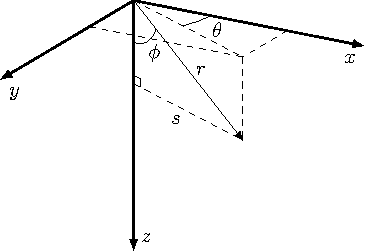
\includegraphics[width=3in]{3d_coords}
	\caption{Downward-facing right-handed coordinate system with radial distance $r$ from the origin, distance $s$ from the $z$ axis, zenith angle $\phi$ and azimuthal angle $\theta$}
	\label{fig:3dcoords}
\end{figure}


\section{Population Distributions}
\DIFaddbegin \DIFadd{In order to construct a spatial distribution of kelp fronds, a simple kite-shaped geometry is introduced,
and frond lengths and azimuthal orientations are assumed to be distributed predictably.
It is assumed that fronds extend perfectly horizontally 
}\DIFaddend 

\subsection{Frond Shape}
\label{sec:shape}

\begin{figure}[h]
	\centering
  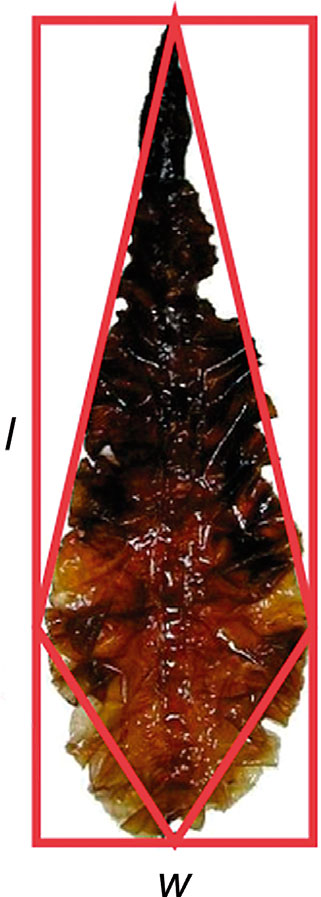
\includegraphics[width=1.2in]{kelp_photo/kite}
  \qquad
	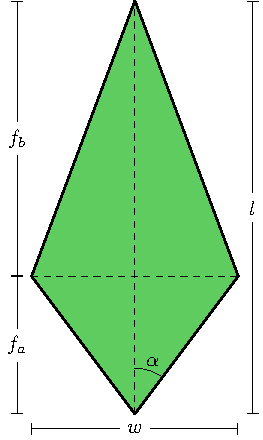
\includegraphics[width=2in]{frond}
	\captionof{figure}{Simplified kite-shaped frond}
	\label{fig:frond}
\end{figure}

\DIFdelbegin \DIFdel{We assume the frond is a kite }\DIFdelend \DIFaddbegin \DIFadd{The frond is assumed to be kite-shaped }\DIFaddend with length $l$ from base to tip, and width $w$ from left to right.
\DIFdelbegin \DIFdel{The }\DIFdelend \DIFaddbegin \DIFadd{In Figure \ref{fig:frond}, the base is shown at the bottom and the tip is shown at the top.
The proximal length is the }\DIFaddend shortest distance from the base to the diagonal connecting the left and right corners\DIFdelbegin \DIFdel{is called }\DIFdelend \DIFaddbegin \DIFadd{, and is notated as }\DIFaddend $f_a$\DIFdelbegin \DIFdel{, and the }\DIFdelend \DIFaddbegin \DIFadd{.
Likewise, the distal length is the }\DIFaddend shortest distance from that diagonal to the tip\DIFdelbegin \DIFdel{is called }\DIFdelend \DIFaddbegin \DIFadd{, notated }\DIFaddend $f_b$.
 We have
 \DIFdelbegin \begin{displaymath}
	 \DIFdel{f_a + f_b = l
 }\end{displaymath}
%DIFAUXCMD
\DIFdelend \DIFaddbegin \begin{equation*}
	 \DIFadd{f_a + f_b = l
 }\end{equation*}
\DIFaddend When considering a whole population with varying sizes, it is more convenient to specify ratios than absolute lengths.
Let the following ratios be defined.
\DIFdelbegin \begin{align*}
	\DIFdel{f_r }&\DIFdel{= \frac{l}{w} }\\
	\DIFdel{f_s }&\DIFdel{= \frac{f_a}{f_b}
}\end{align*}
%DIFAUXCMD
\DIFdelend \DIFaddbegin \begin{align*}
	\DIFadd{f_r }&\DIFadd{= \frac{l}{w} }\\
	\DIFadd{f_s }&\DIFadd{= \frac{f_a}{f_b}
}\end{align*}
\DIFaddend These ratios are assumed to be consistent among the entire population, making all fronds geometrically similar.
With these definitions, the shape of the frond can be fully specified by $l$, $f_r$, and $f_s$.
It is possible, then, to redefine $w$, $f_a$ and $f_b$ as follows from the preceding formulas.

\DIFdelbegin \begin{align*}
	\DIFdel{w }&\DIFdel{= \frac{l}{f_r} }\\
	\DIFdel{f_a }&\DIFdel{= \frac{lf_s}{1+f_s} }\\
	\DIFdel{f_b }&\DIFdel{= \frac{l}{1+f_s}
}\end{align*}
%DIFAUXCMD
\DIFdelend \DIFaddbegin \begin{align*}
	\DIFadd{w }&\DIFadd{= \frac{l}{f_r} }\\
	\DIFadd{f_a }&\DIFadd{= \frac{lf_s}{1+f_s} }\\
	\DIFadd{f_b }&\DIFadd{= \frac{l}{1+f_s}
}\end{align*}
\DIFaddend 

The angle $\alpha$, half of the angle at the base corner, is also \DIFdelbegin \DIFdel{important in our analysis}\DIFdelend \DIFaddbegin \DIFadd{noteworthy}\DIFaddend .
Using the above equations,
\DIFdelbegin \begin{displaymath}
	\DIFdel{\alpha = \tan^{-1}\left(\frac{2f_rf_s}{1+f_s}\right)
}\end{displaymath}
%DIFAUXCMD
\DIFdelend \DIFaddbegin \begin{equation*}
	\DIFadd{\alpha = \tan^{-1}\left(\frac{2f_rf_s}{1+f_s}\right)
}\end{equation*}
\DIFaddend 

The area of the frond is given by
\DIFdelbegin \begin{displaymath}
  \DIFdel{A = \frac{lw}{2} = \frac{l^2}{2f_r}.
}\end{displaymath}
%DIFAUXCMD
\DIFdelend \DIFaddbegin \begin{equation*}
  \DIFadd{A = \frac{lw}{2} = \frac{l^2}{2f_r}.
}\end{equation*}
\DIFaddend 

Likewise, if the area is known, then the length is
\begin{equation}
  l = \sqrt{2Af_r}\DIFaddbegin \DIFadd{.
  }\DIFaddend \label{eqn:length-from-area}
\end{equation}

\subsection{Length and Angle Distributions}
\label{sec:dist}
\DIFdelbegin \DIFdel{We assume that frond lengths are }\DIFdelend \DIFaddbegin \DIFadd{Frond lengths are assumed to be }\DIFaddend normally distributed with mean $\mu_l$ and standard deviation $\sigma_l$.
\DIFdelbegin \DIFdel{We assume the frond }\DIFdelend \DIFaddbegin \DIFadd{That is, the frond length distribution has the probability density function (PDF)
}\begin{equation*}
  \DIFadd{P_l(l) = \frac{1}{\sqrt{2\pi\sigma_l^2}}\exp\left(\frac{(l-\mu_l)^2}{2\sigma_l^2}\right).
}\end{equation*}

\DIFadd{It is further assumed that frond }\DIFaddend angle varies according to the von Mises distribution, which is the periodic analogue of the normal distribution, defined on $[-\pi,\pi]$ rather than $(-\infty,\infty)$.
The von Mises distribution has two parameters, $\mu$ and $\kappa$, which shift and sharpen its peak respectively, as shown in Figure \ref{fig:vonmises}.
$\kappa$ can be considered analogous to $1/\sigma$ in the normal distribution.
\DIFdelbegin \DIFdel{Here, we use $\mu = \theta_w$ and $\kappa = v_w$.
}\DIFdelend That is, in the case of zero current velocity, the frond angles are be distributed uniformly, while as current velocity increases, they become increasingly likely to be pointing in the direction of the current\DIFdelbegin \DIFdel{.
}\DIFdelend \DIFaddbegin \DIFadd{, depending on the stiffness of the frond.
Assuming a linear relationship between the current velocity and the steepness of the angular distribution, define the frond bending coefficient $\eta$, with units \mbox{%DIFAUXCMD
\SI{}{\s\per\m}}\hspace{0pt}%DIFAUXCMD
.
Then, in use $\mu = \theta_w$ and $\kappa = \eta v_w$ as the von Mises distribution parameters.
}\DIFaddend Note that $\theta_w$ and $v_w$ vary over depth\DIFdelbegin \DIFdel{.
}%DIFDELCMD < 

%DIFDELCMD < %%%
\DIFdel{The PDF for this distribution is
}\begin{displaymath}
	\DIFdel{P_{\theta_f}(\theta_f) = \frac{\exp\left(v_w\cos(\theta_f-v_w)\right)}{2\pi I_0(v_w)}
}\end{displaymath}
%DIFAUXCMD
\DIFdelend \DIFaddbegin \DIFadd{, while $\eta$ is assumed constant for the population.
Then, the PDF for the von Mises frond angle distribution is
}\begin{equation*}
	\DIFadd{P_{\theta_f}(\theta_f) = \frac{\exp\left(\eta v_w\cos(\theta_f-\theta_w)\right)}{2\pi I_0(\eta v_w)},
}\end{equation*}
\DIFaddend where $I_0(x)$ is the modified Bessel function of the first kind of order 0.
Notice that unlike the normal distribution, the von Mises distribution approaches a \textit{non-zero} uniform distribution as $\kappa$ approaches \DIFdelbegin \DIFdel{0.
}\begin{displaymath}
	\DIFdel{\displaystyle \lim_{v_w \to 0}P_{\theta_f}(\theta_f) = \frac{1}{2\pi} \;\forall\, \theta_f \in }[\DIFdel{-\pi,\pi}]
\end{displaymath}
%DIFAUXCMD
\DIFdelend \DIFaddbegin \DIFadd{0, so
}\begin{equation*}
	\DIFadd{\displaystyle \lim_{v_w \to 0}P_{\theta_f}(\theta_f) = \frac{1}{2\pi} \;\forall\, \theta_f \in }[\DIFadd{-\pi,\pi}]\DIFadd{.
}\end{equation*}
\DIFaddend 

\begin{figure}[h]
	\centering
	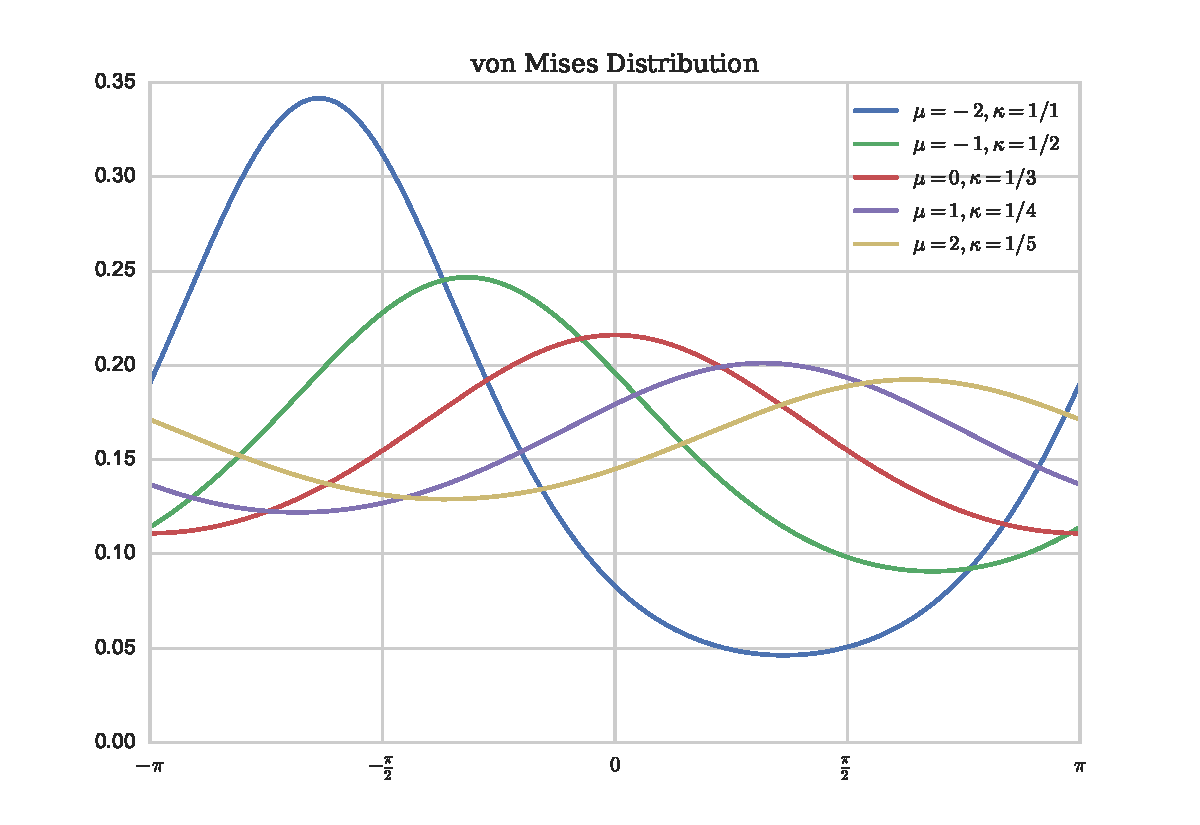
\includegraphics[width=.75\linewidth]{vonmises_2}
	\captionof{figure}{von Mises distribution for a variety of parameters}
	\label{fig:vonmises}
\end{figure}

\subsection{Joint Length-Orientation Distribution}
\DIFdelbegin %DIFDELCMD < \label{sec:2d_dist}
%DIFDELCMD < %%%
\DIFdelend \DIFaddbegin \label{sec:dist_2d}
\DIFaddend The previous two distributions can reasonably be assumed to be independent of one another. That is, the angle of the frond does not depend on the length, or vice versa.
Therefore, the probability of a frond simultaneously having a given frond length and angle is the product of their individual probabilities.

Given independent events $A$ and $B$,
\DIFdelbegin \begin{displaymath}
	\DIFdel{\label{eq:ind_prob}
	P(A \cap B) = P(A)P(B)
}\end{displaymath}
%DIFAUXCMD
\DIFdelend \DIFaddbegin \begin{equation*}
	\DIFadd{\label{eq:ind_prob}
	P(A \cap B) = P(A)P(B)
}\end{equation*}
\DIFaddend Then the probability of frond length $l$ and frond angle $\theta_f$ coinciding is 
\DIFdelbegin \begin{displaymath}
	\DIFdel{P_{2D}(\theta_f,l) = P_{\theta_f}(\theta_f) \cdot L(l)
}\end{displaymath}
%DIFAUXCMD
\DIFdelend \DIFaddbegin \begin{equation*}
	\DIFadd{P_{2D}(\theta_f,l) = P_{\theta_f}(\theta_f) \cdot P_l(l)
}\end{equation*}
\DIFaddend A contour plot of this 2D distribution for a specific set of parameters is shown in \DIFdelbegin \DIFdel{figure }\DIFdelend \DIFaddbegin \DIFadd{Figure }\DIFaddend \ref{fig:dist_2d}, where probability is represented by color in the 2D plane.
Darker green represents higher probability, while lighter beige represents lower probability.
In \DIFdelbegin \DIFdel{figure }\DIFdelend \DIFaddbegin \DIFadd{Figure }\DIFaddend \ref{fig:kelp_sample}, 50 samples are drawn from this distribution and plotted.

It is important to note that if $P_{\theta_f}$ were dependent on $l$, the above definition of $P_{2D}$ would no longer be valid.
For example, it might be more realistic to say that larger fronds are less likely to bend towards the direction of the current.
In this case, \eqref{eq:ind_prob} would no longer hold, and it would be necessary to use the \DIFdelbegin \DIFdel{following }\DIFdelend more general relation
\DIFdelbegin \DIFdel{.
}\begin{displaymath}
	\DIFdel{P(A \cap B) = P(A)P(B|A) = P(B)P(B|A)
}\end{displaymath}
%DIFAUXCMD
\DIFdel{This }\DIFdelend \DIFaddbegin \begin{equation*}
	\DIFadd{P(A \cap B) = P(A)P(B|A) = P(B)P(B|A),
}\end{equation*}
\DIFadd{which }\DIFaddend is currently not taken into consideration in this model.

\begin{figure}[h]
	\centering
	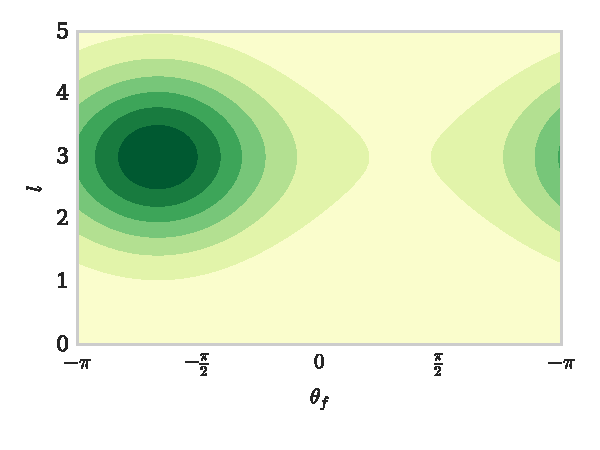
\includegraphics[width=.75\linewidth]{prob_2d}
	\vspace{-3em}
	\captionof{figure}{2D length-angle probability distribution with $\theta_w=2\pi/3,v_w=1$}
	\label{fig:dist_2d}
\end{figure}

\begin{figure}[h]
	\centering
	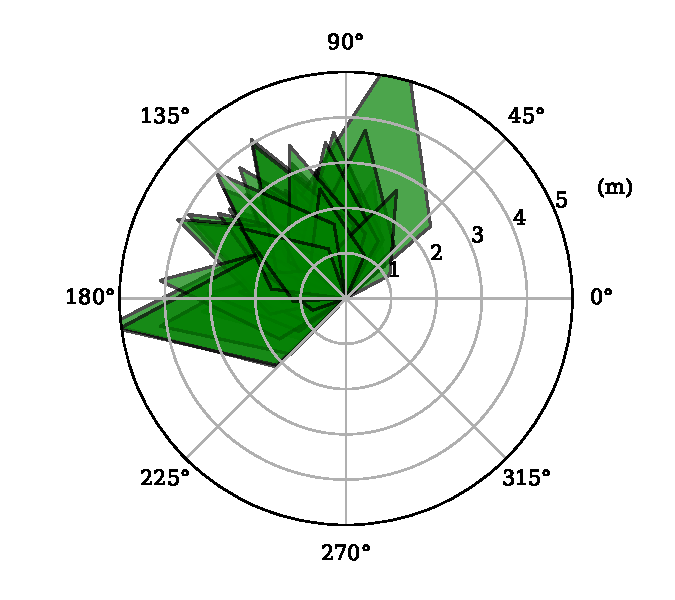
\includegraphics[width=.75\linewidth]{kelp_sample}
	\vspace{-2em}
	\captionof{figure}{A sample of 50 kelp fronds with length and angle picked from the distribution above with $f_s=0.5$ and $f_r=2$.}
	\label{fig:kelp_sample}
\end{figure}

\section{Spatial Distribution}
\subsection{Rotated Coordinate System}
\label{sec:rot_coords}
To determine under what conditions a frond will occupy a given point, we begin by
describing the shape of the frond in Cartesian \DIFdelbegin \DIFdel{and then converting }\DIFdelend \DIFaddbegin \DIFadd{coordinates and then convert }\DIFaddend to polar coordinates.
Of primary interest are the edges connected to the frond tip.
For convenience, we will use a rotated coordinate system $(\theta',s)$ such that the line connecting the base to the tip is vertical, with the base at $(0,0)$.
\DIFdelbegin \DIFdel{The }\DIFdelend \DIFaddbegin \DIFadd{Denote the }\DIFaddend Cartesian analogue of this coordinate system \DIFdelbegin \DIFdel{, }\DIFdelend \DIFaddbegin \DIFadd{as }\DIFaddend $(x',y')$ \DIFdelbegin \DIFdel{, has the following properties.
}\begin{align*}
	\DIFdel{x' }&\DIFdel{= s\cos\theta' }\\ 
	\DIFdel{y' }&\DIFdel{= s\sin\theta'
}\end{align*}
%DIFAUXCMD
\DIFdel{and
}\begin{align*}
	\DIFdel{s }&\DIFdel{= \sqrt{x'^2+y'^2}
}\end{align*}
%DIFAUXCMD
%DIFDELCMD < \vspace{-1em}
%DIFDELCMD < %%%
\begin{align*}
	\DIFdel{\theta' }&\DIFdel{= \atantwo(y, x)
}\end{align*}
%DIFAUXCMD
\DIFdelend \DIFaddbegin \DIFadd{which is related to $(\theta',s)$ by
}\begin{align*}
	\DIFadd{x' }&\DIFadd{= s\cos\theta' }\\ 
	\DIFadd{y' }&\DIFadd{= s\sin\theta' }\\
	\DIFadd{s }&\DIFadd{= \sqrt{x'^2+y'^2}, }\\
	\DIFadd{\theta' }&\DIFadd{= \atantwo(y, x).
}\end{align*}
\DIFaddend 

\subsection{Functional Description of Frond Edge}
With this coordinate system established, \DIFdelbegin \DIFdel{we can describe }\DIFdelend the outer two edges of the frond \DIFaddbegin \DIFadd{can be described }\DIFaddend in Cartesian coordinates as a piecewise linear function connecting the left corner: $(-w/2,f_a)$, the tip: $(0,l)$, and the right corner: $(w/2,f_a)$.
This function has the form
\DIFdelbegin \begin{displaymath}
	\DIFdel{y'_f(x') = l-\sign(x')\frac{f_b}{w/2}x'.
}\end{displaymath}
%DIFAUXCMD
%DIFDELCMD < 

%DIFDELCMD < %%%
\DIFdelend \DIFaddbegin \begin{equation*}
	\DIFadd{y'_f(x') = l-\sign(x')\frac{f_b}{w/2}x'.
}\end{equation*}
\DIFaddend Using the equations in Section \ref{sec:rot_coords}, this can be written in polar coordinates after some rearrangement as
\DIFdelbegin \begin{displaymath}
	\DIFdel{s_f'(\theta') = \frac{l}{\sin\theta' + S(\theta')\frac{2f_b}{w}\cos\theta'}
}\end{displaymath}
%DIFAUXCMD
\DIFdel{where
}\begin{displaymath}
	\DIFdel{S(\theta') = \sign(\theta'-\pi/2)
}\end{displaymath}
%DIFAUXCMD
%DIFDELCMD < 

%DIFDELCMD < %%%
\DIFdelend \DIFaddbegin \begin{equation*}
	\DIFadd{s_f'(\theta') = \frac{l}{\sin\theta' + S(\theta')\frac{2f_b}{w}\cos\theta'},
}\end{equation*}
\DIFadd{where
}\begin{equation*}
	\DIFadd{S(\theta') = \sign(\theta'-\pi/2).
}\end{equation*}
\DIFaddend Then, using the relationships in Section \ref{sec:shape}, \DIFdelbegin \DIFdel{we can rewrite }\DIFdelend the above equation \DIFaddbegin \DIFadd{can be rewritten }\DIFaddend in terms of \DIFdelbegin \DIFdel{our }\DIFdelend \DIFaddbegin \DIFadd{the }\DIFaddend frond ratios $f_s$ and $f_r$ \DIFdelbegin \DIFdel{.
}\begin{displaymath}
	\DIFdel{\label{eq:rf_rel}
	s_f'(\theta') = \frac{l}{\sin\theta' + S(\theta')\frac{2f_r}{1+f_s}\cos\theta'}
}\end{displaymath}
%DIFAUXCMD
%DIFDELCMD < 

%DIFDELCMD < %%%
\subsection{\DIFdel{Absolute Coordinates}}
%DIFAUXCMD
\addtocounter{subsection}{-1}%DIFAUXCMD
%DIFDELCMD < \label{sec:abs_coords}
%DIFDELCMD < %%%
\DIFdelend \DIFaddbegin \DIFadd{as
}\begin{equation*}
	\DIFadd{\label{eq:rf_rel}
	s_f'(\theta') = \frac{l}{\sin\theta' + S(\theta')\frac{2f_r}{1+f_s}\cos\theta'}.
}\end{equation*}
\DIFaddend To generalize to a frond pointed at an angle $\theta_f$, we \DIFdelbegin \DIFdel{will use }\DIFdelend \DIFaddbegin \DIFadd{introduce }\DIFaddend the coordinate system $(\theta,s)$ such that
\DIFdelbegin \begin{displaymath}
	\DIFdel{\theta = \theta' + \theta_f - \frac{\pi}{2}
}\end{displaymath}
%DIFAUXCMD
\DIFdelend \DIFaddbegin \begin{equation*}
	\DIFadd{\theta = \theta' + \theta_f - \frac{\pi}{2}
}\end{equation*}
\DIFaddend Then, for a frond pointed at the arbitrary angle $\theta_f$, the function for the outer edges can be written as 
\DIFdelbegin \begin{displaymath}
	\DIFdel{\label{eq:rf_abs}
	s_f(\theta) = s_f'\left(\theta - \theta_f + \frac{\pi}{2} \right)
}\end{displaymath}
%DIFAUXCMD
\DIFdelend \DIFaddbegin \begin{equation*}
	\DIFadd{\label{eq:rf_abs}
	s_f(\theta) = s_f'\left(\theta - \theta_f + \frac{\pi}{2} \right).
}\end{equation*}
\DIFaddend 

\subsection{Conditions for Occupancy}
\DIFaddbegin \DIFadd{We now formulate the conditions under which a kite shape frond occupies a point
in the sense that the point lies within its interior.
Combining these conditions with the size and orientation distributions from \ref{sec:dist}
allows a spatial distribution of the kelp fronds to be calculated.
}

\DIFaddend Consider a fixed frond of length $l$ at an angle $\theta_f$. The point
$(\theta,s)$ is occupied by the frond if
\DIFdelbegin \begin{align*}
	\DIFdel{\left|\theta_f - \theta \right| < \alpha
	\shortintertext{and}
	s < s_f(\theta)
}\end{align*}
%DIFAUXCMD
\DIFdelend \DIFaddbegin \begin{align*}
	\DIFadd{\left|\theta_f - \theta \right| < \alpha,
	s < s_f(\theta).
}\end{align*}
\DIFaddend 

Equivalently, \DIFdelbegin \DIFdel{letting the }\DIFdelend \DIFaddbegin \DIFadd{the opposite perspective can be taken.
Letting the }\DIFaddend point $(\theta,s)$ be fixed, a frond occupies the point if
\DIFdelbegin \DIFdel{the following conditions are satisfied.
}\DIFdelend \begin{align}
	\theta - \alpha < \theta_f < \theta + \alpha\DIFaddbegin \DIFadd{,
	}\DIFaddend \label{eqn:rs_th} \DIFdelbegin %DIFDELCMD < \shortintertext{and}
%DIFDELCMD < 	%%%
\DIFdelend \DIFaddbegin \\
	\DIFaddend l > l_{min}(\theta,s)\DIFaddbegin \DIFadd{,
	}\DIFaddend \label{eqn:rs_l}
\end{align}
where
\DIFdelbegin \begin{displaymath}
	\DIFdel{l_{min}(\theta,s) = s \cdot \frac{l}{s_f(\theta)}
}\end{displaymath}
%DIFAUXCMD
%DIFDELCMD < 

%DIFDELCMD < %%%
\DIFdelend \DIFaddbegin \begin{equation*}
	\DIFadd{l_{min}(\theta,s) = s \cdot \frac{l}{s_f(\theta)}.
}\end{equation*}
\DIFaddend Then, considering the point to be fixed, \eqref{eqn:rs_th} and \eqref{eqn:rs_l} define the spacial region $R_s(\theta,s)$ called the ``occupancy region for $(\theta,s)$'' with the property that if the tip of a frond lies within this region (i.e.\DIFaddbegin \DIFadd{, }\DIFaddend $(\theta_f,l) \in R_s(\theta,s)$), then it occupies the point.
$R_s(3\pi/4,3/2)$ is shown in blue in \DIFdelbegin \DIFdel{figure }\DIFdelend \DIFaddbegin \DIFadd{Figure }\DIFaddend \ref{fig:shade_area} and the smallest possible occupying fronds for several values of $\theta_f$ are shown in various colors.
Any frond longer than these at the same angle will also occupy the point.

\begin{figure}[h]
	\centering
	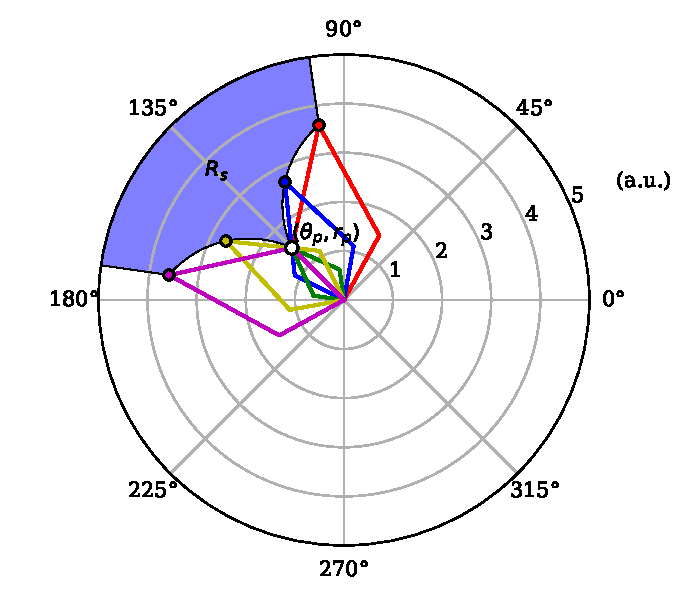
\includegraphics[width=.75\linewidth]{shade_area}
	\vspace{-2em}
	\captionof{figure}{Outlines of minimum-length fronds for a variety of angles to occupy the point $(\theta,s)=(3\pi/4,3/2)$}
	\label{fig:shade_area}
\end{figure}

\subsection{Probability of Occupancy}
We are interested in the probability that, given a fixed point $(\theta,s)$, values of $l$ and $\theta_f$ chosen from the distributions described in Section \ref{sec:dist} will fall in the occupancy region.
This is found by integrating $P_{2D}$ over the occupancy region for $(\theta,s)$\DIFdelbegin \DIFdel{, as depicted in figure \ref{fig:cart_shade}}\DIFdelend .

\begin{figure}[H]
	\centering
	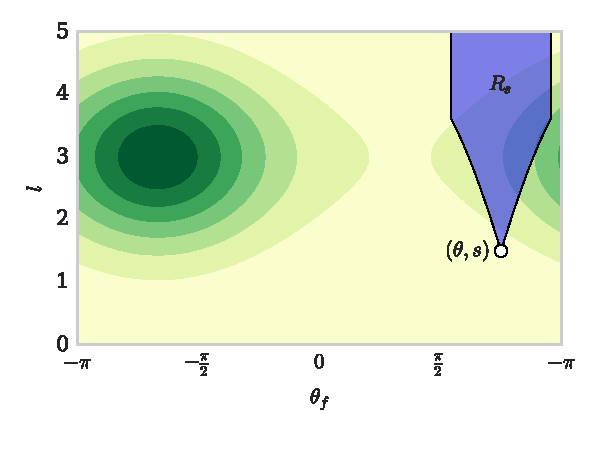
\includegraphics[width=.75\linewidth]{cart_shade}
	\vspace{-3em}
	\captionof{figure}{Contour plot of $P_{2D}(\theta_f,l)$ overlayed with the
    region in the $\theta_f-l$ plane which results in a frond occupying the point $(\theta,s)=(3\pi/4,3/2)$}
	\label{fig:cart_shade}
\end{figure}

\DIFdelbegin \DIFdel{Now, integrating }\DIFdelend \DIFaddbegin \DIFadd{Integrating }\DIFaddend $P_{2D}(\theta_f,l)$ over $R_s(\theta,s)$ \DIFaddbegin \DIFadd{as depicted in Figure \ref{fig:cart_shade} }\DIFaddend yields the proportion of the population occupying the point $(\theta,s)$\DIFdelbegin \DIFdel{.
}\begin{align*}
		\DIFdel{\tilde{P}_k(\theta,s,z)	}&\DIFdel{= \iint_{R_s(\theta,s)}
								P_{2D}(\theta_f,l)
								\,dl\,d\theta_f \nonumber }\\
							&\DIFdel{= \int_{\theta-\alpha}^{\theta+\alpha} 
								\int_{l_{min}(\theta_f)}^\infty
								P_{2D}(\theta_f,l)
								\,dl\,d\theta_f
}\end{align*}
%DIFAUXCMD
\DIFdelend \DIFaddbegin \DIFadd{,
}\begin{align*}
		\DIFadd{\tilde{P}_k(\theta,s,z)	}&\DIFadd{= \iint_{R_s(\theta,s)}
								P_{2D}(\theta_f,l)
								\,dl\,d\theta_f \nonumber }\\
							&\DIFadd{= \int_{\theta-\alpha}^{\theta+\alpha} 
								\int_{l_{min}(\theta_f)}^\infty
								P_{2D}(\theta_f,l)
								\,dl\,d\theta_f.
}\end{align*}
\DIFaddend 

Then, multiplying $\tilde{P}_k$ by the number of fronds in the population $n$ of the depth layer gives the expected number of fronds occupying the point.
\DIFdelbegin \DIFdel{Now, assuming }\DIFdelend \DIFaddbegin \DIFadd{Assuming }\DIFaddend a uniform thickness $t$ for all fronds, and a thickness $dz$ of the depth layer, \DIFdelbegin \DIFdel{we find }\DIFdelend the proportion of the grid cell occupied by kelp \DIFdelbegin \DIFdel{to be
}\begin{displaymath}
  \DIFdel{P_k = \frac{nt}{dz}\tilde{P}.
}\end{displaymath}
%DIFAUXCMD
\DIFdelend \DIFaddbegin \DIFadd{is found to be
}\begin{equation*}
  \DIFadd{P_k = \frac{nt}{dz}\tilde{P}_k.
}\end{equation*}
\DIFaddend 

Then, the effective absorption coefficient can be calculated at any point in space as
\DIFdelbegin \begin{displaymath}
  \DIFdel{a(\vec{x}) = P_k(\vec{x})a_k + (1-P_k(\vec{x}))a_w
}\end{displaymath}
%DIFAUXCMD
\DIFdelend \DIFaddbegin \begin{equation*}
  \DIFadd{a(\vec{x}) = P_k(\vec{x})a_k + (1-P_k(\vec{x}))a_w
}\end{equation*}
\DIFaddend 

\begin{figure}[h]
	\centering
	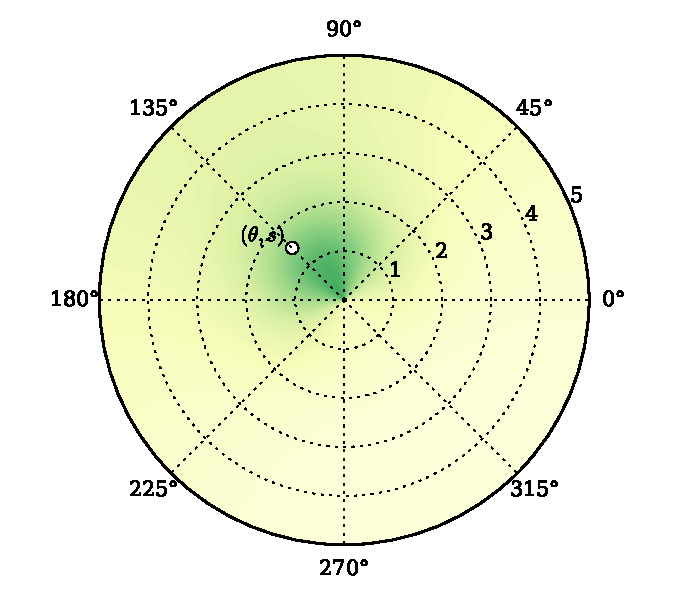
\includegraphics[width=.75\linewidth]{prob_shade}
	\vspace{-2em}
	\DIFdelbeginFL %DIFDELCMD < \captionof{figure}{Contour plot of the probability of occupying sampled at 121 points using $\theta_f=2\pi/3,v_w=1$}
%DIFDELCMD < 	%%%
\DIFdelendFL \DIFaddbeginFL \captionof{figure}{Colored plot of the probability of frond occupation sampled at 121 points using $\theta_f=2\pi/3,v_w=1$}
	\DIFaddendFL \label{fig:prob_shade}
\end{figure}
 \chapter{LIGHT MODEL}
\label{chap:light}

Now that we have formulated the distribution of kelp throughout the medium, we introduce the \DIFdelbegin \DIFdel{radiative transfer equation}\DIFdelend \DIFaddbegin \DIFadd{Radiative Transfer Equation}\DIFaddend , which is used to calculate the light field.

\section{Optical Definitions}

\subsection{Radiometric Quantities}

One of the most fundamental quantities in optics is radiant flux $\Phi$, which is the has units of energy per time.
The quantity of primary interest in modeling the light field is radiance $L$, which is defined as the radiant flux per steradian per projected surface area perpendicular to the direction of propagation of the beam.
That is,

\DIFdelbegin \begin{displaymath}
	\DIFdel{L = \frac{d^2\Phi}{dA d\omega}
}\end{displaymath}
%DIFAUXCMD
\DIFdelend \DIFaddbegin \begin{equation*}
	\DIFadd{L = \frac{d^2\Phi}{dA d\vec{\omega}}
}\end{equation*}
\DIFaddend 

Once the radiance $L$ is calculated everywhere, the irradiance is
\DIFdelbegin \begin{displaymath}
  \DIFdel{I(\vec{x}) = \int_{4\pi}L(\vec{x},\vec{\omega})\, d\omega.
}\end{displaymath}
%DIFAUXCMD
\DIFdelend \DIFaddbegin \begin{equation*}
  \DIFadd{I(\vec{x}) = \int_{4\pi}L(\vec{x},\vec{\omega})\, d\vec{\omega}.
}\end{equation*}
\DIFaddend Integrating $I(\vec{x})$, which has units \SI{}{\W/m^2}, over the surface of a frond, produces the power (with units \SI{}{\W}) transmitted to the frond.
\DIFdelbegin \DIFdel{This is discussed further in Section \ref{sec:perceived_irrad}}\DIFdelend \DIFaddbegin \DIFadd{For details, see Section \ref{sec:perceived_irrad}.
}\DIFaddend 

Irradiance \DIFdelbegin \DIFdel{can be converted to }\DIFdelend \DIFaddbegin \DIFadd{is sometimes given in units of }\DIFaddend moles of photons (\DIFdelbegin \DIFdel{also called Einsteins}\DIFdelend \DIFaddbegin \DIFadd{a mole of photons is also called an Einstein}\DIFaddend ) per second\DIFdelbegin \DIFdel{as
}\DIFdelend \DIFaddbegin \DIFadd{, with the conversion \mbox{%DIFAUXCMD
\cite{mobley_light_1994} }\hspace{0pt}%DIFAUXCMD
given by
}\DIFaddend \begin{equation}
  \SI{1}{\W\per\m^2} = \SI{4.2}{\micro\mole \,photons\per\second}.
  \DIFaddbegin \label{eqn:watts_photons}
\DIFaddend \end{equation}

\DIFaddbegin \subsection{\DIFadd{Perceived Irradiance}}
\label{sec:perceived_irrad}

\DIFadd{The average irradiance experienced by a kelp frond in depth layer $k$ is
}\newcommand{\Iperk}{\tilde{I}_k}
\begin{equation*}
   \DIFadd{\Iperk = \frac{\sum_{ij}P_{ijk}I_{ijk}}{\sum_{ij}P_{ijk}}.
}\end{equation*}

\DIFadd{The irradiance perceived by the kelp is expected to be slightly lower than the average irradiance,
}\begin{equation*}
  \DIFadd{\bar{I}_k = \frac{\sum_{ij}I_{ijk}}{n_x n_y}
}\end{equation*}
\DIFadd{since the kelp is more densely located at the center of the domain where the light field is reduced,
whereas the simple average is influenced by regions of higher irradiance at the edges of the domain where kelp is not present.
}

\DIFaddend \subsection{Inherent Optical Properties}
We must now define a few inherent optical properties (IOPs) which depend only on the medium of propagation.
These phenomena are governed by three inherent optical properties (IOPs) of the
medium.
The absorption coefficient $a(\vec{x})$ (units m$^{-1}$) defines the
proportional loss of radiance per unit length.
The scattering coefficient $b$ (units m$^{-1}$), defines the proportional loss
of radiance per unit length, and is assumed to be constant over space.

The volume scattering function (VSF) $\beta(\Delta): [-1, 1] \to \RR^+$ (units sr$^{-1}$) defines the probability of light scattering at any given angle from its source.
Formally, given two directions $\vec{\omega}$ and $\vec{\omega}'$, $\beta(\vec{\omega} \cdot \vec{\omega}')$ is the probability density of light scattering from $\vec{\omega}$ into $\vec{\omega}'$ (or vice-versa).
Of course, since a single direction subtends no solid angle, the probability of scattering occurring exactly from $\vec{\omega}$ to $\vec{\omega}'$ is 0.
Rather, we say that the probability of radiance being scattered from a direction $\omega$ into an element of solid angle $\Omega$ is $\int_\Omega \beta(\vec{\omega} \cdot \vec{\omega}')\, d\vec{\omega}'$.

The VSF is normalized such that
\DIFdelbegin \begin{displaymath}
  \DIFdel{\int_{-1}^1\beta(\Delta)\, d\Delta=\frac{1}{2\pi},
}\end{displaymath}
%DIFAUXCMD
\DIFdelend \DIFaddbegin \begin{equation*}
  \DIFadd{\int_{-1}^1\beta(\Delta)\, d\Delta=\frac{1}{2\pi},
}\end{equation*}
\DIFaddend so that for any $\omega$,
\DIFdelbegin \begin{displaymath}
  \DIFdel{\int_{4\pi}\beta(\vec{\omega}\cdot\vec{\omega}')\, d\vec{\omega}' = 1.
}\end{displaymath}
%DIFAUXCMD
\DIFdelend \DIFaddbegin \begin{equation*}
  \DIFadd{\int_{4\pi}\beta(\vec{\omega}\cdot\vec{\omega}')\, d\vec{\omega}' = 1.
}\end{equation*}
\DIFaddend i.e., the probability of light being scattered to some direction on the unit sphere is 1.


\section{The Radiative Transfer Equation}
\DIFaddbegin \DIFadd{We now present the Radiative Transfer Equation, whose solution is the radiance in the medium as a function of position and angle.
}\DIFaddend 

\subsection{Ray Notation}
Consider a fixed position $\vec{x}$ and direction $\vec{\omega}$ such that
$\vec{\omega} \cdot \hat{z} \neq 0$.
\DIFdelbegin %DIFDELCMD < 

%DIFDELCMD < %%%
\DIFdelend Let $\vec{l}(\vec{x}, \vec{\omega}, s)$ denote the linear path containing $\vec{x}$ \DIFaddbegin \DIFadd{in the direction $\vec{\omega}$.
Assume that the ray is not horizontal.
Then, it originates either at the surface or bottom of the domain, }\DIFaddend with initial z coordinate given by
\DIFdelbegin \begin{displaymath}
  \DIFdel{z_0 =
   \begin{cases}
    0, & \vec{\omega} \cdot \hat{z} < 0 \\
    \zmax, & \vec{\omega} \cdot \hat{z} > 0
  \end{cases}
}\end{displaymath}
%DIFAUXCMD
%DIFDELCMD < 

%DIFDELCMD < %%%
\DIFdel{Then, }\DIFdelend \DIFaddbegin \begin{equation*}
  \DIFadd{z_0 =
   \begin{cases}
    0, & \vec{\omega} \cdot \hat{z} < 0 \\
    \zmax, & \vec{\omega} \cdot \hat{z} > 0.
  \end{cases}
}\end{equation*}
\DIFadd{Hence, the ray path is parameterized as
}\DIFaddend \begin{equation}
  \vec{l}(\vec{x}, \vec{\omega}, s) = \frac{1}{\tilde{s}} (s\vec{x} + (\tilde{s} - s)\vec{x_0}(\vec{x}, \vec{\omega}))\DIFdelbegin %DIFDELCMD < \end{equation}
%DIFDELCMD < 

%DIFDELCMD < %%%
\DIFdel{where
}\begin{displaymath}
  \DIFdel{\vec{x_0}(\vec{x}, \vec{\omega}) = \vec{x} - \tilde{s} \vec{\omega}
}\end{displaymath}
%DIFAUXCMD
\DIFdelend \DIFaddbegin \DIFadd{,
  }\label{eqn:ray_path}
}
\DIFadd{where
}\begin{equation*}
  \DIFadd{\vec{x_0}(\vec{x}, \vec{\omega}) = \vec{x} - \tilde{s} \vec{\omega}
}\end{equation*}
\DIFaddend is the origin of the ray, and 
\DIFdelbegin %DIFDELCMD < 

%DIFDELCMD < %%%
\begin{displaymath}
  \DIFdel{\tilde{s} = \frac{\vec{x} \cdot \hat{z} - z_0}{\vec{\omega} \cdot \hat{z}}
}\end{displaymath}
%DIFAUXCMD
\DIFdelend \DIFaddbegin \begin{equation*}
  \DIFadd{\tilde{s} = \frac{\vec{x} \cdot \hat{z} - z_0}{\vec{\omega} \cdot \hat{z}}
}\end{equation*}
\DIFaddend is the path length from $\vec{x_0}(\vec{x}, \vec{\omega})$ to $\vec{x}$.

\subsection{Colloquial Description}
Denote the radiance at $\vec{x}$ in the direction $\vec{\omega}$ by $L(\vec{x}, \vec{\omega})$.
As light travels along $\vec{l}(\vec{x}, \vec{\omega}, s)$, interaction with the
medium produces three phenomena of interest:
\begin{enumerate}
  \item Radiance is decreased due to absorption.
  \item Radiance is decreased due to scattering out of the path to other
    directions.
  \item Radiance is increased due to scattering into the path from other
      directions.
\end{enumerate}

\subsection{Equation of Transfer}
\DIFdelbegin \DIFdel{Then, combining these phenomena , }\DIFdelend \DIFaddbegin \DIFadd{Combining these phenomena yields }\DIFaddend the Radiative Transfer \DIFdelbegin \DIFdel{equation }\DIFdelend \DIFaddbegin \DIFadd{Equation }\DIFaddend along
$\vec{l}(\vec{x}, \vec{\omega})$\DIFdelbegin \DIFdel{becomes
}\DIFdelend \DIFaddbegin \DIFadd{,
}\DIFaddend \begin{equation}
  \label{eqn:rte1d}
  \frac{dL}{ds}(\vec{l}(\vec{x}, \vec{\omega}, s), \vec{\omega})
  = -(a(\vec{x}) + b)L(\vec{x}, \vec{\omega})
  + b \int_{4\pi} \beta(\vec{\omega}\cdot\vec{\omega}') L(\vec{x})\, d\DIFdelbegin \DIFdel{\omega}\DIFdelend \DIFaddbegin \vec{\omega}\DIFaddend ',
\end{equation}
where $\int_{4\pi}$ denotes integration over the unit sphere.
\DIFdelbegin %DIFDELCMD < 

%DIFDELCMD < %%%
\DIFdel{Now, we have
}\begin{align*}
  \DIFdel{\frac{dL}{ds}(\vec{l}(\vec{x}, \vec{\omega}, s), \vec{\omega})
    }&\DIFdel{= \frac{d\vec{l}}{ds}(\vec{x}, \vec{\omega}, s) \cdot \nabla L(\vec{x}, \vec{\omega}', \vec{\omega}) }\\
    &\DIFdel{= \vec{\omega} \cdot \nabla L(\vec{x}, \vec{\omega})
}\end{align*}
%DIFAUXCMD
%DIFDELCMD < 

%DIFDELCMD < %%%
\DIFdel{Then, the }\DIFdelend \DIFaddbegin \DIFadd{The derivative of $L$ over the path can be rewritten as
}\begin{align*}
  \DIFadd{\frac{dL}{ds}(\vec{l}(\vec{x}, \vec{\omega}, s), \vec{\omega})
    }&\DIFadd{= \frac{d\vec{l}}{ds}(\vec{x}, \vec{\omega}, s) \cdot \nabla L(\vec{x}, \vec{\omega}', \vec{\omega}) }\\
    &\DIFadd{= \vec{\omega} \cdot \nabla L(\vec{x}, \vec{\omega}),
}\end{align*}
\DIFadd{which unveils the }\DIFaddend general form of the Radiative Transfer Equation\DIFdelbegin \DIFdel{is
}\begin{displaymath}
  \DIFdel{\vec{\omega} \cdot \nabla L(\vec{x}, \vec{\omega})
  = -(a(\vec{x}) + b)L(\vec{x}, \vec{\omega})
  + b \int_{4\pi} \beta(\vec{\omega}\cdot\vec{\omega}') L(\vec{x}, \vec{\omega}')\, d\omega'
}\end{displaymath}
%DIFAUXCMD
\DIFdelend \DIFaddbegin \DIFadd{,
}\begin{equation*}
  \DIFadd{\vec{\omega} \cdot \nabla L(\vec{x}, \vec{\omega})
  = -(a(\vec{x}) + b)L(\vec{x}, \vec{\omega})
  + b \int_{4\pi} \beta(\vec{\omega}\cdot\vec{\omega}') L(\vec{x}, \vec{\omega}')\, d\vec{\omega}'
}\end{equation*}
\DIFaddend 

or, equivalently,
\begin{equation}
  \vec{\omega} \cdot \nabla L(\vec{x}, \vec{\omega})
  + a(\vec{x})L(\vec{x}, \vec{\omega})
  = b \left(
    \int_{4\pi} \beta(\vec{\omega}\cdot\vec{\omega}') L(\vec{x}, \vec{\omega}')\, d\DIFdelbegin \DIFdel{\omega}\DIFdelend \DIFaddbegin \vec{\omega}\DIFaddend '
    - L(\vec{x}, \vec{\omega})
  \right)\DIFaddbegin \DIFadd{.
  }\label{eqn:rte}
\DIFaddend \end{equation}

\subsection{Boundary Conditions}

We use periodic boundary conditions in the $x$ and $y$ directions\DIFdelbegin \DIFdel{.
}\begin{align*}
  \DIFdel{L\left((\xmin, y, z), \vec{\omega}\right) }&\DIFdel{= L\left((\xmax, y, z), \vec{\omega}\right) }\\
  \DIFdel{L\left((x, \ymin, z), \vec{\omega}\right) }&\DIFdel{= L\left((x, \ymax, z), \vec{\omega}\right)
}\end{align*}
%DIFAUXCMD
%DIFDELCMD < 

%DIFDELCMD < %%%
\DIFdelend \DIFaddbegin \DIFadd{,
}\begin{align*}
  \DIFadd{L\left((\xmin, y, z), \vec{\omega}\right) }&\DIFadd{= L\left((\xmax, y, z), \vec{\omega}\right), }\\
  \DIFadd{L\left((x, \ymin, z), \vec{\omega}\right) }&\DIFadd{= L\left((x, \ymax, z), \vec{\omega}\right).
}\end{align*}
\DIFaddend In the $z$ direction, we specify a spatially uniform downwelling light just
under the surface of the water by a function $f(\vec{\omega})$.
Or if $\zmin>0$, then the radiance at $z=\zmin$ should be specified instead (as opposed to the radiance at the first grid cell center).
\DIFdelbegin %DIFDELCMD < 

%DIFDELCMD < %%%
\DIFdelend Further, we assume that no upwelling light enters the domain from the bottom\DIFdelbegin \DIFdel{.
}\begin{align*}
  \DIFdel{L(\vec{x_s}, \vec{\omega}) }&\DIFdel{= f(\omega) \mbox{ if } \vec{\omega} \cdot \hat{z} > 0}\\ 
  \DIFdel{L(\vec{x_b}, \vec{\omega}) }&\DIFdel{= 0 \mbox }{ \DIFdel{if }} \DIFdel{\vec{\omega} \cdot \hat{z} < 0
}\end{align*}
 %DIFAUXCMD
\DIFdelend \DIFaddbegin \DIFadd{, so
}\begin{align*}
  \DIFadd{L(\vec{x_s}, \vec{\omega}) }&\DIFadd{= f(\omega) \mbox{ if } \vec{\omega} \cdot \hat{z} > 0, }\\ 
  \DIFadd{L(\vec{x_b}, \vec{\omega}) }&\DIFadd{= 0 \mbox }{ \DIFadd{if }} \DIFadd{\vec{\omega} \cdot \hat{z} < 0.
}\end{align*}
 \DIFaddend 

\section{Low-Scattering Approximation}
In clear waters where absorption is more important than scattering, an asymptotic expansion can be used whereby the light field is generated through a sequence of discrete scattering events.
\subsection{Asymptotic Expansion}
Taking $b$ to be small, we introduce the asymptotic series
\newcommand{\Lasym}{L_0(\vec{x},\vec{\omega}) + b L_1(\vec{x},\vec{\omega}) + b^2 L_2(\vec{x},\vec{\omega}) + \cdots}
\newcommand{\Lasyms}{L_0(\vec{x_s},\vec{\omega}) + b L_1(\vec{x_s},\vec{\omega}) + b^2 L_2(\vec{x_s},\vec{\omega}) + \cdots}
\newcommand{\Lasymp}{L_0(\vec{x},\vec{\omega}') + b L_1(\vec{x},\vec{\omega}') + b^2 L_2(\vec{x},\vec{\omega}') + \cdots}
\DIFdelbegin \begin{align*}
  \DIFdel{L(\vec{x},\vec{\omega}) = \Lasym.
}\end{align*}
%DIFAUXCMD
\DIFdel{Then, substituting }\DIFdelend \DIFaddbegin \begin{align*}
  \DIFadd{L(\vec{x},\vec{\omega}) = \Lasym.
}\end{align*}
\DIFadd{Substituting }\DIFaddend the above into \DIFdelbegin \DIFdel{the RTE,
}\begin{displaymath}
  \DIFdel{\begin{split}
    &\vec{\omega} \cdot \nabla \left[ \Lasym \right] \\
    &+ a(\vec{x}) \left[ \Lasym \right] \\
    &= b\Bigg(
      \int_{4\pi} \beta(\abs{\vec{\omega} - \vec{\omega}'})
      \left[ \Lasymp \right] \, d\vec{\omega}' \\
    &- \left[ \Lasym \right]
    \Bigg)
    \end{split}
}\end{displaymath}
%DIFAUXCMD
\DIFdel{Then, grouping }\DIFdelend \DIFaddbegin \eqref{eqn:rte} \DIFadd{yields
}\begin{align*}
    &\DIFadd{\vec{\omega} \cdot \nabla \left[ \Lasym \right] }\\
    &\DIFadd{+ a(\vec{x}) \left[ \Lasym \right] }\\
    &\DIFadd{= b\Bigg(
      \int_{4\pi} \beta(\vec{\omega}\cdot\vec{\omega}')
      \left[ \Lasymp \right] \, d\vec{\omega}' }\\
    &\DIFadd{- \left[ \Lasym \right]
    \Bigg).
}\end{align*}
\DIFadd{Grouping }\DIFaddend like powers of $b$, we have the decoupled set of equations
\begin{align}
  \vec{\omega} \cdot \nabla L_0(\vec{x}, \vec{\omega}) + a(\vec{x})L_0(\vec{x}) &= 0\DIFaddbegin \DIFadd{,
  }\label{eqn:asymptotics_0}\DIFaddend \\
  \vec{\omega} \cdot \nabla L_1(\vec{x}, \vec{\omega}) + a(\vec{x})L_1(\vec{x})
  &= \int_{4\pi} \beta(\DIFdelbegin %DIFDELCMD < \abs{\vec{\omega} - \vec{\omega}'}%%%
\DIFdelend \DIFaddbegin \vec{\omega}\DIFadd{\cdot}\vec{\omega}\DIFadd{'}\DIFaddend ) L_0(\vec{x}, \vec{\omega}')\,d\vec{\omega}' - L_0(\vec{x}, \vec{\omega})\DIFaddbegin \DIFadd{, }\nonumber\DIFaddend \\ 
  \vec{\omega} \cdot \nabla L_2(\vec{x}, \vec{\omega}) + a(\vec{x})L_2(\vec{x})
  &= \int_{4\pi} \beta(\DIFdelbegin %DIFDELCMD < \abs{\vec{\omega} - \vec{\omega}'}%%%
\DIFdelend \DIFaddbegin \vec{\omega}\DIFadd{\cdot}\vec{\omega}\DIFadd{'}\DIFaddend ) L_1(\vec{x}, \vec{\omega}')\,d\vec{\omega}' - L_1(\vec{x}, \vec{\omega})\DIFaddbegin \DIFadd{. }\nonumber \DIFaddend \\ 
  &\vdots \nonumber
\end{align}
\DIFaddbegin \DIFadd{In general, for $n \geq 1$,
}\begin{equation}
  \DIFadd{\vec{\omega} \cdot \nabla L_n(\vec{x}, \vec{\omega}) + a(\vec{x})L_n(\vec{x})
  = \int_{4\pi} \beta(\vec{\omega}\cdot\vec{\omega}') L_{n-1}(\vec{x}, \vec{\omega}')\,d\vec{\omega}' - L_{n-1}(\vec{x}, \vec{\omega}).
  \label{eqn:asymptotics_n}
}\end{equation}
\DIFaddend 

For boundary conditions, let \DIFdelbegin \DIFdel{$x_s$ }\DIFdelend \DIFaddbegin \DIFadd{$\vec{x_s}$ }\DIFaddend be a point on the surface of the domain.
Then, 
\DIFdelbegin \begin{displaymath}
  \DIFdel{\Lasyms =
  \begin{cases}
    f(\omega), & \hat{z}\cdot\omega > 0 \\
    0, & \mbox{otherwise},
  \end{cases}
}\end{displaymath}
%DIFAUXCMD
\DIFdel{which becomes
}\DIFdelend \DIFaddbegin \begin{equation*}
  \DIFadd{\Lasyms =
  \begin{cases}
    f(\omega), & \hat{z}\cdot\omega > 0 \\
    0, & \mbox{otherwise},
  \end{cases}
}\end{equation*}
\DIFadd{which can be decomposed as
}\DIFaddend \begin{align}
  L_0(\vec{x}, \vec{\omega}) &=
  \begin{cases}
    f(\omega), & \hat{z}\cdot\omega > 0, \\
    0, & \mbox{otherwise},
  \end{cases}
  \DIFaddbegin \label{eqn:asymptotics_bc_0} \DIFaddend \\
  L_1(\vec{x}, \vec{\omega}) &= 0 \DIFaddbegin \nonumber \DIFaddend \\
  L_2(\vec{x}, \vec{\omega}) &= 0. \DIFaddbegin \nonumber \DIFaddend \\
  &\vdots \nonumber
\end{align}
\DIFaddbegin \DIFadd{In general, for $n \geq 1$,
}\begin{equation}
  \DIFadd{L_n(\vec{x}, \vec{\omega}) = 0.
  \label{eqn:asymptotics_bc_n}
}\end{equation}
\DIFaddend 

 
\subsection{Analytical Solution}
\label{sec:asymptotic_sol}

For all $\vec{x}, \vec{\omega}$, \DIFdelbegin \DIFdel{let
}\begin{align*}
  \DIFdel{\tilde{a}(s) }&\DIFdel{= a(\vec{l}(\vec{x}, \vec{\omega}), s), }\\ 
  \DIFdel{\frac{du_0}{ds}(s) + \tilde{a}(s) u_0(s) }&\DIFdel{= 0, u_0(0) = f(\vec{\omega})
}\end{align*}
%DIFAUXCMD
\DIFdel{Then, }\begin{align*}
  \DIFdel{u_0(s) = f(\omega) \exp\left(-\int_0^s \tilde{a}(s)\, ds\right), }\\
  \DIFdel{L_0(\vec{l}(\vec{x}, \vec{\omega},s), \vec{\omega}) = u_0(s)
}\end{align*}
%DIFAUXCMD
\DIFdelend \DIFaddbegin \DIFadd{we consider the path $l(\vec{x}, \vec{\omega}, s)$ from }\eqref{eqn:ray_path}\DIFadd{.
We extract the absorption coefficient along the path,
}\begin{equation*}
  \DIFadd{\tilde{a}(s) = a(\vec{l}(\vec{x}, \vec{\omega}), s).
}\end{equation*}
\DIFadd{Then, the first equation from the asymptotic expansion, }\eqref{eqn:asymptotics_0} \DIFadd{and its associated boundary condition, }\eqref{eqn:asymptotics_bc_0}\DIFadd{, can be rewritten as
}\begin{equation*}
  \DIFadd{\left\{
  \begin{aligned}
  0 &= \frac{du_0}{ds}(s) + \tilde{a}(s) u_0(s) \\
  u_0(0) &= f(\vec{\omega}),
  \end{aligned}
  \right.
}\end{equation*}
\DIFadd{which we can solve by multiplying by the appropriate integrating factor, as follows.
}\begin{align*}
  \DIFadd{0 }&\DIFadd{= \exp\left(\int_0^s \tilde{a}(s')\, ds'\right) \frac{du_0}{ds} + \exp\left(\int_0^s \tilde{a}(s')\, ds'\right) \tilde{a}(s) u_0(s) }\\
  &\DIFadd{= \frac{d}{ds}\left[\exp\left(\int_0^s \tilde{a}(s')\, ds'\right) u_0(s)\right].
}\end{align*}
\DIFadd{Then, integrating both sides yields
}\begin{align*}
  \DIFadd{0 }&\DIFadd{= \int_0^s \frac{d}{ds'}\left[\exp\left(\int_0^{s'} \tilde{a}(s'')\, ds''\right) u_0(s')\right]\, ds' }\\
  &\DIFadd{= \exp\left(\int_0^s \tilde{a}(s')\, ds'\right) u_0(s) - f(\vec{\omega}).
}\end{align*}
\DIFadd{Hence,
}\begin{equation}
  \DIFadd{u_0(s) = f(\omega) \exp\left(-\int_0^s \tilde{a}(s)\, ds\right).
  \label{eqn:asymptotics_soln_0}
}\end{equation}
\DIFadd{Then, we convert back from path length $s$ to the spatial coordinate $\vec{x}$ using
}\begin{equation*}
  \DIFadd{L_0(\vec{l}(\vec{x}, \vec{\omega},s), \vec{\omega}) = u_0(s).
}\end{equation*}
\DIFaddend 

\DIFdelbegin \begin{align*}
  \DIFdel{g_n(s) = \int_{4\pi} \beta(\abs{\vec{\omega} - \vec{\omega}'})
  L_{n-1}(\vec{l}(\vec{x}, \vec{\omega'}, s), \vec{\omega}')\,d\vec{\omega}' - L_{n-1}(\vec{l}(\vec{x}, \vec{\omega}, s), \vec{\omega}) }\\ 
  \DIFdel{\frac{du_n}{ds}(s) + \tilde{a}(s)u_n(s) = g_n(s), u_n(0) = 0
}\end{align*}
%DIFAUXCMD
%DIFDELCMD < 

%DIFDELCMD < %%%
\DIFdel{Then, }\begin{align*}
  \DIFdel{u_n(s) = \int_0^sg_n(s')\exp\left( -\int_{s''}^{s'}\tilde{a}(s'')\,ds'' \right)\, ds' }\\
  \DIFdel{L_n(\vec{l}(\vec{x}, \vec{\omega}, s), \vec{\omega}) = u_n(s)
}\end{align*}
 %DIFAUXCMD
\DIFdelend \DIFaddbegin \DIFadd{The $n \geq 1$ equations have a nonzero right-hand side, which we call the effective source, $g_n(s)$.
This can be similarly extracted along a ray path as
}\begin{equation*}
  \DIFadd{g_n(s) = \int_{4\pi} \beta(\vec{\omega}\cdot\vec{\omega}')
  L_{n-1}(\vec{l}(\vec{x}, \vec{\omega'}, s), \vec{\omega}')\,d\vec{\omega}' - L_{n-1}(\vec{l}(\vec{x}, \vec{\omega}, s), \vec{\omega}).
}\end{equation*}
\DIFadd{Then, since $g_n$ depends only on $L_{n-1}$, it is independent of $u_n$, which allows }\eqref{eqn:asymptotics_n} \DIFadd{and its boundary condition, }\eqref{eqn:asymptotics_bc_n}\DIFadd{, to be written as the first order, linear ordinary differential equation along the ray path,
}\begin{equation*}
  \DIFadd{\left\{
  \begin{aligned}
    g_n(s) &= \frac{du_n}{ds}(s) + \tilde{a}(s)u_n(s) \\
    u_n(0) &= 0
  \end{aligned}
  \right.
}\end{equation*}
\DIFadd{As with the $n=0$ equation, the solution is found by multiplying by the appropriate integrating factor.
}\begin{align*}
  \DIFadd{\exp\left(\int_0^s \tilde{a}(s')\, ds'\right) g_n(s) }&\DIFadd{= \exp\left(\int_0^s \tilde{a}(s')\, ds'\right) \frac{du_n}{ds} + \exp\left(\int_0^s \tilde{a}(s')\, ds'\right) \tilde{a}(s) u_n(s) }\\
  &\DIFadd{= \frac{d}{ds}\left[\exp\left(\int_0^s \tilde{a}(s')\, ds'\right) u_n(s)\right].
}\end{align*}
\DIFadd{Integrating both sides yields
}\begin{align*}
  \DIFadd{\int_0^s\exp\left(\int_0^{s'} \tilde{a}(s'')\, ds''\right) g_n(s')\, ds' }&\DIFadd{= \int_0^s \frac{d}{ds'}\left[\exp\left(\int_0^{s'} \tilde{a}(s'')\, ds''\right) u_n(s')\right]\, ds' }\\
  &\DIFadd{= \exp\left(\int_0^s \tilde{a}(s')\, ds'\right) u_n(s).
}\end{align*}
\DIFadd{Hence,
}\begin{equation*}
  \DIFadd{u_n(s) = \exp\left(-\int_0^s \tilde{a}(s')\, ds'\right) \int_0^s\exp\left(\int_0^{s'} \tilde{a}(s'')\, ds''\right) g_n(s')\, ds',
}\end{equation*}
\DIFadd{which simplifies to
}\begin{equation}
  \DIFadd{u_n(s) = \int_0^sg_n(s')\exp\left( -\int_{s''}^{s'}\tilde{a}(s'')\,ds'' \right)\, ds'.
  \label{eqn:asymptotics_soln_n}
}\end{equation}
\DIFadd{As before, the conversion back to spatial coordinates is
}\begin{equation*}
  \DIFadd{L_n(\vec{l}(\vec{x}, \vec{\omega}, s), \vec{\omega}) = u_n(s).
}\end{equation*}
 \DIFaddend \chapter{NUMERICAL SOLUTION}
\label{chap:numerical}

In this chapter, the mathematical details involved in the numerical solution of the previously described equations are presented.
It is assumed that this model is run in conjunction with a model describing the growth of kelp over its life cycle, which calls this light model periodically to update the light field.

\section{Super-Individuals}
\DIFaddbegin \label{sec:si}
\DIFaddend 

\DIFdelbegin \DIFdel{The algorithm described in this chapter has two components.
First, a probabilistic description of the kelp is generated at each point in a discrete spatial grid.
Second, optical properties of the resulting kelp-water medium are derived, and the light field is calculated.
The first component is described here.
}%DIFDELCMD < 

%DIFDELCMD < %%%
\subsection{\DIFdel{Frond Length Distribution}}
%DIFAUXCMD
\addtocounter{subsection}{-1}%DIFAUXCMD
%DIFDELCMD < 

%DIFDELCMD < %%%
\DIFdelend Rather than model each kelp frond, a subset of the population, called super-individuals, are \DIFdelbegin \DIFdel{modelled }\DIFdelend \DIFaddbegin \DIFadd{modeled }\DIFaddend explicitly, and are considered to represent many identical individuals, as in \citep{scheffer_super-individuals_1994}.
Specifically, at each depth $k$, there are $n$ super-individuals, indexed by $i$.
Super-individual $i$ has a frond area $A_{ki}$ and represents $n_{ki}$ individual fronds.

From \eqref{eqn:length-from-area}, the frond length of the super-individual is $l_{ki} = \sqrt{2A_{ki}f_r}$.
Given the super-individual data, we calculate the mean $\mu$ and standard deviation $\sigma$ frond
lengths using the formulas
\DIFdelbegin \DIFdel{:
}\begin{displaymath}
  \DIFdel{\mu_k = \frac{\ds \sum_{i=1}^N l_{ki}}{\ds \sum_{i=1}^N n_{ki}},
}\end{displaymath}
%DIFAUXCMD
\begin{displaymath}
  \DIFdel{\sigma_k = \frac{\ds \sum_{i=1}^N \left( l_{ki} - \mu_k \right)^2}{\ds \sum_{i=1}^N n_{ki}}.
}\end{displaymath}
%DIFAUXCMD
\DIFdelend \DIFaddbegin \begin{align}
  \DIFadd{\mu_k }&\DIFadd{= \frac{\ds \sum_{i=1}^N l_{ki}}{\ds \sum_{i=1}^N n_{ki}},
  \label{eqn:si_mean} }\\
  \DIFadd{\sigma_k }&\DIFadd{= \frac{\ds \sum_{i=1}^N \left( l_{ki} - \mu_k \right)^2}{\ds \sum_{i=1}^N n_{ki}}.
  \label{eqn:si_std}
}\end{align}
\DIFaddend We then assume that frond lengths are normally distributed in each depth layer
with mean $\mu_k$ and standard deviation $\sigma_k$.

\section{Discrete Grid}
\DIFaddbegin \label{sec:grid}

\DIFaddend The following is a description of the \DIFdelbegin \DIFdel{uniform, rectangular }\DIFdelend spatial-angular grid used in the numerical implementation of this model.
It is assumed that all simulated quantities are constant over the interior of a grid cell.
\DIFaddbegin \DIFadd{Other legitimate choices of grids exists; this one was chosen for its relative simplicity.
}\DIFaddend 

The \DIFaddbegin \DIFadd{domain of the radiative transfer equation is embedded in five dimensions: three spatial ($x$, $y$, and $z$) and two angular (azimuthal $\theta$ and polar $\phi$).
The }\DIFaddend number of grid cells in each dimension are denoted by $n_x$, $n_y$, $n_z$,
$n_\theta$, and $n_\phi$, with uniform spacings $dx$, $dy$, $dz$, $d\theta$, and
$d\phi$ between adjacent grid points.

The following indices are assigned to each dimension:
\DIFdelbegin \begin{align*}
  \DIFdel{x }&\DIFdel{\to i }\\
  \DIFdel{y }&\DIFdel{\to j }\\
  \DIFdel{z }&\DIFdel{\to k }\\
  \DIFdel{\theta }&\DIFdel{\to l }\\
  \DIFdel{\phi }&\DIFdel{\to m
}\end{align*}
%DIFAUXCMD
\DIFdelend \DIFaddbegin \begin{align*}
  \DIFadd{x }&\DIFadd{\to i }\\
  \DIFadd{y }&\DIFadd{\to j }\\
  \DIFadd{z }&\DIFadd{\to k }\\
  \DIFadd{\theta }&\DIFadd{\to l }\\
  \DIFadd{\phi }&\DIFadd{\to m
}\end{align*}
\DIFaddend 

It is convenient, however, to use a single index $p$ to refer to directions $\vec{\omega}$ rather than referring to $\theta$ and $\phi$ separately.
Then, the center of a generic grid cell will be denoted as
$(x_i, y_j, z_k, \vec{\omega}_p)$, and the boundaries between adjacent grid cells
will be referred to as \textit{edges}.
One-indexing is employed throughout this document.

\DIFdelbegin \subsection{\DIFdel{Spatial Grid}}
%DIFAUXCMD
\addtocounter{subsection}{-1}%DIFAUXCMD
\DIFdelend \begin{figure}[H]
  \centering
  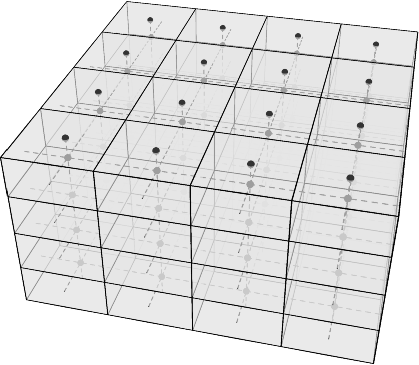
\includegraphics[width=8cm]{spatialgrid.pdf}
  \caption{Spatial grid}
  \label{fig:spatial_grid}
\end{figure}

\DIFdelbegin \begin{align*}
  \DIFdel{dx }&\DIFdel{= \frac{x_{\max}-x_{\min}}{n_x} }\\ 
  \DIFdel{dy }&\DIFdel{= \frac{y_{\max}-y_{\min}}{n_y} }\\ 
  \DIFdel{dz }&\DIFdel{= \frac{z_{\max}-z_{\min}}{n_z}
}\end{align*}
%DIFAUXCMD
%DIFDELCMD < 

%DIFDELCMD < %%%
\DIFdel{Denote the edges as 
}\begin{align*}
  \DIFdel{x_i^e }&\DIFdel{= (i-1)x \mbox{ for } i=1,\ldots,n_x }\\
  \DIFdel{y_j^e }&\DIFdel{= (j-1)y \mbox{ for } j=1,\ldots,n_y }\\
  \DIFdel{z_k^e }&\DIFdel{= (k-1)z \mbox{ for } k=1,\ldots,n_z 
}\end{align*}
%DIFAUXCMD
%DIFDELCMD < 

%DIFDELCMD < %%%
\DIFdel{and the cell centers as
}\begin{align*}
  \DIFdel{x_i }&\DIFdel{= (i-1/2)dx \mbox{ for } i=1,\ldots,n_x }\\
  \DIFdel{y_j }&\DIFdel{= (j-1/2)dy \mbox{ for } j=1,\ldots,n_y }\\
  \DIFdel{z_k }&\DIFdel{= (k-1/2)dz \mbox{ for } k=1,\ldots,n_z
}\end{align*}
%DIFAUXCMD
%DIFDELCMD < 

%DIFDELCMD < %%%
\DIFdel{Note that in this convention, there are the same number of edges and cells, and edges preceed centers.
}%DIFDELCMD < 

%DIFDELCMD < %%%
\DIFdelend \DIFaddbegin \DIFadd{Each spatial grid cell is the Cartesian product of $x$, $y$, and $z$ intervals of width $dx$, $dy$, and $dz$ respectively.
The three-dimensional interval centered at $(x_i, y_j, z_k)$ is denoted $X_{ijk}$, and has volume $\abs{X_{ijk}}=dx\,dy\,dz$.
}\DIFaddend Also, note that no grid center is located on the plane $z=0$\DIFdelbegin \DIFdel{.
The }\DIFdelend \DIFaddbegin \DIFadd{; the }\DIFaddend surface radiance boundary condition is treated separately.

\DIFdelbegin \subsection{\DIFdel{Angular Grid}}
%DIFAUXCMD
\addtocounter{subsection}{-1}%DIFAUXCMD
\DIFdelend \begin{figure}[H]
  \centering
  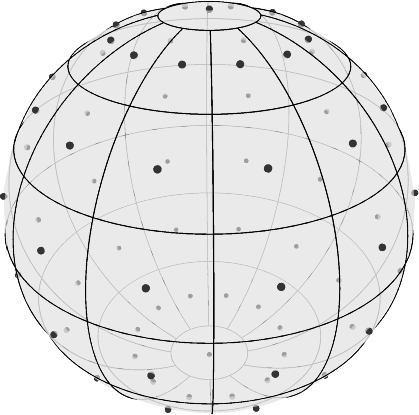
\includegraphics[width=8cm]{angulargrid.pdf}
  \caption{Angular grid at each point in space}
  \label{fig:angular_grid}
\end{figure}

\DIFdelbegin \DIFdel{Now, we define the azimuthal angle such that
}\begin{align*}
  \DIFdel{\theta_l = (l-1)d\theta.
}\end{align*}
%DIFAUXCMD
\DIFdel{For the sake of periodicity, we need
}\begin{align*}
  \DIFdel{\theta_1 }&\DIFdel{= 0, }\\
  \DIFdel{\theta_{n_\theta} }&\DIFdel{= 2\pi-d\theta,
}\end{align*}
%DIFAUXCMD
\DIFdel{which requires
}\begin{displaymath}
  \DIFdel{d\theta = \frac{2\pi}{n_\theta}.
}\end{displaymath}
%DIFAUXCMD
%DIFDELCMD < 

%DIFDELCMD < %%%
\DIFdel{For the polar angle, we similarly let
}\begin{displaymath}
  \DIFdel{\phi_m = (m-1)d\phi
}\end{displaymath}
%DIFAUXCMD
%DIFDELCMD < 

%DIFDELCMD < %%%
\DIFdel{Since the polar azimuthal is not periodic, we also store the endpoint, so
}\begin{align*}
  \DIFdel{\phi_1 }&\DIFdel{= 0, }\\
  \DIFdel{\phi_{n_\phi} }&\DIFdel{= \pi.
}\end{align*}
%DIFAUXCMD
%DIFDELCMD < 

%DIFDELCMD < %%%
\DIFdel{This gives us
}\begin{align*}
  \DIFdel{d\phi }&\DIFdel{= \frac{\pi}{n_\phi-1}.
}\end{align*}
%DIFAUXCMD
%DIFDELCMD < 

%DIFDELCMD < %%%
\DIFdel{It is also useful to define the edges between angular grid cells as
}\begin{align*}{\DIFdel{3}}
  \DIFdel{\theta_l^e }&\DIFdel{= (l-1/2) d\theta, }&\DIFdel{\quad l}&\DIFdel{=1,\ldots,n_\theta }\\
  \DIFdel{\phi_m^e }&\DIFdel{= (m-1/2) d\phi, }&\DIFdel{\quad m}&\DIFdel{=1,\ldots,n_\phi-1.
}\end{align*}
%DIFAUXCMD
%DIFDELCMD < 

%DIFDELCMD < %%%
\DIFdel{Note that while $\theta$ has its final edge following its final center, this is
not the case for $\phi$.
}%DIFDELCMD < 

%DIFDELCMD < \begin{figure}[h]
%DIFDELCMD <   \centering
%DIFDELCMD <   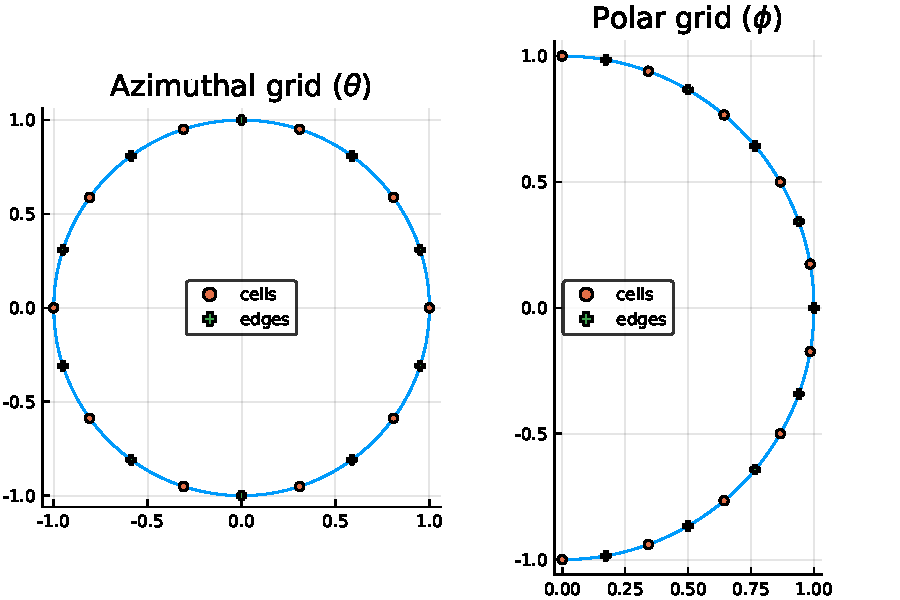
\includegraphics[width=.75\linewidth]{angular_grid_plots}
%DIFDELCMD <   %%%
%DIFDELCMD < \caption{%
{%DIFAUXCMD
\DIFdelFL{Angular grid}}
%DIFAUXCMD
%DIFDELCMD < \end{figure}
%DIFDELCMD < 

%DIFDELCMD < %%%
\DIFdelend As shown in Figure \ref{fig:angular_grid}, $\phi=0$ and $\phi=\pi$, called
the north ($+z$) and south ($-z$) poles respectively, are treated separately \DIFdelbegin \DIFdel{.
The total number of angles considered is $n_{\vec{\omega}} = n_\phi n_\theta -
2(n_\theta-1)$.
Since the poles create a non-rectangular angular grid in the sense that
$n_{\vec{\omega}}$ is not the product of two integers, it is advantageous to use
a single variable $p=1,\ldots,n_{\vec{\omega}}$ to index angles $\vec{\omega} =
(\theta, \phi)$ such that $p \in \left\{ 2,\ldots,n_{\vec{\omega}}-1 \right\}$ refers to the interior
of }\DIFdelend \DIFaddbegin \DIFadd{from other angular grid cells.
A generic interior angular grid cell centered at $\vec{\omega}_p$ is }\DIFaddend the \DIFdelbegin \DIFdel{angular grid, and }\DIFdelend \DIFaddbegin \DIFadd{Cartesian product of an azimuthal interval of width $d\theta$ and a polar interval of width $d\theta$.
However, two pole cells are the Cartesian product of a polar interval of width $d\phi/2$ and the full azimuthal domain, $[0, 2\pi)$.
}

\DIFadd{With this configuration, the total number of angles considered is $\nomega = n_\theta(n_\phi-2)+2$.
Then, cells are indexed by $p=1,\ldots,n_{\vec{\omega}}$ and are ordered such that
}\DIFaddend $p=1$ and $p=n_{\vec{\omega}}$ refer to the north and south poles respectively\DIFdelbegin \DIFdel{.
The following notation is used.
}\begin{align*}
  \DIFdel{\hat{l}(p) }&\DIFdel{= \mbox{mod1}(p, n_\theta) }\\
  \DIFdel{\hat{m}(p) }&\DIFdel{= \ceil(p/n_\theta) + 1 }\\
  \DIFdel{\hat{\theta}_p }&\DIFdel{= \theta_{\hat{l}(p)} }\\
  \DIFdel{\hat{\phi}_p }&\DIFdel{= \phi_{\hat{m}(p)}
}\end{align*}
%DIFAUXCMD
%DIFDELCMD < 

%DIFDELCMD < %%%
\DIFdel{Thus,
it follows that
}\begin{displaymath}
  \DIFdel{p = \left( \hat{m}(p)-2\right)n_\theta + \hat{l}(p).
}\end{displaymath}
%DIFAUXCMD
%DIFDELCMD < 

%DIFDELCMD < %%%
\DIFdel{Accordingly, define
}\begin{displaymath}
  \DIFdel{\hat{p}(l,m) = (m-1)n_\theta + l.
}\end{displaymath}
%DIFAUXCMD
%DIFDELCMD < 

%DIFDELCMD < %%%
\DIFdel{Further, we }\DIFdelend \DIFaddbegin \DIFadd{,
$p\leq\nomega/2$ refers to the northern hemisphere, and $p>\nomega/2$ refers to the southern hemisphere.
Further, the symbol $\Omega_p$ is used to }\DIFaddend refer to the \DIFdelbegin \DIFdel{angular grid cell centered at $\vec{\omega}_p$ as $\Omega_p$, and the }\DIFdelend \DIFaddbegin \DIFadd{two dimension angular interval centered at $\omega_p$.
The }\DIFaddend solid angle subtended by $\Omega_p$ is denoted $\abs{\Omega_p}$.
\DIFdelbegin \DIFdel{The areas of the grid cells are calculated as follows.
Note that there is a temporary abuse of notation in that the same symbols ($d\theta$ and $d\phi$) are being used for infinitessimal differential and for finite gridspacing}\DIFdelend \DIFaddbegin \DIFadd{Refer to Appendix \ref{chap:grid_details} for a more rigorous discussion of the discrete spatial-angular grid}\DIFaddend .

\DIFdelbegin \DIFdel{For the poles, we have
}\begin{align*}
  \DIFdel{\abs{\Omega_1} = \abs{\Omega_\nomega} }&\DIFdel{= \int_{\Omega_1} d}{\DIFdel{\vec{\omega}}} \\
  &\DIFdel{= \int_0^{2\pi}\int_0^{d\phi/2} \sin\phi\, d\phi\, d\theta }\\
  &\DIFdel{= 2\pi \cos\phi \Big|_{d\phi/2}^0 }\\
  &\DIFdel{= 2\pi(1-\cos(d\phi/2))
}\end{align*}
%DIFAUXCMD
%DIFDELCMD < 

%DIFDELCMD < %%%
\DIFdel{And for all other angular grid cells,
}\begin{align*}
  \DIFdel{\abs{\Omega_p} }&\DIFdel{= \int_{\Omega_p} d}{\DIFdel{\vec{\omega}}} \\
                 &\DIFdel{= \int_{\theta_l^e}^{\theta_{l+1}^e}\int_{\phi_m^e}^{\phi_{m+1}^e} \sin(\phi)\, d\phi\, d\theta }\\
                 &\DIFdel{= d\theta \int_{\phi_m^e}^{\phi_{m+1}^e} \sin(\phi)\, d\phi }\\
                 &\DIFdel{= d\theta\left( \cos(\phi_m^e)-\cos(\phi_{m+1}^e) \right).
}\end{align*}
%DIFAUXCMD
%DIFDELCMD < 

%DIFDELCMD < %%%
\subsection{\DIFdel{Angular Quadrature}}
%DIFAUXCMD
\addtocounter{subsection}{-1}%DIFAUXCMD
\DIFdel{We assume }\DIFdelend \DIFaddbegin \section{\DIFadd{Quadrature Rules}}
\DIFadd{Since it is assumed }\DIFaddend that all quantities are constant within a spatial-angular grid cell\DIFdelbegin \DIFdel{.
We therefore employ }\DIFdelend \DIFaddbegin \DIFadd{,
}\DIFaddend the midpoint rule \DIFaddbegin \DIFadd{is employed }\DIFaddend for both spatial and angular integration.
\DIFaddbegin \DIFadd{Presented here is a basic derivation of the formulas for integration in the spatial-angular grid.
Further details are found in Appendix \ref{chap:ray_tracing}.
}\DIFaddend 

\DIFdelbegin \DIFdel{Define the }\DIFdelend \DIFaddbegin \subsection{\DIFadd{Spatial Quadrature}}
\DIFadd{Define the }\textit{\DIFadd{spatial characteristic function}} \DIFadd{as
}\begin{equation*}
  \DIFadd{\mathcal{X}^X_{ijk}(\vec{x}) = \begin{cases}
    1, & \vec{x} \in X_{ijk} \\
    0, & \mbox{otherwise}.
  \end{cases}
}\end{equation*}
\DIFadd{The double integral of a function $f(\vec{x})$ over a depth layer $k$ is approximated as
}\begin{align*}
  \DIFadd{\int_\xmin^\xmax\int_\ymin^\ymax f(x, y, z_k)\, dy\, dx }&\DIFadd{\approx \int_\xmin^\xmax \int_\ymin^\ymax \sum_{i=1}^{n_x}\sum_{j=1}^{n_y} \mathcal{X}^X_{ijk}(x,y,z_k) f(x_i, y_j, z_k)\, dy\, dx }\\
  &\DIFadd{= \sum_{i=1}^{n_x}\sum_{j=1}^{n_y} f(x_i, y_j, z_k) \int_\xmin^\xmax \int_\ymin^\ymax \mathcal{X}^X_{ijk}(x,y,z_k) \, dy\, dx }\\
  &\DIFadd{= \sum_{i=1}^{n_x}\sum_{j=1}^{n_y} \abs{X_{ijk}} f(x_i, y_j, z_k) }\\
  &\DIFadd{= dx\, dy\, dx\, \sum_{i=1}^{n_x}\sum_{j=1}^{n_y} f(x_i, y_j, z_k).
}\end{align*}
\DIFadd{The path integral of $f(\vec{x})$ over a path $\vec{l}(s)$ from $s=0$ to $s=\tilde{s}$ is
}\begin{align*}
  \DIFadd{\int_0^{\tilde{s}} f(\vec{l}(s))\, ds }&\DIFadd{= \sum_{i=1}^{n_x}\sum_{j=1}^{n_y}\sum_{k=1}^{n_z} f(x_i, y_j, z_k)\, ds_{ijk},
}\end{align*}
\DIFadd{where $ds_{ijk}$ is the total path distance of $\vec{l}(s)$ through $X_{ijk}$.
Full details of the path integral algorithm for the case of straight line paths are found in Appendix \ref{chap:ray_tracing}.
}

\subsection{\DIFadd{Angular Quadrature}}
\DIFadd{Define the }\DIFaddend \textit{angular characteristic function} \DIFdelbegin \begin{displaymath}
  \DIFdel{\mathcal{X}^\Omega_p(\vec{\omega}) = \begin{cases}
    1, & \vec{\omega} \in \Omega_p \\
    0, & \mbox{otherwise}
  \end{cases}
}\end{displaymath}
%DIFAUXCMD
\DIFdelend \DIFaddbegin \DIFadd{as
}\begin{equation*}
  \DIFadd{\mathcal{X}^\Omega_p(\vec{\omega}) = \begin{cases}
    1, & \vec{\omega} \in \Omega_p \\
    0, & \mbox{otherwise}.
  \end{cases}
}\end{equation*}
\DIFaddend 


\DIFdelbegin \begin{align*}
  \DIFdel{\int_{4\pi} f(\vec{\omega})\, d\vec{\omega} }&\DIFdel{= \int_{4\pi} \sum_{p=1}^\nomega f_p \mathcal{X}^\Omega_p(\vec{\omega})\, d\vec{\omega} }\\
  &\DIFdel{= \sum_{p=1}^\nomega f_p \int_{4\pi} \mathcal{X}^\Omega_p(\vec{\omega})\, d\vec{\omega} }\\
  &\DIFdel{= \sum_{p=1}^\nomega f_p \int_{\Omega_p} d\vec{\omega} }\\
  &\DIFdel{= \sum_{p=1}^\nomega f_p \abs{\Omega_p}
}\end{align*}
%DIFAUXCMD
\DIFdelend \DIFaddbegin \DIFadd{Then, the integral of a function $f(\vec{\omega})$ is approximated as
}\begin{align*}
  \DIFadd{\int_{4\pi} f(\vec{\omega})\, d\vec{\omega} }&\DIFadd{\approx \int_{4\pi} \sum_{p=1}^\nomega f(\vec{\omega}_p) \mathcal{X}^\Omega_p(\vec{\omega})\, d\vec{\omega} }\\
  &\DIFadd{= \sum_{p=1}^\nomega f(\vec{\omega}_p) \int_{4\pi} \mathcal{X}^\Omega_p(\vec{\omega})\, d\vec{\omega} }\\
  &\DIFadd{= \sum_{p=1}^\nomega f(\vec{\omega}_p) \int_{\Omega_p} d\vec{\omega} }\\
  &\DIFadd{= \sum_{p=1}^\nomega f(\vec{\omega}_p) \abs{\Omega_p}.
}\end{align*}
\DIFaddend 

\DIFaddbegin \section{\DIFadd{Numerical Asymptotics}}
\DIFadd{Presented here are details of the evaluation of the asymptotic approximations }\eqref{eqn:asymptotics_soln_0} \DIFadd{and }\eqref{eqn:asymptotics_soln_n} \DIFadd{to the raditiave transfer equation }\eqref{eqn:rte}\DIFadd{.
}

\DIFaddend \subsection{Scattering Integral}

Specifically, \DIFdelbegin \DIFdel{we integrate $\beta$ to determine }\DIFdelend the amount of light scattered between angular grid cells \DIFdelbegin \DIFdel{.
}%DIFDELCMD < 

%DIFDELCMD < %%%
\DIFdelend \DIFaddbegin \DIFadd{is found by integrating $\beta$ as follows.
}\DIFaddend Consider two angular grid cells, $\Omega$ and $\Omega'$.
\DIFdelbegin \DIFdel{The }\DIFdelend \DIFaddbegin \DIFadd{Since $\beta(\vec{\omega}\cdot\vec{\omega}')$ is the probability density of scattering between $\vec{\omega}$ and $\vec{\omega}'$, the }\DIFaddend average probability density of scattering from $\vec{\omega} \in \Omega$ to $\vec{\omega}' \in \Omega'$ (or vice versa) is
\DIFdelbegin \begin{displaymath}
  \DIFdel{\beta_{pp'} = \frac{1}{\abs{\Omega}\abs{\Omega'}} \int_\Omega\int_{\Omega'}\beta(\vec{\omega}\cdot\vec{\omega}')\, d\vec{\omega'}\, d\vec{\omega}
}\end{displaymath}
%DIFAUXCMD
%DIFDELCMD < 

%DIFDELCMD < %%%
\DIFdelend \DIFaddbegin \begin{equation*}
  \DIFadd{\beta_{pp'} = \frac{1}{\abs{\Omega}\abs{\Omega'}} \int_\Omega\int_{\Omega'}\beta(\vec{\omega}\cdot\vec{\omega}')\, d\vec{\omega'}\, d\vec{\omega}.
}\end{equation*}
\DIFaddend Denote the radiance at $(x_i, y_j, z_k, \vec{\omega}_p)$ by $L_{ijkp}$.
Then, the total radiance scattered into $\Omega_p$ from $\Omega_{p'}$ is
\DIFdelbegin \begin{align*}
  \DIFdel{\int_{\Omega}\int_{\Omega'}\beta(\vec{\omega} \cdot \vec{\omega}')L(\vec{x},\vec{\omega}')\, d\vec{\omega}'\, d\vec{\omega}
  }&\DIFdel{= L_{ijkp'} \int_\Omega\int_{\Omega_{p'}} \beta(\vec{\omega} \cdot \vec{\omega}')\, d\vec{\omega}'\, d\vec{\omega} }\\
  &\DIFdel{= \beta_{pp'}\abs{\Omega}\abs{\Omega'}L_{ijkp'}.
}\end{align*}
%DIFAUXCMD
\DIFdelend \DIFaddbegin \begin{align*}
  \DIFadd{\int_{\Omega}\int_{\Omega'}\beta(\vec{\omega} \cdot \vec{\omega}')L(\vec{x},\vec{\omega}')\, d\vec{\omega}'\, d\vec{\omega}
  }&\DIFadd{= L_{ijkp'} \int_\Omega\int_{\Omega_{p'}} \beta(\vec{\omega} \cdot \vec{\omega}')\, d\vec{\omega}'\, d\vec{\omega} }\\
  &\DIFadd{= \beta_{pp'}\abs{\Omega}\abs{\Omega'}L_{ijkp'}.
}\end{align*}
\DIFaddend Hence, the average radiance scattered \DIFdelbegin \DIFdel{is $\beta_{pp'}\abs{\Omega'}L_{ijkp'}.$
}\DIFdelend \DIFaddbegin \DIFadd{from $\Omega_{p'}$ into some $\vec{\omega} \in \Omega_p$ is $\beta_{pp'}\abs{\Omega'}L_{ijkp'}$.
Therefore, the radiance gain due to scattering into $\vec{\omega}_p$ from all other angles is
}\begin{equation}
  \DIFadd{\int_{4\pi}\beta(\vec{\omega_p}\cdot\vec{\omega_{p'}})L(\vec{x}, \vec{\omega}')\, d\vec{\omega} \approx \sum_{p=1}^\nomega \beta_{pp'}\abs{\Omega'}L_{ijkp}.
  \label{eqn:scatter_integral}
}\end{equation}
\DIFaddend 

\DIFdelbegin \section{\DIFdel{Finite Difference}}
%DIFAUXCMD
\addtocounter{section}{-1}%DIFAUXCMD
\DIFdelend \DIFaddbegin \subsection{\DIFadd{Ray Integral}}
\DIFadd{Given a position $\vec{x}$ and direction $\vec{\omega}$, a path through the discrete grid can be constructed using the ray tracing algorithm described in Appendix \ref{chap:ray_tracing}. 
Let $\nu=1,\ldots,N\nobreak-\nobreak1$ index the spatial grid cells traversed by the ray, and define the }\textit{\DIFadd{path-length characteristic function}}
\begin{equation*}
  \DIFadd{\mathcal{X}^l_\nu(s) = \begin{cases}
    1, & s_\nu \leq s < s_{\nu+1} \\
    0, & \mbox{otherwise}.
    \end{cases}
}\end{equation*}
\DIFadd{Then, the piecewise constant representations of the path absorption coefficient $\tilde{a}(s)$ and the effective source $g_n(s)$ from Section \ref{sec:asymptotic_sol} are
}\begin{align*}
  \DIFadd{g_n(s) }&\DIFadd{= \sum_{\nu=1}^{N-1}g_{n\nu}\mathcal{X}^l_\nu(s), }\\
  \DIFadd{\tilde{a}(s) }&\DIFadd{= \sum_{\nu=1}^{N-1}\tilde{a}_{\nu}\mathcal{X}^l_\nu(s).
}\end{align*}
\DIFaddend 

\DIFdelbegin \DIFdel{We now discuss the discretization of derivatives on the spatial grid }\DIFdelend \DIFaddbegin \DIFadd{As the ray traverses the spatial grids, it crosses $N-2$ spatial grid edges.
Let the nondecreasing path lengths at which these crossings occur be denoted by
$\left\{s_\nu\right\}_{\nu=1}^{N}$, with the convention $s_1=0$ and $s_{N}=\tilde{s}$}\DIFaddend .
\DIFaddbegin \DIFadd{$\{s_\nu\}$ is not strictly increasing if the ray directly intersects a grid corner,
which means that multiple edges are traversed at the same path length.
Hence, for $\nu=1,\ldots,N-1$, the path lengths through each grid cell are
}\begin{equation*}
  \DIFadd{ds_\nu = s_{\nu+1} - s_\nu.
}\end{equation*}
\DIFadd{Given $s$, the index next edge crossing occurs at
}\begin{equation*}
  \DIFadd{\hat{\nu}(s) = \min\left\{ \nu \in \{1,\ldots,N\} : s_\nu>s \right\},
}\end{equation*}
\DIFadd{and the path length between $s$ and the next edge crossing is
}\begin{equation*}
  \DIFadd{\tilde{d}(s) = s_{\hat{\nu}(s)}-s.
}\end{equation*}
\DIFadd{Then, evaluating }\eqref{eqn:asymptotics_soln_n} \DIFadd{at $s=\tilde{s}$ is calculated as
}\begin{align*}
  \DIFadd{u_n(\tilde{s}) }&\DIFadd{= \int_0^{\tilde{s}}g_n(s')\exp\left( -\int_{s''}^{s'}\tilde{a}(s'')\,ds'' \right)\, ds' }\\
  &\DIFadd{= \int_0^{s_N} \sum_{\nu=1}^{N-1}g_{n\nu}\mathcal{X}^l_\nu(s') \exp\left( -\int_{s''}^{s'}\sum_{j=1}^{N-1}\tilde{a}_{j}\mathcal{X}^l_j(s'')\,ds'' \right)\, ds' }\\
  &\DIFadd{= \sum_{\nu=1}^{N-1}g_{n\nu}\int_0^{s_N} \mathcal{X}^l_\nu(s') \exp\left( -\sum_{j=1}^{N-1}\tilde{a}_{j}\int_{s''}^{s'}\mathcal{X}^l_j(s'')\,ds'' \right)\, ds' }\\
  &\DIFadd{= \sum_{\nu=1}^{N-1}g_{n\nu}\int_{s_\nu}^{s_{\nu+1}}  \exp\left(-\tilde{a}_{\hat{\nu}(s')-1}\tilde{d}(s') -\sum_{j=\hat{\nu}(s')}^{N-1}\tilde{a}_{j}ds_j\right)\, ds' }\\
  &\DIFadd{= \sum_{\nu=1}^{N-1}g_{n\nu}\int_{s_\nu}^{s_{\nu+1}}  \exp\left(-\tilde{a}_{\nu}(s_{\nu+1}-s') -\sum_{j=\nu+1}^{N-1}\tilde{a}_{j}ds_j\right)\, ds'.
}\end{align*}
\DIFadd{This integral is made straightforward by setting
}\begin{equation*}
  \DIFadd{b_\nu = -\tilde{a}_{\nu}s_{\nu+1} - \sum_{j=\nu+1}^{N-1}\tilde{a}_{j}ds_j,
}\end{equation*}
\DIFadd{which yields
}\begin{align*}
  \DIFadd{u_n(\tilde{s}) }&\DIFadd{= \sum_{\nu=1}^{N-1}g_{n\nu}\int_{s_\nu}^{s_{\nu+1}}  \exp\left(\tilde{a}_{\nu}s' + b_\nu\right)\, ds' }\\
                 &\DIFadd{= \sum_{\nu=1}^{N-1}g_{n\nu}e^{b_\nu}\int_{s_\nu}^{s_{\nu+1}}  \exp\left(\tilde{a}_{\nu}s'\right) ds'.
}\end{align*}
\DIFadd{Define the intermediate variable
}\begin{align*}
  \DIFadd{d_\nu }&\DIFadd{= \int_{s_\nu}^{s_{\nu+1}}  \exp\left(\tilde{a}_{\nu}s'\right)\, ds' }\\
    &\DIFadd{= \begin{cases}
    ds_\nu, & \tilde{a} = 0 \\
      \left( \exp(\tilde{a}_\nu s_{\nu+1}) - \exp(\tilde{a}_\nu s_\nu) \right)/\tilde{a}_\nu, & \mbox{otherwise},
    \end{cases}
}\end{align*}
\DIFadd{which permits the simple formula
}\begin{equation}
  \DIFadd{u_n(\tilde{s}) = \sum_{\nu=1}^{N-1} g_{n\nu}d_\nu e^{b_\nu}.
  \label{eqn:discrete_ray_integral}
}\end{equation}
\DIFaddend 

\DIFaddbegin \section{\DIFadd{Finite Difference}}
\DIFadd{While the asymptotic solution is valid in case of low scattering, a more general solution is obtained via finite difference, whereby the derivatives and integrals in the integro-partial differential equation are discretized to differences and sums and evaluated at each grid cell in order to construct a linear system of equations whose solution approximates that of the analytical equation.
The price of a general solution, however, is greatly increased computational cost, both in terms of memory and CPU usage.
Not only is it necessary to store a potentially huge sparse matrix in memory, but its construction can take enormous amounts of time.
Nonetheless, it is useful to have access to a general numerical solution, at least for verification of approximations if not for direct use in applications.
}

\DIFaddend \subsection{Discretization}

For the spatial interior of the domain, we use the \DIFdelbegin \DIFdel{2nd }\DIFdelend \DIFaddbegin \DIFadd{second }\DIFaddend order central difference formula (CD2) to approximate the derivatives, which is
\DIFdelbegin \begin{displaymath}
    \DIFdel{\tag{CD2}
    f'(x) = \frac{f(x+dx)-f(x-dx)}{2dx} + \mathcal{O}(dx^3).
}\end{displaymath}
%DIFAUXCMD
\DIFdelend \DIFaddbegin \begin{equation*}
    \DIFadd{\tag{CD2}
    f'(x) = \frac{f(x+dx)-f(x-dx)}{2dx} + \mathcal{O}(dx^3).
}\end{equation*}
\DIFaddend 

When applying the PDE on the upper or lower boundary, we use the forward and backward difference (FD2 and BD2) formulas respectively.
Omitting $\mathcal{O}(dx^3)$, we have
\DIFdelbegin \begin{displaymath}
    \DIFdel{\tag{FD2}
    %DIFDELCMD < \label{eq:FD2}%%%
    f'(x) = \frac{-3f(x)+4f(x+dx)-f(x+2dx)}{2dx}
}\end{displaymath}
%DIFAUXCMD
\begin{displaymath}
    \DIFdel{\tag{BD2}
    %DIFDELCMD < \label{eq:BD2}%%%
    f'(x) = \frac{3f(x)-4f(x-dx)+f(x-2dx)}{2dx}
}\end{displaymath}
%DIFAUXCMD
\DIFdelend \DIFaddbegin \begin{equation*}
    \DIFadd{\tag{FD2}
    \label{eq:FD2}
    f'(x) = \frac{-3f(x)+4f(x+dx)-f(x+2dx)}{2dx}
}\end{equation*}
\begin{equation*}
    \DIFadd{\tag{BD2}
    \label{eq:BD2}
    f'(x) = \frac{3f(x)-4f(x-dx)+f(x-2dx)}{2dx}
}\end{equation*}
\DIFaddend 

For the upper and lower boundaries, we need an asymmetric finite difference
method.
In general, the Taylor Series of a function $f$ about $x$ is
\DIFdelbegin \begin{displaymath}
  \DIFdel{f'(x+\varepsilon) = \sum_{n=1}^\infty \frac{f^{(n)}(x)}{n!} \varepsilon^n }\\
\end{displaymath}
%DIFAUXCMD
\DIFdelend \DIFaddbegin \begin{equation*}
  \DIFadd{f'(x+\varepsilon) = \sum_{n=1}^\infty \frac{f^{(n)}(x)}{n!} \varepsilon^n }\\
\end{equation*}
\DIFaddend 

Truncating after the first few terms, we have
\begin{equation}
  \label{eqn:afd1}
  f'(x+\varepsilon)  = f(x) + f'(x)\varepsilon + \frac{f''(x)}{2}\varepsilon^2 + \mathcal{O}(\varepsilon^3)
\end{equation}

Similarly, replacing $\varepsilon$ with $-\varepsilon/2$ we have
\begin{equation}
  \label{eqn:afd2}
  f'(x-\frac{\varepsilon}{2}) = f(x) - \frac{f'(x)\varepsilon}{2} + \frac{f''(x)\varepsilon^2}{8} + \mathcal{O}(\varepsilon^3).
\end{equation}

Rearranging \eqref{eqn:afd1} produces
\begin{equation}
  \label{eqn:afd3}
  f''(x)\varepsilon^2 = 2f(x+\varepsilon) - 2f(x) - 2f'(x)\varepsilon + \mathcal{O}(\varepsilon^3)
\end{equation}

Combining \eqref{eqn:afd2} with \eqref{eqn:afd3} gives
\begin{align*}
  \varepsilon f'(x) &= 2f(x) - 2f(x-\frac{\varepsilon}{2}) + f''(x)\frac{\varepsilon^2}{8} + \mathcal{O}(\varepsilon^3) \\
                    &= 2f(x) - 2f(x-\frac{\varepsilon}{2}) + \frac{f(x+\varepsilon)}{4} - \frac{f(x)}{4} - \frac{f'(x)\varepsilon}{4} + \mathcal{O}(\varepsilon^3) \\
                    &= \frac{4}{5}\left( 2f(x)-2f(x-\frac{\varepsilon}{2}) + \frac{f(x+\varepsilon)}{4} - \frac{f(x)}{4} \right) + \mathcal{O}(\varepsilon^3)
\end{align*}

Then, dividing by $\varepsilon$ gives
\DIFdelbegin \begin{displaymath}
  \DIFdel{f'(x) = \frac{-8f(x-\frac{\varepsilon}{2}) + 7f(x) + f(x+\varepsilon)}{5\varepsilon} + \mathcal{O}(\varepsilon^2)
}\end{displaymath}
%DIFAUXCMD
\DIFdelend \DIFaddbegin \begin{equation*}
  \DIFadd{f'(x) = \frac{-8f(x-\frac{\varepsilon}{2}) + 7f(x) + f(x+\varepsilon)}{5\varepsilon} + \mathcal{O}(\varepsilon^2)
}\end{equation*}
\DIFaddend 

Similarly, substituting $\varepsilon \to -\varepsilon$, we have 
\DIFdelbegin \begin{displaymath}
  \DIFdel{f'(x) = \frac{- f(x-\varepsilon) - 7f(x) + 8f(x+\frac{\varepsilon}{2})}{5\varepsilon} + \mathcal{O}(\varepsilon^2)
}\end{displaymath}
%DIFAUXCMD
\DIFdelend \DIFaddbegin \begin{equation*}
  \DIFadd{f'(x) = \frac{- f(x-\varepsilon) - 7f(x) + 8f(x+\frac{\varepsilon}{2})}{5\varepsilon} + \mathcal{O}(\varepsilon^2)
}\end{equation*}
\DIFaddend 


\subsection{Difference \DIFdelbegin \DIFdel{Equation}\DIFdelend \DIFaddbegin \DIFadd{Equations}\DIFaddend }
\DIFaddbegin \label{sec:difference_equations}
\DIFaddend 


In general, we have

\DIFdelbegin \begin{displaymath}
  \DIFdel{\vec{\omega} \cdot \nabla L_p = -(a+b) L_p + \sum_{p'=1}^{n_{\vec{\omega}}} \beta_{pp'}L_{p'}.
}\end{displaymath}
%DIFAUXCMD
\DIFdelend \DIFaddbegin \begin{equation*}
  \DIFadd{\vec{\omega} \cdot \nabla L_p = -(a+b) L_p + \sum_{p'=1}^{n_{\vec{\omega}}} \beta_{pp'}L_{p'}.
}\end{equation*}
\DIFaddend 

Then,
\DIFdelbegin \begin{displaymath}
  \DIFdel{\vec{\omega} \cdot \nabla L_p + (a+b(1-\beta_{pp'}))L_p - \sum_{p'=1}^{n_{\vec{\omega}}} \beta_{pp'} L_{p'} = 0
}\end{displaymath}
%DIFAUXCMD
\DIFdelend \DIFaddbegin \begin{equation*}
  \DIFadd{\vec{\omega} \cdot \nabla L_p + (a+b(1-\beta_{pp'}))L_p - \sum_{p'=1}^{n_{\vec{\omega}}} \beta_{pp'} L_{p'} = 0
}\end{equation*}
\DIFaddend 

Interior:
\DIFdelbegin \begin{displaymath}
  \DIFdel{\begin{aligned}
    0 &= \frac{L_{i+1,jkp}-L_{i-1,jkp}}{2dx}\sin\hat{\phi}_p\cos\hat{\theta}_p \\
    &+ \frac{L_{i,j+1,kp}-L_{i,j-1,kp}}{2dy}\sin\hat{\phi}_p\sin\hat{\theta}_p \\
    &+ \frac{L_{ij,k+1,p}-L_{ij,k-1,p}}{2dz}\cos\hat{\phi}_p \\
    &+ (a_{ijk}+b(1-\beta_{pp'}))L_{ijkp}  - \sum_{p'=1}^{n_{\vec{\omega}}} \beta_{pp'} L_{ijkp'}
  \end{aligned}
}\end{displaymath}
%DIFAUXCMD
\DIFdelend \DIFaddbegin \begin{equation*}
  \DIFadd{\begin{aligned}
    0 &= \frac{L_{i+1,jkp}-L_{i-1,jkp}}{2dx}\sin\hat{\phi}_p\cos\hat{\theta}_p \\
    &+ \frac{L_{i,j+1,kp}-L_{i,j-1,kp}}{2dy}\sin\hat{\phi}_p\sin\hat{\theta}_p \\
    &+ \frac{L_{ij,k+1,p}-L_{ij,k-1,p}}{2dz}\cos\hat{\phi}_p \\
    &+ (a_{ijk}+b(1-\beta_{pp'}))L_{ijkp}  - \sum_{p'=1}^{n_{\vec{\omega}}} \beta_{pp'} L_{ijkp'}
  \end{aligned}
}\end{equation*}
\DIFaddend 

Surface downwelling (BC):
\begin{equation*}
  \begin{aligned}
    0 &= \frac{L_{i+1,jkp}-L_{i-1,jkp}}{2dx}\sin\hat{\phi}_p\cos\hat{\theta}_p \\
    &+ \frac{L_{i,j+1,kp}-L_{i,j-1,kp}}{2dy}\sin\hat{\phi}_p\sin\hat{\theta}_p \\
    &+ \frac{-8f_p + 7L_{ijkp} + L_{ij,k+1,p}}{5dz}\cos\hat{\phi}_p \\
    &+ (a_{ijk}+b(1-\beta_{pp'}))L_{ijkp} \\
    &- \sum_{p'=1}^{n_{\vec{\omega}}} \beta_{pp'} L_{ijkp'}.
  \end{aligned}
\end{equation*}

Combining $L_{ijkp}$ terms on the left and moving the boundary condition to the
right gives

\DIFdelbegin \begin{displaymath}
  \DIFdel{\begin{aligned}
    &\frac{L_{i+1,jkp}-L_{i-1,jkp}}{2dx}\sin\hat{\phi}_p\cos\hat{\theta}_p \\
    + &\frac{L_{i,j+1,kp}-L_{i,j-1,kp}}{2dy}\sin\hat{\phi}_p\sin\hat{\theta}_p \\
    + &\frac{L_{ij,k+1,p}}{5dz}\cos\hat{\phi}_p \\
    + &(a_{ijk}+b(1-\beta_{pp'}) + \frac{7}{5dz} \cos\hat{\phi}_p)L_{ijkp} \\
    - &\sum_{p'=1}^{n_{\vec{\omega}}} \beta_{pp'} L_{ijkp'} = \frac{8f_p}{5dz} \cos\hat{\phi}_p.
  \end{aligned}
}\end{displaymath}
%DIFAUXCMD
\DIFdelend \DIFaddbegin \begin{equation*}
  \DIFadd{\begin{aligned}
    &\frac{L_{i+1,jkp}-L_{i-1,jkp}}{2dx}\sin\hat{\phi}_p\cos\hat{\theta}_p \\
    + &\frac{L_{i,j+1,kp}-L_{i,j-1,kp}}{2dy}\sin\hat{\phi}_p\sin\hat{\theta}_p \\
    + &\frac{L_{ij,k+1,p}}{5dz}\cos\hat{\phi}_p \\
    + &(a_{ijk}+b(1-\beta_{pp'}) + \frac{7}{5dz} \cos\hat{\phi}_p)L_{ijkp} \\
    - &\sum_{p'=1}^{n_{\vec{\omega}}} \beta_{pp'} L_{ijkp'} = \frac{8f_p}{5dz} \cos\hat{\phi}_p.
  \end{aligned}
}\end{equation*}
\DIFaddend 

Likewise for the bottom boundary condition, we have

\DIFdelbegin \begin{displaymath}
  \DIFdel{\begin{aligned}
    0 &= \frac{L_{i+1,jkp}-L_{i-1,jkp}}{2dx}\sin\hat{\phi}_p\cos\hat{\theta}_p \\
    &+ \frac{L_{i,j+1,kp}-L_{i,j-1,kp}}{2dy}\sin\hat{\phi}_p\sin\hat{\theta}_p \\
    &- \frac{L_{ij,k-1,p}}{5dz}\cos\hat{\phi}_p \\
    &+ (a_{ijk}+b(1-\beta_{pp'}) - \frac{7}{5dz}\cos\hat{\phi}_p)L_{ijkp} \\
    &- \sum_{p'=1}^{n_{\vec{\omega}}} \beta_{pp'} L_{ijkp'}.
  \end{aligned}
}\end{displaymath}
%DIFAUXCMD
\DIFdelend \DIFaddbegin \begin{equation*}
  \DIFadd{\begin{aligned}
    0 &= \frac{L_{i+1,jkp}-L_{i-1,jkp}}{2dx}\sin\hat{\phi}_p\cos\hat{\theta}_p \\
    &+ \frac{L_{i,j+1,kp}-L_{i,j-1,kp}}{2dy}\sin\hat{\phi}_p\sin\hat{\theta}_p \\
    &- \frac{L_{ij,k-1,p}}{5dz}\cos\hat{\phi}_p \\
    &+ (a_{ijk}+b(1-\beta_{pp'}) - \frac{7}{5dz}\cos\hat{\phi}_p)L_{ijkp} \\
    &- \sum_{p'=1}^{n_{\vec{\omega}}} \beta_{pp'} L_{ijkp'}.
  \end{aligned}
}\end{equation*}
\DIFaddend 

Now, for upwelling light at the first depth layer (non-BC), we apply FD2.
\DIFdelbegin \begin{displaymath}
  \DIFdel{\begin{aligned}
    0 &= \frac{L_{i+1,jkp}-L_{i-1,jkp}}{2dx}\sin\hat{\phi}_p\cos\hat{\theta}_p \\
    &+ \frac{L_{i,j+1,kp}-L_{i,j-1,kp}}{2dy}\sin\hat{\phi}_p\sin\hat{\theta}_p \\
    &+ \frac{-3L_{ijkp} + 4L_{ij,k+1,p} - L_{ij,k+2,p}}{2dz}\cos\hat{\phi}_p \\
    &+ (a_{ijk}+b(1-\beta_{pp'}))L_{ijkp} \\
    &- \sum_{p'=1}^{n_{\vec{\omega}}} \beta_{pp'} L_{ijkp'}.
  \end{aligned}
}\end{displaymath}
%DIFAUXCMD
\DIFdelend \DIFaddbegin \begin{equation*}
  \DIFadd{\begin{aligned}
    0 &= \frac{L_{i+1,jkp}-L_{i-1,jkp}}{2dx}\sin\hat{\phi}_p\cos\hat{\theta}_p \\
    &+ \frac{L_{i,j+1,kp}-L_{i,j-1,kp}}{2dy}\sin\hat{\phi}_p\sin\hat{\theta}_p \\
    &+ \frac{-3L_{ijkp} + 4L_{ij,k+1,p} - L_{ij,k+2,p}}{2dz}\cos\hat{\phi}_p \\
    &+ (a_{ijk}+b(1-\beta_{pp'}))L_{ijkp} \\
    &- \sum_{p'=1}^{n_{\vec{\omega}}} \beta_{pp'} L_{ijkp'}.
  \end{aligned}
}\end{equation*}
\DIFaddend 

Grouping $L_{ijkp}$ terms gives
\DIFdelbegin \begin{displaymath}
  \DIFdel{\begin{aligned}
    0 &= \frac{L_{i+1,jkp}-L_{i-1,jkp}}{2dx}\sin\hat{\phi}_p\cos\hat{\theta}_p \\
    &+ \frac{L_{i,j+1,kp}-L_{i,j-1,kp}}{2dy}\sin\hat{\phi}_p\sin\hat{\theta}_p \\
    &+ \frac{4L_{ij,k+1,p} - L_{ij,k+2,p}}{2dz}\cos\hat{\phi}_p \\
    &+ \left(a_{ijk}+b(1-\beta_{pp'}) - 3\frac{\cos\hat\phi_p}{2dz} \right)L_{ijkp} \\
    &- \sum_{p'=1}^{n_{\vec{\omega}}} \beta_{pp'} L_{ijkp'}.
  \end{aligned}
}\end{displaymath}
%DIFAUXCMD
\DIFdelend \DIFaddbegin \begin{equation*}
  \DIFadd{\begin{aligned}
    0 &= \frac{L_{i+1,jkp}-L_{i-1,jkp}}{2dx}\sin\hat{\phi}_p\cos\hat{\theta}_p \\
    &+ \frac{L_{i,j+1,kp}-L_{i,j-1,kp}}{2dy}\sin\hat{\phi}_p\sin\hat{\theta}_p \\
    &+ \frac{4L_{ij,k+1,p} - L_{ij,k+2,p}}{2dz}\cos\hat{\phi}_p \\
    &+ \left(a_{ijk}+b(1-\beta_{pp'}) - 3\frac{\cos\hat\phi_p}{2dz} \right)L_{ijkp} \\
    &- \sum_{p'=1}^{n_{\vec{\omega}}} \beta_{pp'} L_{ijkp'}.
  \end{aligned}
}\end{equation*}
\DIFaddend 

Similarly, for downwelling light at the lowest depth layer, we have
\DIFdelbegin \begin{displaymath}
  \DIFdel{\begin{aligned}
    0 &= \frac{L_{i+1,jkp}-L_{i-1,jkp}}{2dx}\sin\hat{\phi}_p\cos\hat{\theta}_p \\
    &+ \frac{L_{i,j+1,kp}-L_{i,j-1,kp}}{2dy}\sin\hat{\phi}_p\sin\hat{\theta}_p \\
    &+ \frac{-4L_{ij,k-1,p} + L_{ij,k-2,p}}{2dz}\cos\hat{\phi}_p \\
    &+ \left(a_{ijk}+b(1-\beta_{pp'}) + 3\frac{\cos\hat\phi_p}{2dz} \right)L_{ijkp} \\
    &- \sum_{p'=1}^{n_{\vec{\omega}}} \beta_{pp'} L_{ijkp'}
  \end{aligned}
}\end{displaymath}
%DIFAUXCMD
\DIFdelend \DIFaddbegin \begin{equation*}
  \DIFadd{\begin{aligned}
    0 &= \frac{L_{i+1,jkp}-L_{i-1,jkp}}{2dx}\sin\hat{\phi}_p\cos\hat{\theta}_p \\
    &+ \frac{L_{i,j+1,kp}-L_{i,j-1,kp}}{2dy}\sin\hat{\phi}_p\sin\hat{\theta}_p \\
    &+ \frac{-4L_{ij,k-1,p} + L_{ij,k-2,p}}{2dz}\cos\hat{\phi}_p \\
    &+ \left(a_{ijk}+b(1-\beta_{pp'}) + 3\frac{\cos\hat\phi_p}{2dz} \right)L_{ijkp} \\
    &- \sum_{p'=1}^{n_{\vec{\omega}}} \beta_{pp'} L_{ijkp'}
  \end{aligned}
}\end{equation*}
\DIFaddend 

\subsection{Structure of Linear System}
\DIFaddbegin \DIFadd{For each spatial-angular grid cell, one of the above equations is applied.
The equation applied at each grid cell involves adjacent radiance values due to the discretized derivatives.
Thus, a coupled system of linear equations is produced, which can be written as a sparse matrix equation, $Ax=b$.
In the coefficient matrix $A$, each row is asociated with the grid cell at which the discretized equation was evaluated.
Each column is the coefficient of the radiance at a particular spatial-angular grid cell.
In principle the order of the equations, i.e., the order of the rows and columns of the coefficient matrix, is not important
so long as consistency is maintained with the solution vector and right-hand side.
In general, some procedure is necessary for constructing an ordered list of the multidimensional grid cells.
One option, employed here, is to use a block structure where dimensions are nested within one another.
An ordering for the dimensions is chosen, from outermost to innermost.
Adjacent rows and columns in the matrix are associated with adjacent grid cells in the innermost dimension,
adjacent blocks of the innermost dimension are adjacent in the second innermost dimension, etc.
}\DIFaddend 

\DIFdelbegin \DIFdel{Describe layout of matrix}\DIFdelend \DIFaddbegin \DIFadd{In the numerical implementation of this model, we choose the order of dimensions to be $\vec{\omega}, z, y, x$, with $\vec{\omega}$ being the outermost and $x$ being the innermost.
Recall that $\theta$ and $\phi$ are already combined, both indexed by $p$, as discussed in Section \ref{sec:grid} and Appendix \ref{chap:grid_details}.
This particular ordering is chosen for ease of programming in terms of deciding which of the equations from Section \ref{sec:difference_equations} to apply.
Since the choice of equation does not depend on $x$ or $y$, they are the outermost.
Then, the surface and bottom $z$ values have to be considered separately from the rest.
And within the surface and bottom depth layers, there are further cases depepending on whether the light is upwelling or downwelling.
Hence, the chosen ordering follows somewhat naturally from the boundary conditions.
}

\DIFadd{Then, the discretized equation applied to $(x_i, y_j, z_k, \omega_p)$ is stored in row
}\begin{equation*}
  \DIFadd{r_{ijkp} = p + \nomega (k-1) + \nomega n_z (j-1) + \nomega n_z n_y (i-1).
}\end{equation*}
\DIFadd{Since the same ordering is used for rows and columns of the coefficient matrix $A$, $L_{ijkp}$ is located at position $r_{ijkp}$ of the solution vector $x$,
and the right-hand side associated with that grid cell, if any, is also stored at position $r_{ijkp}$ of the right-hand side vector $b$}\DIFaddend .

\DIFaddbegin \DIFadd{Also relevant is the total size of the system and of the sparse matrices necessary to store.
The sizes of $A$, $x$, and $b$ are the number of grid cells, which is just $n_xn_yn_z\nomega$.
Most of these elements, though, are zero since derivatives only involve adjacent spatial grid cells and the scattering integral only involves angles within a single spatial grid cell.
Therefore, by saving only the locations and values of nonzero elements in the coefficient matrix, a considerable amount of storage space is saved.
Table \ref{tab:nonzero} shows a breakdown of the number of distinct radiance values involved in each application of the discretized equations from Section \ref{sec:difference_equations}, as well as the number of times that each of the equations appears in the matrix.
}

\DIFaddend \begin{table}[H]
  \centering
  \begin{tabular}{p{\linewidth/3}p{\linewidth/3}p{\linewidth/3}}
    \toprule
    \textbf{Derivative case} & \textbf{\# nonzero/row} & \textbf{\# of rows} \\
    \midrule
    interior & $\nomega+6$ & $n_xn_y(n_z-2)\nomega$ \\
    surface downwelling & $\nomega+5$ & $n_xn_y\nomega/2$ \\
    bottom upwelling & $\nomega+5$ & $n_xn_y\nomega/2$ \\
    surface upwelling & $\nomega+6$ & $n_xn_y\nomega/2$ \\
    bottom downwelling & $\nomega+6$ & $n_xn_y\nomega/2$ \\
  \end{tabular}
  \caption{Breakdown of nonzero matrix elements by derivative case}
  \DIFaddbeginFL \label{tab:nonzero}
\DIFaddendFL \end{table}

\DIFdelbegin \DIFdel{Number of rows/columns: $n_xn_yn_zn_{\vec{\omega}}$
}%DIFDELCMD < 

%DIFDELCMD < %%%
\DIFdel{Number of nonzero RHS entries: $n_xn_yn_z/2$
}%DIFDELCMD < 

%DIFDELCMD < %%%
\DIFdel{Total }\DIFdelend \DIFaddbegin \DIFadd{By multiplying the first column of Table \ref{tab:nonzero} by the second and summing over the rows, the total }\DIFaddend number of nonzero matrix \DIFdelbegin \DIFdel{entries: $n_xn_yn_{\vec{\omega}} \left[n_z(n_{\vec{\omega}}+6)-1 \right]$
}\DIFdelend \DIFaddbegin \DIFadd{elements is calculated to be
}\begin{align*}
  \DIFadd{N_A }&\DIFadd{= (\nomega+6) \cdot n_xn_y(n_z-2)\nomega }\\
    &\DIFadd{+   (\nomega+5) \cdot n_xn_y\nomega
    +   (\nomega+6) \cdot n_xn_y\nomega }\\
  &\DIFadd{= n_x n_y n_z \left[(\nomega+6)(n_z-2+1)+\nomega+5 \right] }\\
  &\DIFadd{= n_x n_y n_z \left[(\nomega+6)(n_z-1)+\nomega+5 \right] }\\
  &\DIFadd{=  n_x n_y n_z \left[n\omega n_z -\nomega + 6n_z - 6 + \nomega + 5 \right] }\\
  &\DIFadd{=  n_x n_y n_z \left[n_z(\nomega+6)-1\right]
}\end{align*}
\DIFadd{Also, note that $b$ only has nonzero entries for the downwelling surface grid cells, of which there are $n_x n_y \nomega/2$.
}\DIFaddend 

\subsection{\DIFdelbegin \DIFdel{GMRES}\DIFdelend \DIFaddbegin \DIFadd{Iterative Solution}\DIFaddend }
\DIFdelbegin \DIFdel{GMRES is a Krylov Subspace method.
These work like this.
Here's what's special
about GMRES . Advantages.
Drawbacks. Not practical for running in SINMOD.
}\DIFdelend \DIFaddbegin \DIFadd{For small systems of equations, direct methods such as Gaussian elimination, QR factorization, and singular value decomposition can be used.
However, when the coefficient matrix becomes very large, the memory required to carry out a direct solution is prohibitively large, iterative solvers must be used.
Many such solvers are available, including GMRES\mbox{%DIFAUXCMD
\cite{saad_gmres:_1985}}\hspace{0pt}%DIFAUXCMD
, LGMRES\mbox{%DIFAUXCMD
\cite{baker_technique_2005}}\hspace{0pt}%DIFAUXCMD
, IDR\mbox{%DIFAUXCMD
\cite{sonneveld_idrs:_2008}}\hspace{0pt}%DIFAUXCMD
, and BI-CGSTAB\mbox{%DIFAUXCMD
\cite{van_der_vorst_bi-cgstab:_1992}}\hspace{0pt}%DIFAUXCMD
.
In our case, GMRES is used.
}\DIFaddend 

 \DIFdelbegin \section{\DIFdel{Numerical Asymptotics}}
%DIFAUXCMD
\addtocounter{section}{-1}%DIFAUXCMD
%DIFDELCMD < 

%DIFDELCMD < %%%
\DIFdel{Given a position $\vec{x}$ and direction $\vec{\omega}$,
a path through the discrete grid can be constructed as described in Appendix \ref{chap:ray_tracing}, from which we can extract piecewise constant variations of the path absorption coefficient,
$\tilde{a}(s)$ and the effective source, $g_n(s)$ from \ref{sec:asymptotic_sol}.
Then, we proceed as follows.
}%DIFDELCMD < 

%DIFDELCMD < %%%
\DIFdel{* Here are }\DIFdelend \DIFaddbegin \chapter{\DIFadd{PARAMETER VALUES}}
\label{chap:parameters}
\DIFadd{In this chapter, model parameters are discussed.
In the case that this model is run in conjunction with a kelp growth model and ocean model,
they will provide some necessary parameters.
Other parameters not coming from the kelp or ocean model can be found in }\DIFaddend the \DIFdelbegin \DIFdel{equations for calculating the double integral over ray paths
required for the asymptotics. It will hopefully make more sense once I add words
to accompany the symbols.
}\DIFdelend \DIFaddbegin \DIFadd{literature,
summarized in Table \ref{tab:params} and Table \ref{tab:petzold}.
Still, some parameters remain which are not well described in the literature.
}\DIFaddend 

\DIFdelbegin \DIFdel{Let
}\begin{align*}
  \DIFdel{g_n(s) }&\DIFdel{= \sum_{i=1}^{N-1}g_{ni}\mathcal{X}_i(s) }\\
  \DIFdel{\tilde{a}(s) }&\DIFdel{= \sum_{i=1}^{N-1}\tilde{a}_{i}\mathcal{X}_i(s) }\\
\end{align*}
%DIFAUXCMD
%DIFDELCMD < 

%DIFDELCMD < %%%
\DIFdel{and }\begin{displaymath}
  \DIFdel{\mathcal{X}_i(s) = \begin{cases}
    1, & a_I \leq s < s_{i+1} \\
    0, & \mbox{otherwise}
    \end{cases}
}\end{displaymath}
%DIFAUXCMD
%DIFDELCMD < 

%DIFDELCMD < %%%
\DIFdel{and $\left\{s_i\right\}_{i=1}^N$ is increasing.
}%DIFDELCMD < 

%DIFDELCMD < %%%
\DIFdel{Let $ds_i = s_{i+1} - s_i$.
}%DIFDELCMD < 

%DIFDELCMD < %%%
\DIFdel{Let $\hat{i}(s) = \min\left\{ i \in \{1,\ldots,N\} : s_i>s \right\}$.
Let $\tilde{d}(s) = s_{\hat{i}(s)}-s$.
}%DIFDELCMD < 

%DIFDELCMD < %%%
\DIFdel{We have $s_1 = 0$ and $s_N = \tilde{s}$.
}%DIFDELCMD < 

%DIFDELCMD < %%%
\begin{align*}
  \DIFdel{u_n(\tilde{s}) }&\DIFdel{= \int_0^{\tilde{s}}g_n(s')\exp\left( -\int_{s''}^{s'}\tilde{a}(s'')\,ds'' \right)\, ds' }\\
  &\DIFdel{= \int_0^{s_N} \sum_{i=1}^{N-1}g_{ni}\mathcal{X}_i(s') \exp\left( -\int_{s''}^{s'}\sum_{j=1}^{N-1}\tilde{a}_{j}\mathcal{X}_j(s'')\,ds'' \right)\, ds' }\\
  &\DIFdel{= \sum_{i=1}^{N-1}g_{ni}\int_0^{s_N} \mathcal{X}_i(s') \exp\left( -\sum_{j=1}^{N-1}\tilde{a}_{j}\int_{s''}^{s'}\mathcal{X}_j(s'')\,ds'' \right)\, ds' }\\
  &\DIFdel{= \sum_{i=1}^{N-1}g_{ni}\int_{s_i}^{s_{i+1}}  \exp\left(-\tilde{a}_{\hat{i}(s')-1}\tilde{d}(s') -\sum_{j=\hat{i}(s')}^{N-1}\tilde{a}_{j}ds_j\right)\, ds' }\\
  &\DIFdel{= \sum_{i=1}^{N-1}g_{ni}\int_{s_i}^{s_{i+1}}  \exp\left(-\tilde{a}_{i}(s_{i+1}-s') -\sum_{j=i+1}^{N-1}\tilde{a}_{j}ds_j\right)\, ds'
}\end{align*}
%DIFAUXCMD
%DIFDELCMD < 

%DIFDELCMD < %%%
\DIFdel{Let
}\begin{displaymath}
  \DIFdel{b_i = -\tilde{a}_{i}s_{i+1} - \sum_{j=i+1}^{N-1}\tilde{a}_{j}ds_j.
}\end{displaymath}
%DIFAUXCMD
%DIFDELCMD < 

%DIFDELCMD < %%%
\DIFdel{Then,
}\begin{align*}
  \DIFdel{u_n(\tilde{s}) }&\DIFdel{= \sum_{i=1}^{N-1}g_{ni}\int_{s_i}^{s_{i+1}}  \exp\left(\tilde{a}_{i}s' + b_i\right)\, ds' }\\
                 &\DIFdel{= \sum_{i=1}^{N-1}g_{ni}e^{b_i}\int_{s_i}^{s_{i+1}}  \exp\left(\tilde{a}_{i}s'\right) ds'
}\end{align*}
%DIFAUXCMD
%DIFDELCMD < 

%DIFDELCMD < %%%
\DIFdel{Let
}\begin{align*}
  \DIFdel{d_i }&\DIFdel{= \int_{s_i}^{s_{i+1}}  \exp\left(\tilde{a}_{i}s'\right)\, ds' }\\
    &\DIFdel{= \begin{cases}
    ds_i, & \tilde{a} = 0 \\
      \left( \exp(\tilde{a}_i s_{i+1}) - \exp(\tilde{a}_i s_i) \right)/\tilde{a}_i, & \mbox{otherwise}
    \end{cases}
}\end{align*}
%DIFAUXCMD
%DIFDELCMD < 

%DIFDELCMD < %%%
\DIFdel{Then,
}\begin{displaymath}
  \DIFdel{u_n(\tilde{s}) = \sum_{i=1}^{N-1} g_{ni}d_i e^{b_i}
}\end{displaymath}
%DIFAUXCMD
%DIFDELCMD < 

%DIFDELCMD < %%%
\subsection{\DIFdel{Perceived Irradiance}}
%DIFAUXCMD
\addtocounter{subsection}{-1}%DIFAUXCMD
%DIFDELCMD < \label{sec:perceived_irrad}
%DIFDELCMD < 

%DIFDELCMD < %%%
\DIFdel{The average irradiance experienced by a kelp frond in depth layer$k$ }\DIFdelend \DIFaddbegin \section{\DIFadd{Simulation Parameters}}
\DIFadd{It is assumed that this model is run together with a kelp growth model such as described in \mbox{%DIFAUXCMD
\citep{broch_modelling_2012}}\hspace{0pt}%DIFAUXCMD
, and an ocean model, as in \mbox{%DIFAUXCMD
\citep{wassmann_modelling_2006}}\hspace{0pt}%DIFAUXCMD
.
Both models are assumed to use the same spatial grid, with $n_z$ discrete depth layers of thickness $dz_k$ for $k=1,ldots,n_z$.
It is assumed that the horizontal spacing for both models is quite large, and the light model therefore uses a much finer horizontal resolution,
but retains the same vertical resolution as the encompassing calculations.
The ocean model provides current speed and direction over depth, which is used in calculating the kelp distribution.
The position of the sun and irradiance just below the surface of the water is also provided by the ocean model, which is used to generate the surface radiance boundary condition.
The ocean model should also provide an absorption coefficient for each depth layer, which may vary due to nutrient concentrations an biological specimen such as phytoplankton.
The kelp model }\DIFaddend is \DIFdelbegin %DIFDELCMD < \newcommand{\Iperk}{\tilde{I}_k}
%DIFDELCMD < %%%
\begin{displaymath}
   \DIFdel{\Iperk = \frac{\sum_{ij}P_{ijk}I_{ijk}}{\sum_{ij}P_{ijk}}
}\end{displaymath}
%DIFAUXCMD
%DIFDELCMD < 

%DIFDELCMD < %%%
\DIFdel{The irradiance perceived by a the kelp is }\DIFdelend expected to \DIFdelbegin \DIFdel{be slightly lower than the average irradiance, }\begin{displaymath}
  \DIFdel{\bar{I}_k = \frac{\sum_{ij}I_{ijk}}{n_x n_y}
}\end{displaymath}
%DIFAUXCMD
\DIFdel{since the kelp is more densely located at the center of the domain where the light field is reduced,
whereas the simple average is influenced by regions of higher irradiance at the edges of the domain where kelp is not present.
}\chapter{\DIFdel{PARAMETER VALUES}}
%DIFAUXCMD
\addtocounter{chapter}{-1}%DIFAUXCMD
%DIFDELCMD < \label{chap:parameters}
%DIFDELCMD < %%%
\DIFdelend \DIFaddbegin \DIFadd{provide super-individual data describing the population in each depth layer.
Then, }\eqref{eqn:si_mean} \DIFadd{and }\eqref{eqn:si_std} \DIFadd{are used to calculate length and orientation distributions, as described in Section \ref{sec:si}.
}\DIFaddend 

\DIFdelbegin \DIFdel{I'll describe what one would do in order to determine
``frond bending coefficients'', as well as optical properties of water and kelp,
citing literature and reporting values obtained by others}\DIFdelend \DIFaddbegin \section{\DIFadd{Parameters from Literature}}
\DIFadd{Given here is a table of parameter values found in the literature which are used in Chapter \ref{chap:model_analysis} to test this light model.
A few comments are in order.
No values were available for the absorptance of }\textit{\DIFadd{Saccharina latissima}}\DIFadd{, but a value for }\textit{\DIFadd{Macrocystis pyrifera}} \DIFadd{was found.
The surface irradiance from \mbox{%DIFAUXCMD
\cite{broch_modelling_2012} }\hspace{0pt}%DIFAUXCMD
was given in terms of photons per second,
and was converted to \mbox{%DIFAUXCMD
\SI{}{\W\per\m\squared} }\hspace{0pt}%DIFAUXCMD
according to }\eqref{eqn:watts_photons}\DIFadd{.
No data in the literature for the frond thickness, so a best estimate is provided}\DIFaddend .

\DIFdelbegin \section{\DIFdel{Parameters from Literature}}
%DIFAUXCMD
\addtocounter{section}{-1}%DIFAUXCMD
\DIFdelend \begin{table}
  \centering
  \DIFdelbeginFL %DIFDELCMD < \begin{tabular}{p{\textwidth/5}rrrp{1\textwidth/5}}
%DIFDELCMD <     %%%
\DIFdelendFL \DIFaddbeginFL \caption{\DIFaddFL{Parameter values}}
  \begin{tabular}{lrrr}
    \DIFaddendFL \toprule
    Parameter Name & Symbol & Value(s) & Citation \DIFdelbeginFL %DIFDELCMD < & %%%
\DIFdelFL{Notes }\DIFdelendFL \\ 
    \midrule
    Kelp \DIFdelbeginFL \DIFdelFL{Absorptance }\DIFdelendFL \DIFaddbeginFL \DIFaddFL{absorptance }\DIFaddendFL & $A_k$ & 0.8 & \cite{colombo-pallotta_photosynthetic_2006} \DIFdelbeginFL %DIFDELCMD < & %%%
\DIFdelFL{Actually for }\textit{\DIFdelFL{Macrocystis Pyrifera}}%DIFAUXCMD
\DIFdelendFL \\%DIF >  & Actually for \textit{Macrocystis Pyrifera}\\
    Water absorption coefficient & $a_w$ & \DIFdelbeginFL \DIFdelFL{? }\DIFdelendFL \DIFaddbeginFL \DIFaddFL{See Table \ref{tab:petzold} }\DIFaddendFL & \DIFdelbeginFL \DIFdelFL{? }%DIFDELCMD < & %%%
\DIFdelFL{? }\DIFdelendFL \DIFaddbeginFL \DIFaddFL{\mbox{%DIFAUXCMD
\cite{petzold_volume_1972} }\hspace{0pt}%DIFAUXCMD
}\DIFaddendFL \\%DIF >   & ? \\
    Scattering coefficient & $b$  & \DIFdelbeginFL \DIFdelFL{0.366 }\DIFdelendFL \DIFaddbeginFL \DIFaddFL{See Table \ref{tab:petzold} }\DIFaddendFL & \DIFdelbeginFL \DIFdelFL{\mbox{%DIFAUXCMD
\cite{sokolov_parameterization_2010} }\hspace{0pt}%DIFAUXCMD
}%DIFDELCMD < & %%%
\DIFdelFL{Table 2, $b_{\lambda 0}$, mean }\DIFdelendFL \DIFaddbeginFL \DIFaddFL{\mbox{%DIFAUXCMD
\cite{petzold_volume_1972} }\hspace{0pt}%DIFAUXCMD
}\DIFaddendFL \\\DIFdelbeginFL \DIFdelFL{VSF }\DIFdelendFL %DIF >   & ? \\
    \DIFaddbeginFL \DIFaddFL{Volume scattering function }\DIFaddendFL & $\beta$ & tabulated & \cite{petzold_volume_1972,sokolov_parameterization_2010}, \DIFdelbeginFL %DIFDELCMD < & %%%
\DIFdelFL{Currently using Petzold }\DIFdelendFL \\%DIF >  & Currently using Petzold \\ 
    Frond thickness & $t$ & \SI{0.4}{\mm} & \DIFdelbeginFL \DIFdelFL{Ole Jacob }%DIFDELCMD < & %%%
\DIFdelFL{Carina?  *** }\DIFdelendFL \DIFaddbeginFL \DIFaddFL{estimated }\DIFaddendFL \\
    \DIFdelbeginFL \DIFdelFL{Water absorption coefficient }%DIFDELCMD < & %%%
\DIFdelFL{$a_w$ }%DIFDELCMD < & %%%
\DIFdelFL{0.03 \mbox{%DIFAUXCMD
\SI{1}{1\per\m} }\hspace{0pt}%DIFAUXCMD
}%DIFDELCMD < & %%%
\DIFdelFL{\mbox{%DIFAUXCMD
\cite{hamre_parameterization_2003} }\hspace{0pt}%DIFAUXCMD
}%DIFDELCMD < & %%%
\DIFdelFL{Fig. 6, dense cluster. Samnanger Fjord, Western Norway. }%DIFDELCMD < \\
%DIFDELCMD <     %%%
\DIFdelFL{Water scattering coefficient }%DIFDELCMD < & %%%
\DIFdelFL{$a_w$ }%DIFDELCMD < & %%%
\DIFdelFL{0.5 \mbox{%DIFAUXCMD
\SI{1}{1\per\m} }\hspace{0pt}%DIFAUXCMD
}%DIFDELCMD < & %%%
\DIFdelFL{\mbox{%DIFAUXCMD
\cite{hamre_parameterization_2003} }\hspace{0pt}%DIFAUXCMD
}%DIFDELCMD < & %%%
\DIFdelFL{Fig. 7, dense cluster. Samnanger Fjord, Western Norway. }%DIFDELCMD < \\
%DIFDELCMD <     %%%
\DIFdelendFL Surface solar irradiance & $I_0$ & \SI{50}{\W\per\m\squared} & \cite{broch_modelling_2012}  \DIFdelbeginFL %DIFDELCMD < & %%%
\DIFdelFL{Irradiance for maximal photosynthesis, converted from photons }\DIFdelendFL \\%DIF >  & Irradiance for maximal photosynthesis, converted from photons \\
    \bottomrule
  \end{tabular}
  \DIFdelbeginFL %DIFDELCMD < \caption{%
{%DIFAUXCMD
\DIFdelFL{Parameter values}}
%DIFAUXCMD
\DIFdelendFL \DIFaddbeginFL \label{tab:params}
\DIFaddendFL \end{table}

\DIFaddbegin \DIFadd{In \mbox{%DIFAUXCMD
\citep{petzold_volume_1972}}\hspace{0pt}%DIFAUXCMD
, very detailed measurements of optical properties in various ocean waters are presented.
A few of those measurements are reproduced here, using the same site names as in the original report.
There are three categories of water provided: }\textit{\DIFadd{AUTEC}} \DIFadd{is from Tounge of the Ocean, Bahama Islands,
and represents very clear, pure water; }\texttt{\DIFadd{HAOCE}} \DIFadd{is from offshore southern California, and represents a more average coastal region,
likely the most similar to water where kelp cultivation would occur; }\texttt{\DIFadd{NUC}} \DIFadd{data is from the San Diego Harbor, and represents very turbid water,
likely more so than one would expect to find in a seaweed farm.
}

\DIFaddend \begin{table}
  \centering
  \DIFaddbeginFL \caption{\DIFaddFL{Field measurement data of optical properties in the ocean\mbox{%DIFAUXCMD
\cite{petzold_volume_1972}}\hspace{0pt}%DIFAUXCMD
. Site names from the source are used.}}
  \DIFaddendFL \begin{tabular}{lrrrrr}
    \toprule
    \textbf{Site} & $\bm{a (\mbox{m}^{-1})}$ & $\bm{b (\mbox{m}^{-1})}$ & $\bm{c(\mbox{m}^{-1} )}$ & $\bm{a/c}$ & $\bm{b/c}$ \\
    \midrule
    AUTEC \DIFdelbeginFL \DIFdelFL{7 }%DIFDELCMD < & %%%
\DIFdelFL{$0.082$ }%DIFDELCMD < & %%%
\DIFdelFL{$0.117$ }%DIFDELCMD < & %%%
\DIFdelFL{$0.199$ }%DIFDELCMD < & %%%
\DIFdelFL{$0.412$ }%DIFDELCMD < & %%%
\DIFdelFL{$0.588$ }%DIFDELCMD < \\
%DIFDELCMD <     %%%
\DIFdelFL{AUTEC }\DIFdelendFL 8 & $0.114$ & $0.037$ & $0.151$ & $0.753$ & $0.247$ \\
    \DIFdelbeginFL \DIFdelFL{AUTEC 9 }%DIFDELCMD < & %%%
\DIFdelFL{$0.122$ }%DIFDELCMD < & %%%
\DIFdelFL{$0.043$ }%DIFDELCMD < & %%%
\DIFdelFL{$0.165$ }%DIFDELCMD < & %%%
\DIFdelFL{$0.742$ }%DIFDELCMD < & %%%
\DIFdelFL{$0.258$ }%DIFDELCMD < \\
%DIFDELCMD <     %%%
\DIFdelFL{HAOCE 5 }%DIFDELCMD < & %%%
\DIFdelFL{$0.195$ }%DIFDELCMD < & %%%
\DIFdelFL{$0.275$ }%DIFDELCMD < & %%%
\DIFdelFL{$0.47$ }%DIFDELCMD < & %%%
\DIFdelFL{$0.415$ }%DIFDELCMD < & %%%
\DIFdelFL{$0.585$ }%DIFDELCMD < \\
%DIFDELCMD <     %%%
\DIFdelendFL HAOCE 11 & $0.179$ & $0.219$ & $0.398$ & $0.449$ & $0.551$ \\
    NUC 2200 & $0.337$ & $1.583$ & $1.92$ & $0.176$ & $0.824$ \\
    NUC \DIFdelbeginFL \DIFdelFL{2040 }%DIFDELCMD < & %%%
\DIFdelFL{$0.366$ }%DIFDELCMD < & %%%
\DIFdelFL{$1.824$ }%DIFDELCMD < & %%%
\DIFdelFL{$2.19$ }%DIFDELCMD < & %%%
\DIFdelFL{$0.167$ }%DIFDELCMD < & %%%
\DIFdelFL{$0.833$ }%DIFDELCMD < \\
%DIFDELCMD <     %%%
\DIFdelFL{NUC }\DIFdelendFL 2240 & $0.125$ & $1.205$ & $1.33$ & $0.094$ & $0.906$ \\
    \DIFdelbeginFL \DIFdelFL{Filtered Fresh }%DIFDELCMD < & %%%
\DIFdelFL{$0.093$ }%DIFDELCMD < & %%%
\DIFdelFL{$0.009$ }%DIFDELCMD < & %%%
\DIFdelFL{$0.102$ }%DIFDELCMD < & %%%
\DIFdelFL{$0.907$ }%DIFDELCMD < & %%%
\DIFdelFL{$0.093$ }%DIFDELCMD < \\
%DIFDELCMD <     %%%
\DIFdelFL{Filtered Fresh + Scat.  }%DIFDELCMD < & %%%
\DIFdelFL{$0.138$ }%DIFDELCMD < & %%%
\DIFdelFL{$0.547$ }%DIFDELCMD < & %%%
\DIFdelFL{$0.685$ }%DIFDELCMD < & %%%
\DIFdelFL{$0.202$ }%DIFDELCMD < & %%%
\DIFdelFL{$0.798$ }%DIFDELCMD < \\
%DIFDELCMD <     %%%
\DIFdelFL{Fresh + Scat. + Abs.}%DIFDELCMD < & %%%
\DIFdelFL{$0.764$ }%DIFDELCMD < & %%%
\DIFdelFL{$0.576$ }%DIFDELCMD < & %%%
\DIFdelFL{$1.34$ }%DIFDELCMD < & %%%
\DIFdelFL{$0.57$ }%DIFDELCMD < & %%%
\DIFdelFL{$0.43$ }%DIFDELCMD < \\
%DIFDELCMD <     %%%
\DIFdelFL{As Delivered }%DIFDELCMD < & %%%
\DIFdelFL{$0.196$ }%DIFDELCMD < & %%%
\DIFdelFL{$1.284$ }%DIFDELCMD < & %%%
\DIFdelFL{$1.48$ }%DIFDELCMD < & %%%
\DIFdelFL{$0.133$ }%DIFDELCMD < & %%%
\DIFdelFL{$0.867$ }%DIFDELCMD < \\
%DIFDELCMD <     %%%
\DIFdelFL{Filtered 40 min }%DIFDELCMD < & %%%
\DIFdelFL{$0.188$ }%DIFDELCMD < & %%%
\DIFdelFL{$0.407$ }%DIFDELCMD < & %%%
\DIFdelFL{$0.595$ }%DIFDELCMD < & %%%
\DIFdelFL{$0.315$ }%DIFDELCMD < & %%%
\DIFdelFL{$0.685$ }%DIFDELCMD < \\
%DIFDELCMD <     %%%
\DIFdelFL{Filtered 1hr 40 min }%DIFDELCMD < & %%%
\DIFdelFL{$0.093$ }%DIFDELCMD < & %%%
\DIFdelFL{$0.081$ }%DIFDELCMD < & %%%
\DIFdelFL{$0.174$ }%DIFDELCMD < & %%%
\DIFdelFL{$0.537$ }%DIFDELCMD < & %%%
\DIFdelFL{$0.463$ }%DIFDELCMD < \\
%DIFDELCMD <     %%%
\DIFdelFL{Filtered 18hr }%DIFDELCMD < & %%%
\DIFdelFL{$0.085$ }%DIFDELCMD < & %%%
\DIFdelFL{$0.008$ }%DIFDELCMD < & %%%
\DIFdelFL{$0.093$ }%DIFDELCMD < & %%%
\DIFdelFL{$0.909$ }%DIFDELCMD < & %%%
\DIFdelFL{$0.091$ }%DIFDELCMD < \\
%DIFDELCMD <     %%%
\DIFdelendFL \bottomrule
  \end{tabular}
  \DIFdelbeginFL %DIFDELCMD < \caption{%
{%DIFAUXCMD
\DIFdelFL{Petzold IOP summary \mbox{%DIFAUXCMD
\cite{petzold_volume_1972}}\hspace{0pt}%DIFAUXCMD
. I'll pull a few cases from here and point out when the asymptotic approximation will work.}}
%DIFAUXCMD
\DIFdelendFL \DIFaddbeginFL \label{tab:petzold}
\DIFaddendFL \end{table}

\DIFdelbegin \DIFdel{* More to come
}\DIFdelend \DIFaddbegin \section{\DIFadd{Frond Bending Coefficient}}
\DIFadd{The }\textit{\DIFadd{frond bending coefficient}}\DIFadd{, $\eta$, describes the dependence of frond alignment on current speed.
To the author's knowledge, no such parameter is available in the literature.
However, similar measurements have been made in the MACROSEA project by Norvik et. al.\mbox{%DIFAUXCMD
\cite{norvik_design_2017} }\hspace{0pt}%DIFAUXCMD
to describe
the dependence of the elevation angle of the frond as a function of current speed.
In that study, artificial seaweed was designed, suitable for use in fresh water laboratory flumes without fear of degradation.
Using those synthetic kelp fronds, one could perform a simple experiment to determine the frond bending coefficient, sketched here.
}\DIFaddend 

\DIFdelbegin \section{\DIFdel{Frond Distribution Parameters}}
%DIFAUXCMD
\addtocounter{section}{-1}%DIFAUXCMD
\subsection{\DIFdel{Rotation}}
%DIFAUXCMD
\addtocounter{subsection}{-1}%DIFAUXCMD
\subsection{\DIFdel{Lift}}
 %DIFAUXCMD
\addtocounter{subsection}{-1}%DIFAUXCMD
\DIFdelend \DIFaddbegin \DIFadd{Fix a taught vertical rope or rod in the center of a flume, and attach the fronds to it with a short string which acts as the stipe.
To emulate the holdfast, the string should be tied tightly around the vertical rope or rod so as to prevent it from rotating at its attachment point,
giving the frond a preferred orientation from which it has to bend.
The preferred directions should be more or less evenly distributed.
A camera should be mounted directly over the vertical rope, pointed straight down.
If possible, a flourescent dye could be applied to the tip of the each frond to make their orientation more easily discernable in the recording.
Turn on the flume to several current speeds, recording a video or many snapshots for each.
If the fluorescent dye is applied, then a simple peak-finding image processing algorithm can be applied to locate the frond tips.
By preprocessing the image to a gray scale such that the color of the dye has the highest intensity,
the tip locations are located at local maxima.
}

\DIFadd{Once the tip locations are determined, thee azimuthal orientations can be calculated relative to the vertical line.
Data from all snapshots for the same current speed can be combined, and a von Mises distribution can be fitted to the combined data,
noting the best fit values of $\mu$ and $\kappa$.
Presumably, the best fit $\mu$ will be in the direction of current flow.
After repeating the procedure for several current speeds, $\kappa$ can be plotted as a function of current speed.
Then, an optimal value for the frond bending coefficient $\eta$ can be found by fitting $\kappa = \eta\mu$ to the data.
It may, of course, turn out that this simple linear relationship does not hold, in which case a more appropriate description can be given.
 }\DIFaddend \chapter{MODEL ANALYSIS}
\label{chap:model_analysis}

\DIFdelbegin \section{\DIFdel{Grid Study}}
%DIFAUXCMD
\addtocounter{section}{-1}%DIFAUXCMD
\DIFdel{Run many grid sizes with GMRES, using asymptotic solution as initial guess.
Compare CPU times and accuracy, assuming largest grid is }\DIFdelend \DIFaddbegin \DIFadd{In this chapter, the numerical implementation of the model is probed.
First, the finite difference solution at several vertical resolutions
is compared to the exact solution in the case of a uniform medium with no scattering.
Then, kelp is added to introduce inhomogeneity in the medium, and light scattering is enabled.
The maximum feasible resolution for a finite difference solution is used as the }\DIFaddend ``true'' solution
\DIFdelbegin \DIFdel{.
Determine necessary grid size to achieve reasonable accuracy.
}\DIFdelend \DIFaddbegin \DIFadd{and compared to lower resolutions to judge their performance.
Next, the low-scattering asymptotic approximation is compared to the finite difference solution
for the four sets of optical properties given in Table \ref{tab:petzold}.
Finally, several model parameters are varied from a base case to determine how sensitive the model is to each of them. 
}\DIFaddend 


\section{\DIFdelbegin \DIFdel{Asymptotic Convergence}\DIFdelend \DIFaddbegin \DIFadd{Homogeneous medium}\DIFaddend }
\DIFdelbegin \DIFdel{Compare asymptotic solutions to GMRES with reasonable grid size as determined
above.
Compare CPU time and accuracy.
Determine ideal number of scatters to include (number of terms in asymptotic series).
Repeat for a few valuesof
scattering coefficient.
}\DIFdelend \DIFaddbegin \DIFadd{In this section, a homogeneous medium with $a_w=0.5$ and $b=0$ is used.
In the case of no scattering, the zeroth order asymptotic approximation
is in fact the true solution to the radiative transfer equation.
Several vertical grid spacings are used for a finite difference solution,
and resulting irradiance values are plotted at each depth layer.
Absolute and relative differences from the exact solution are shown.
Average errors are then plotted as a function of grid resolution.
For $n_z=24$, an average relative error of about 5\% is achieved.
}\DIFaddend 

\DIFdelbegin \section{\DIFdel{Sensitivity Analysis}}
%DIFAUXCMD
\addtocounter{section}{-1}%DIFAUXCMD
\DIFdel{Vary parameters and measure average differences in radiance for full grid}\DIFdelend \DIFaddbegin \begin{figure}[H]
  \centering
  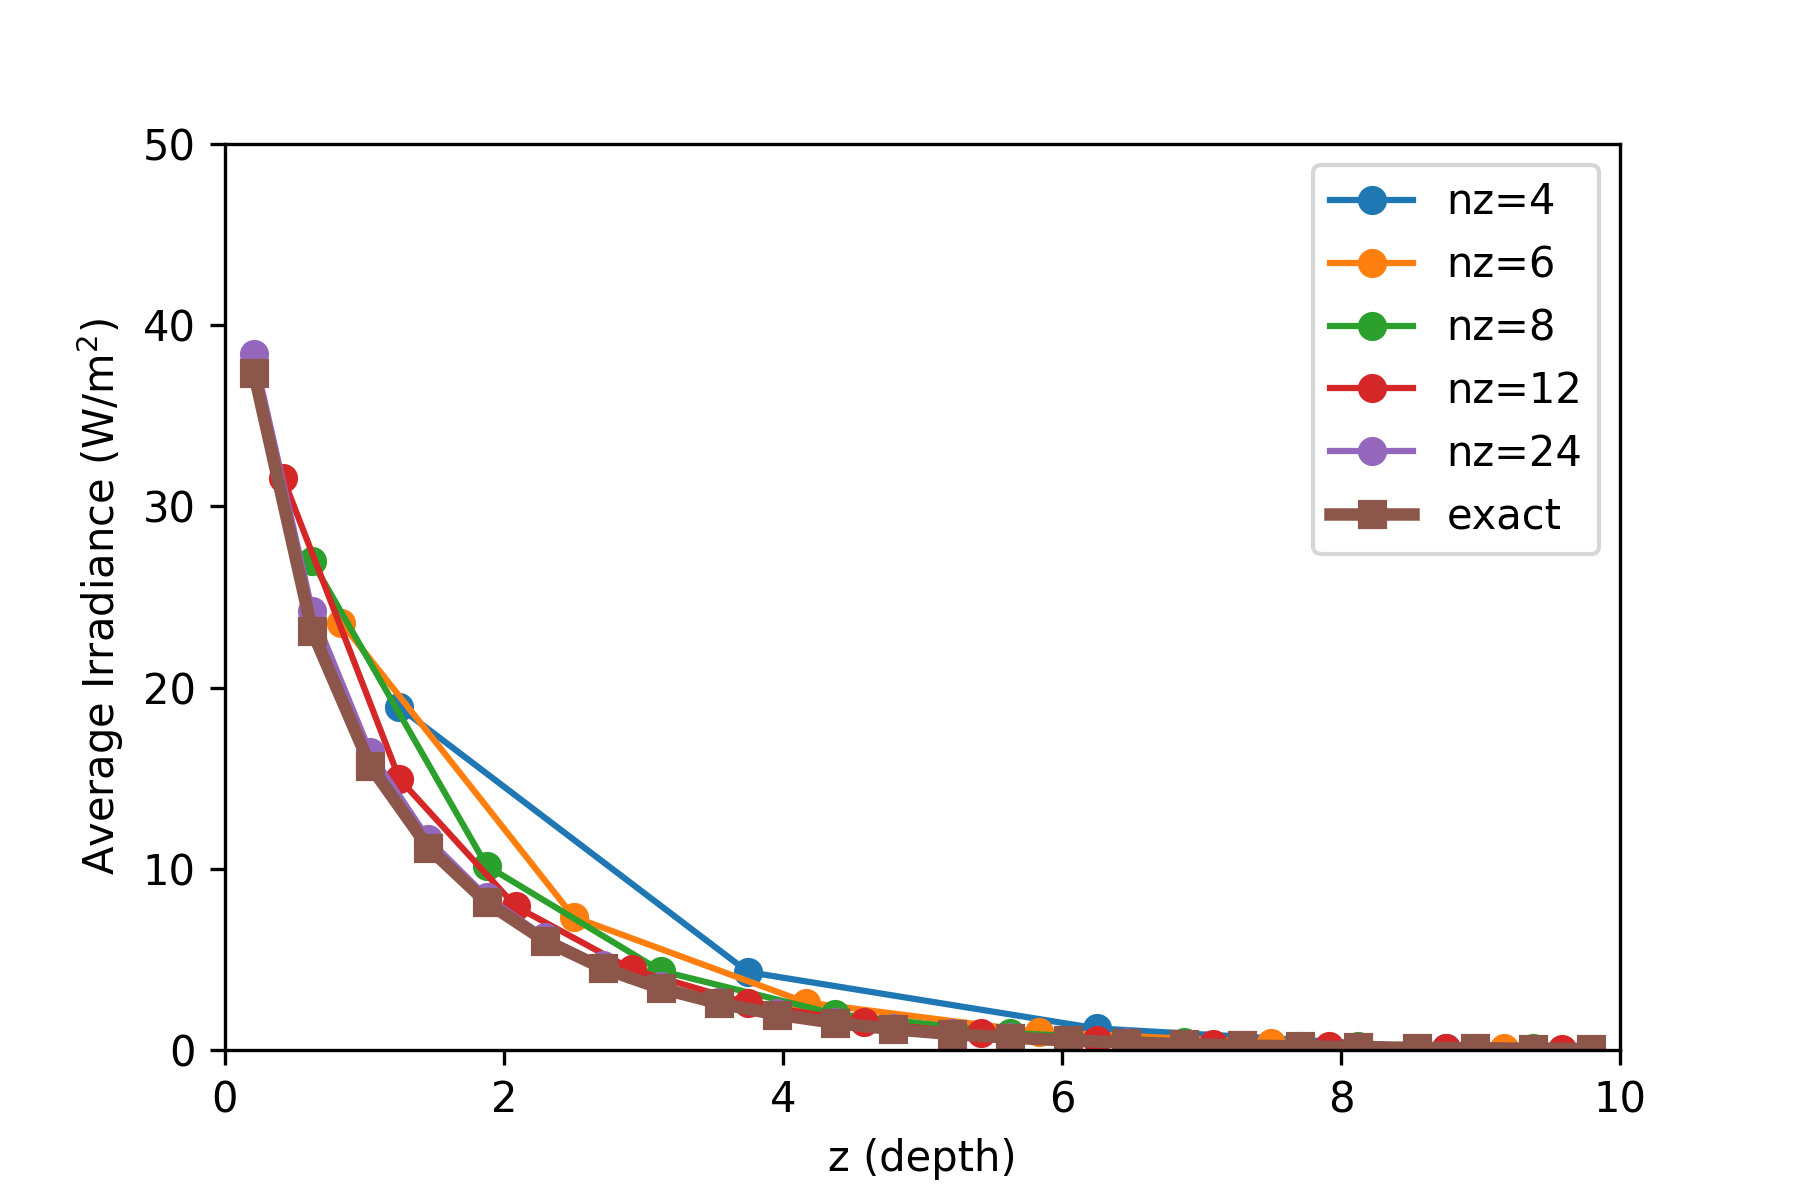
\includegraphics[width=4in]{exact_vs_fd_irrad}
  \caption{\DIFaddFL{Exact v.s. finite difference irradiance, linear scale}}
\end{figure}

\begin{figure}[H]
  \centering
  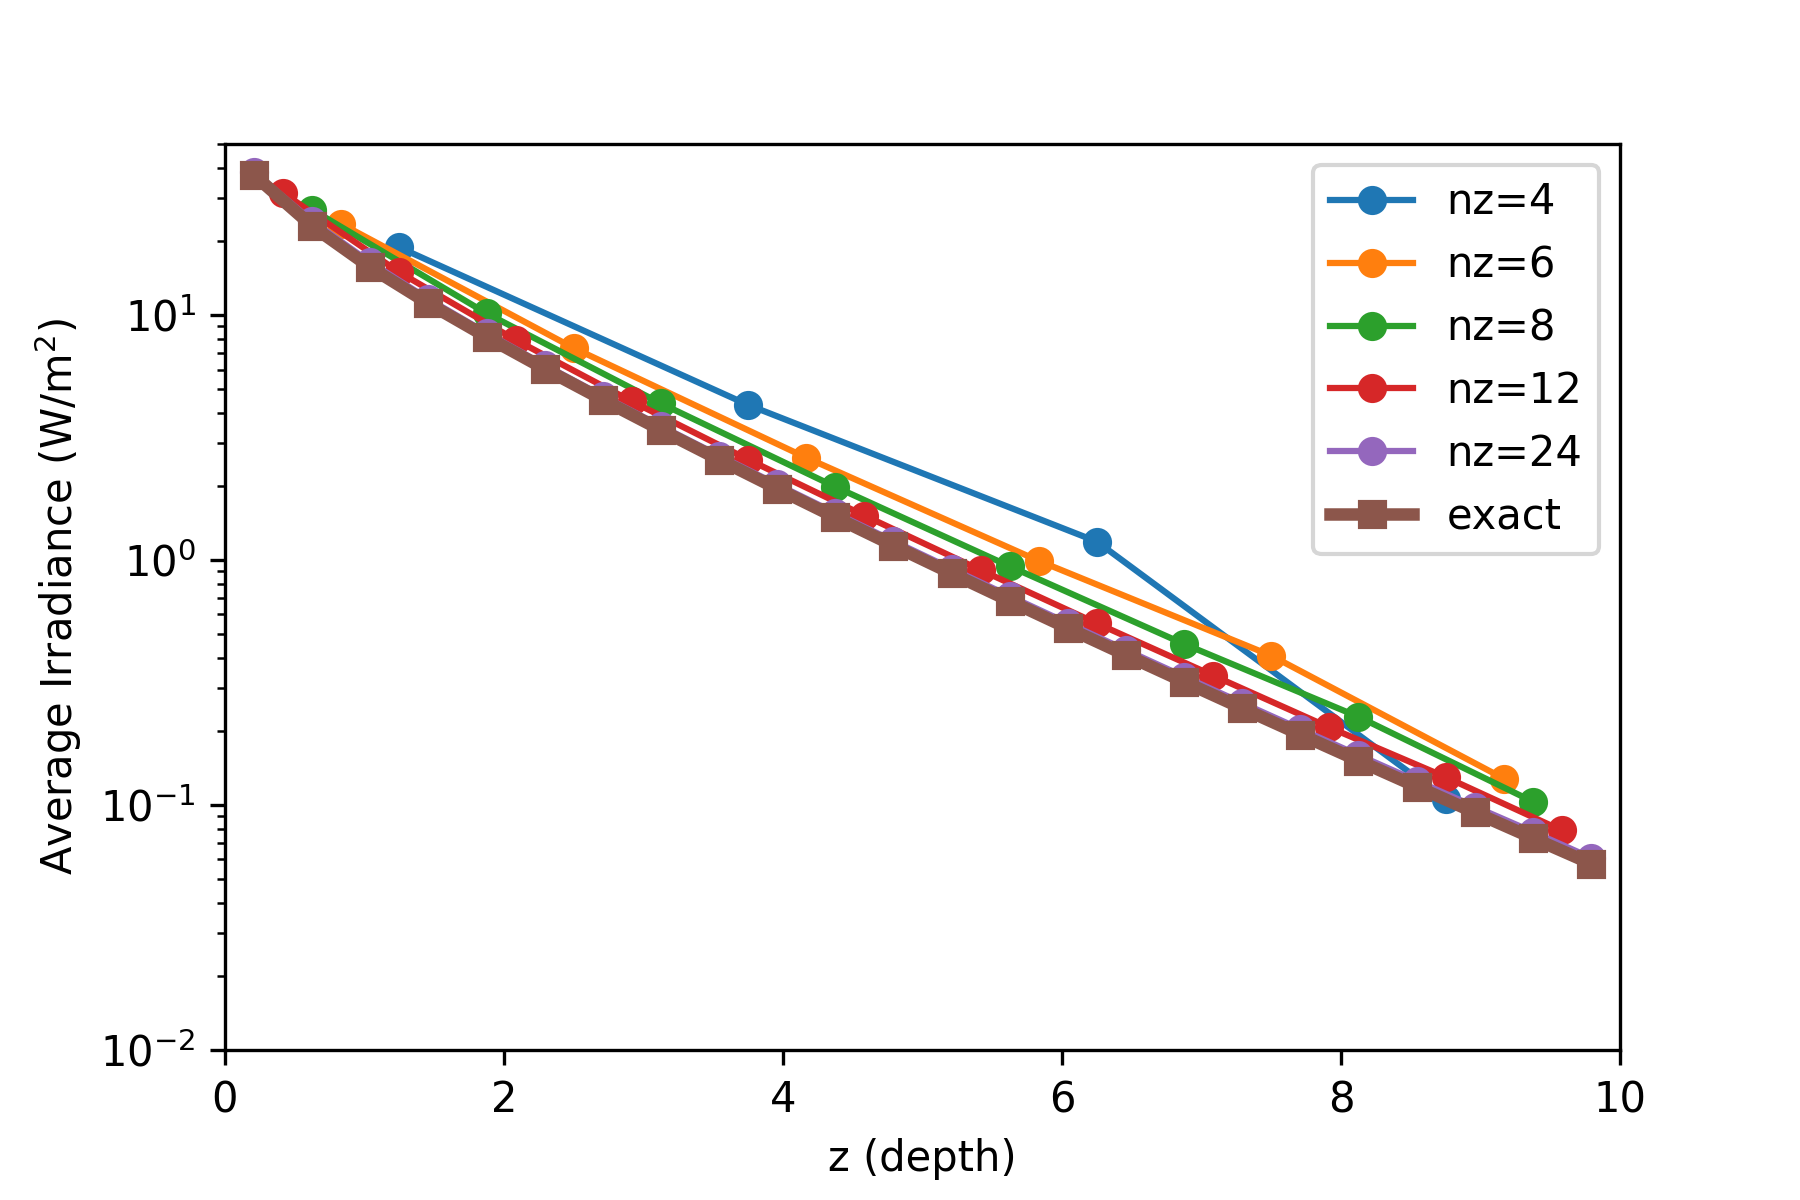
\includegraphics[width=4in]{exact_vs_fd_log_irrad}
  \caption{\DIFaddFL{Exact v.s. finite difference irradiance, log scale}}
\end{figure}

\begin{figure}[H]
  \centering
  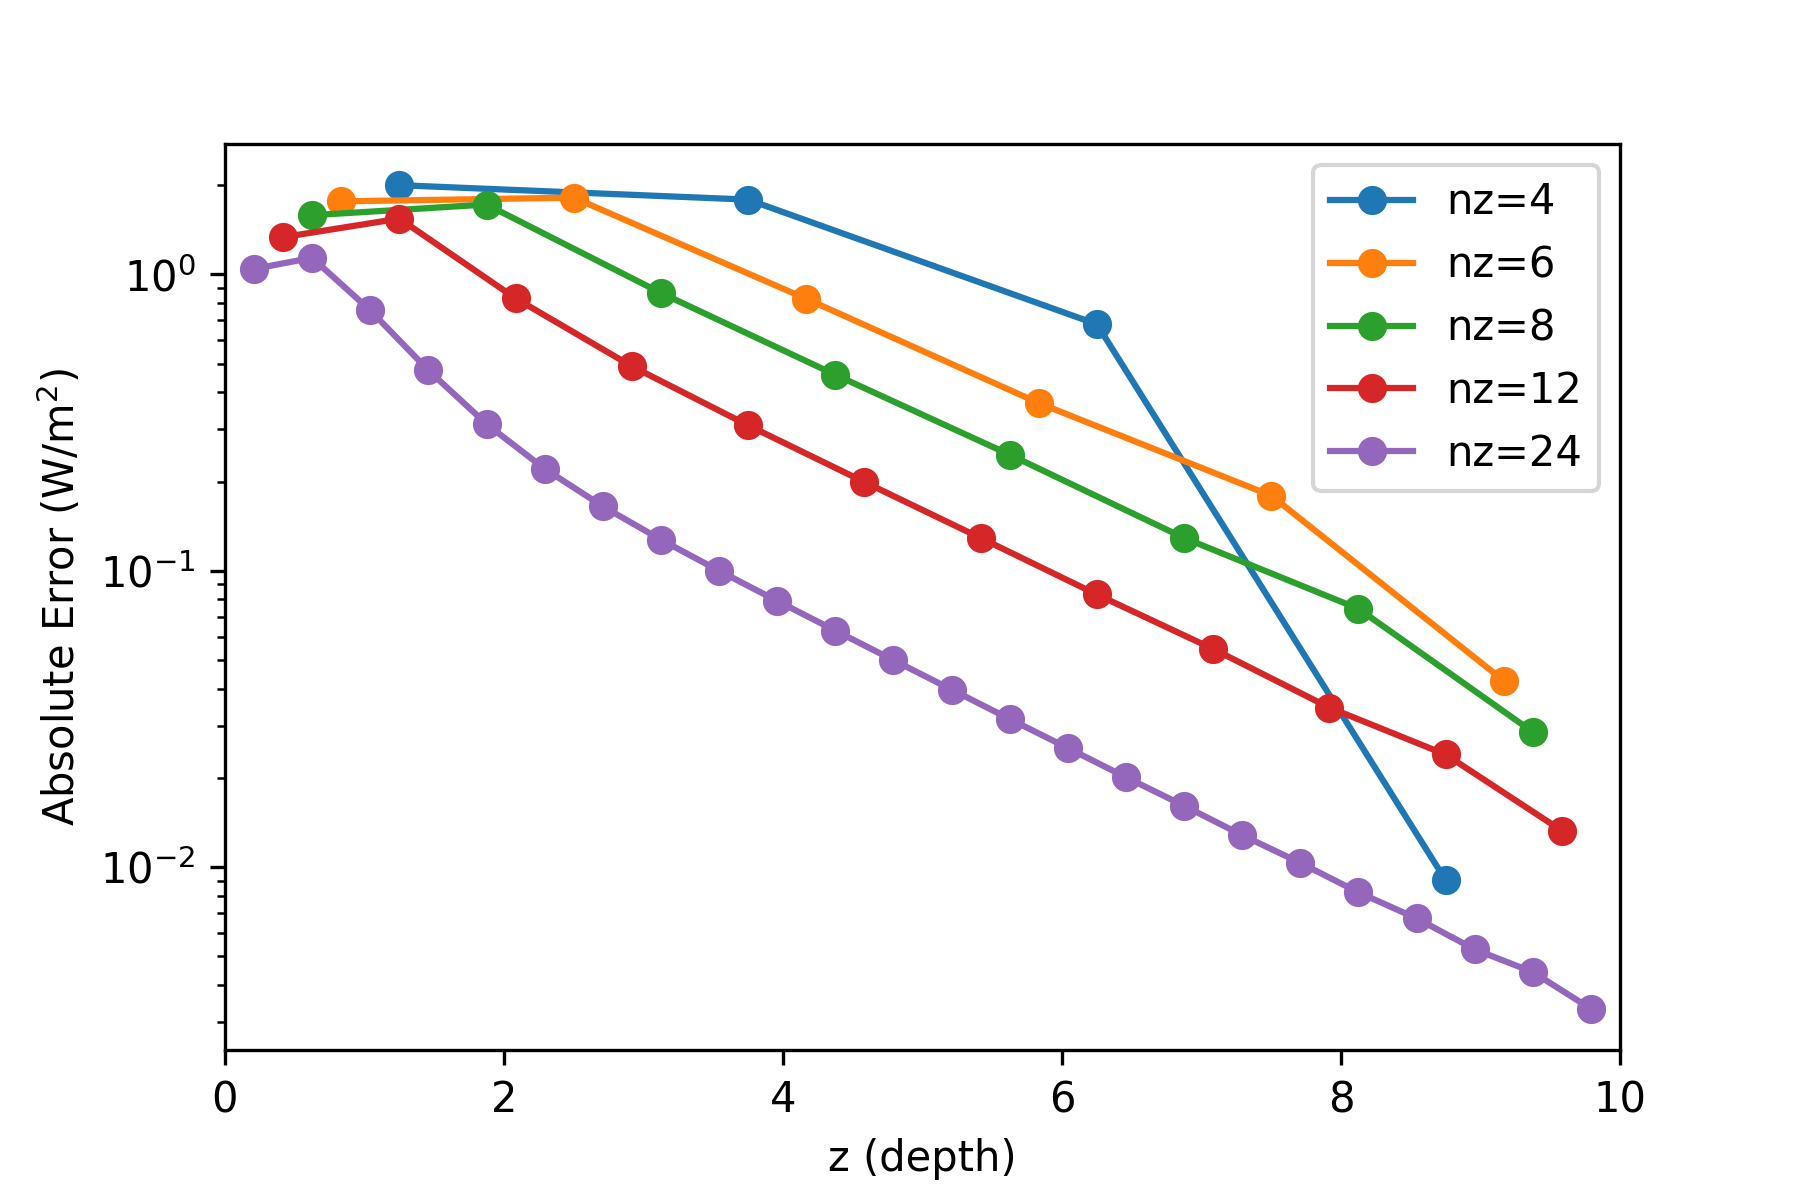
\includegraphics[width=4in]{exact_vs_fd_abs_err}
  \caption{\DIFaddFL{Exact v.s. finite difference irradiance, absolute error}}
\end{figure}

\begin{figure}[H]
  \centering
  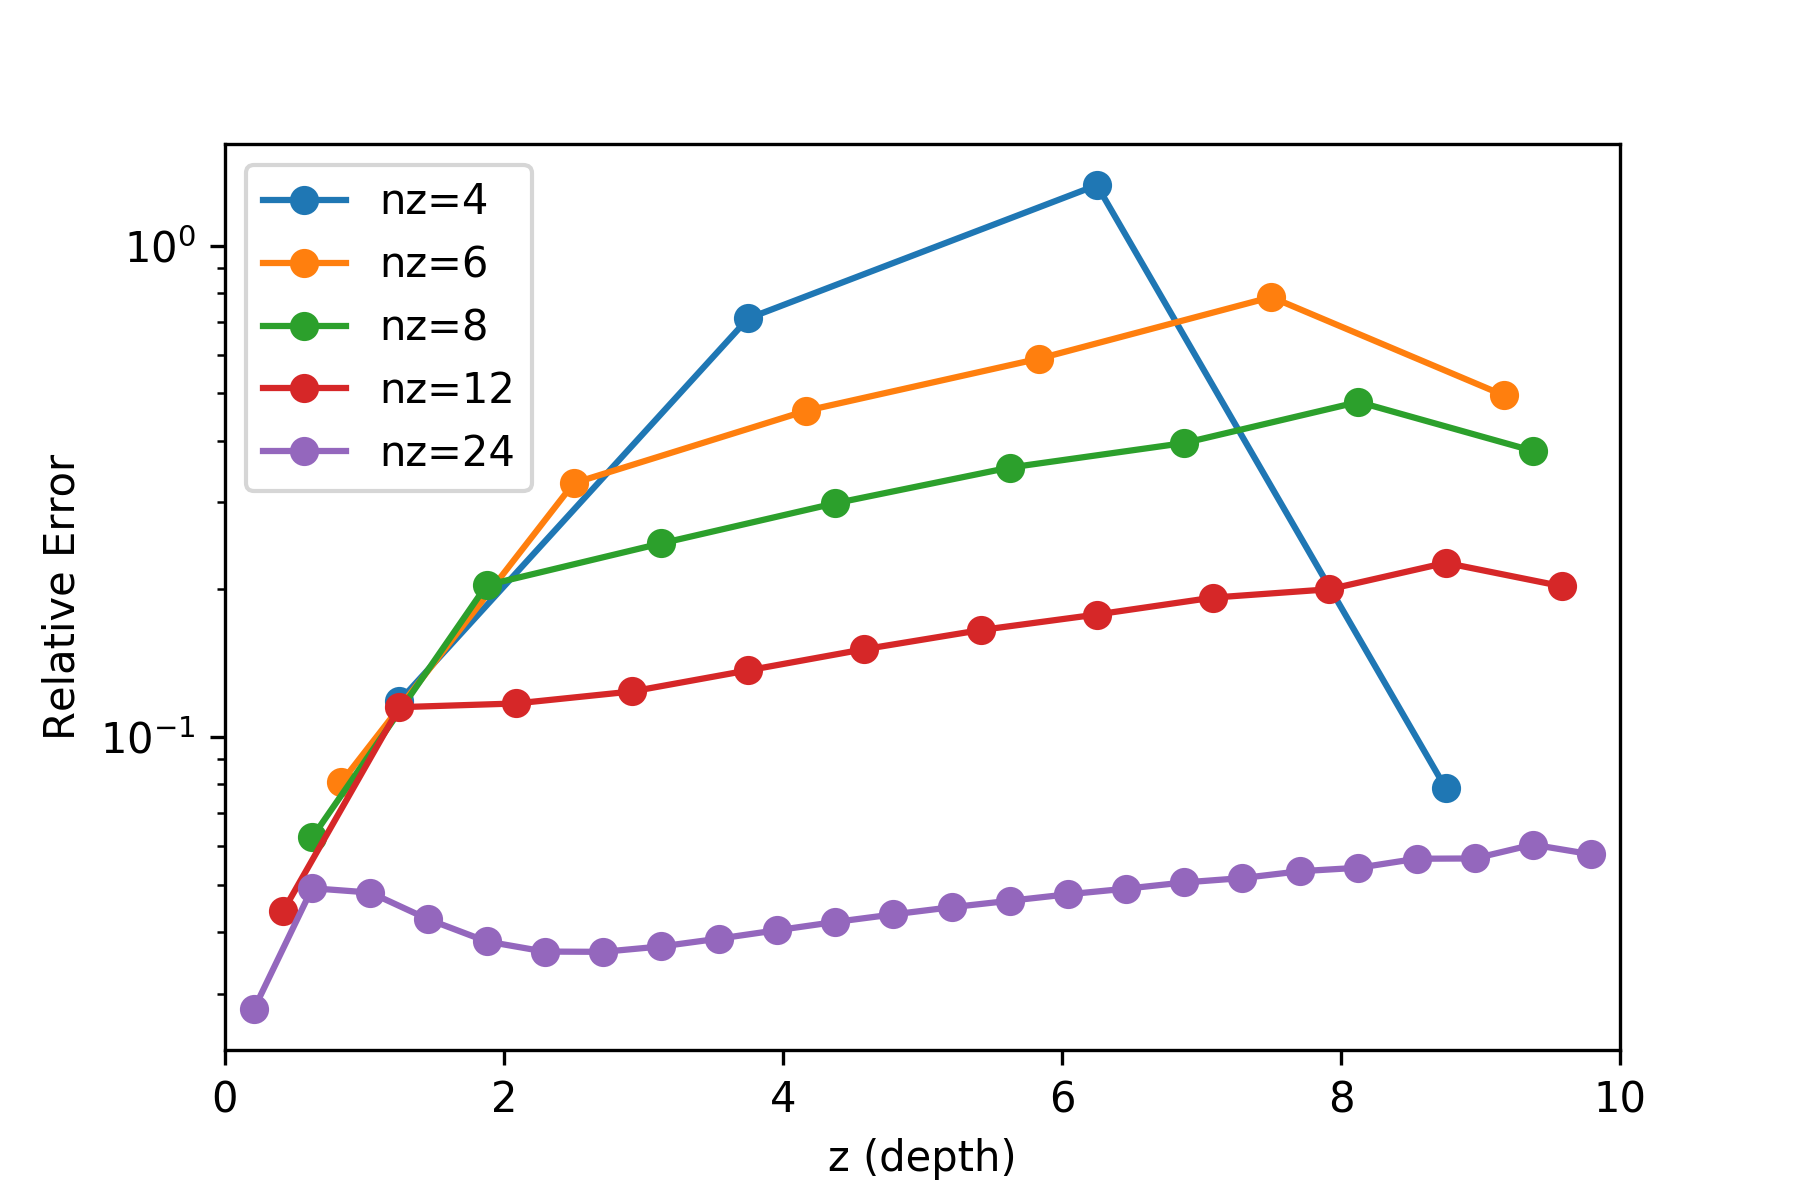
\includegraphics[width=4in]{exact_vs_fd_rel_err}
  \caption{\DIFaddFL{Exact v.s. finite difference irradiance, relative error}}
\end{figure}

\begin{figure}[H]
  \centering
  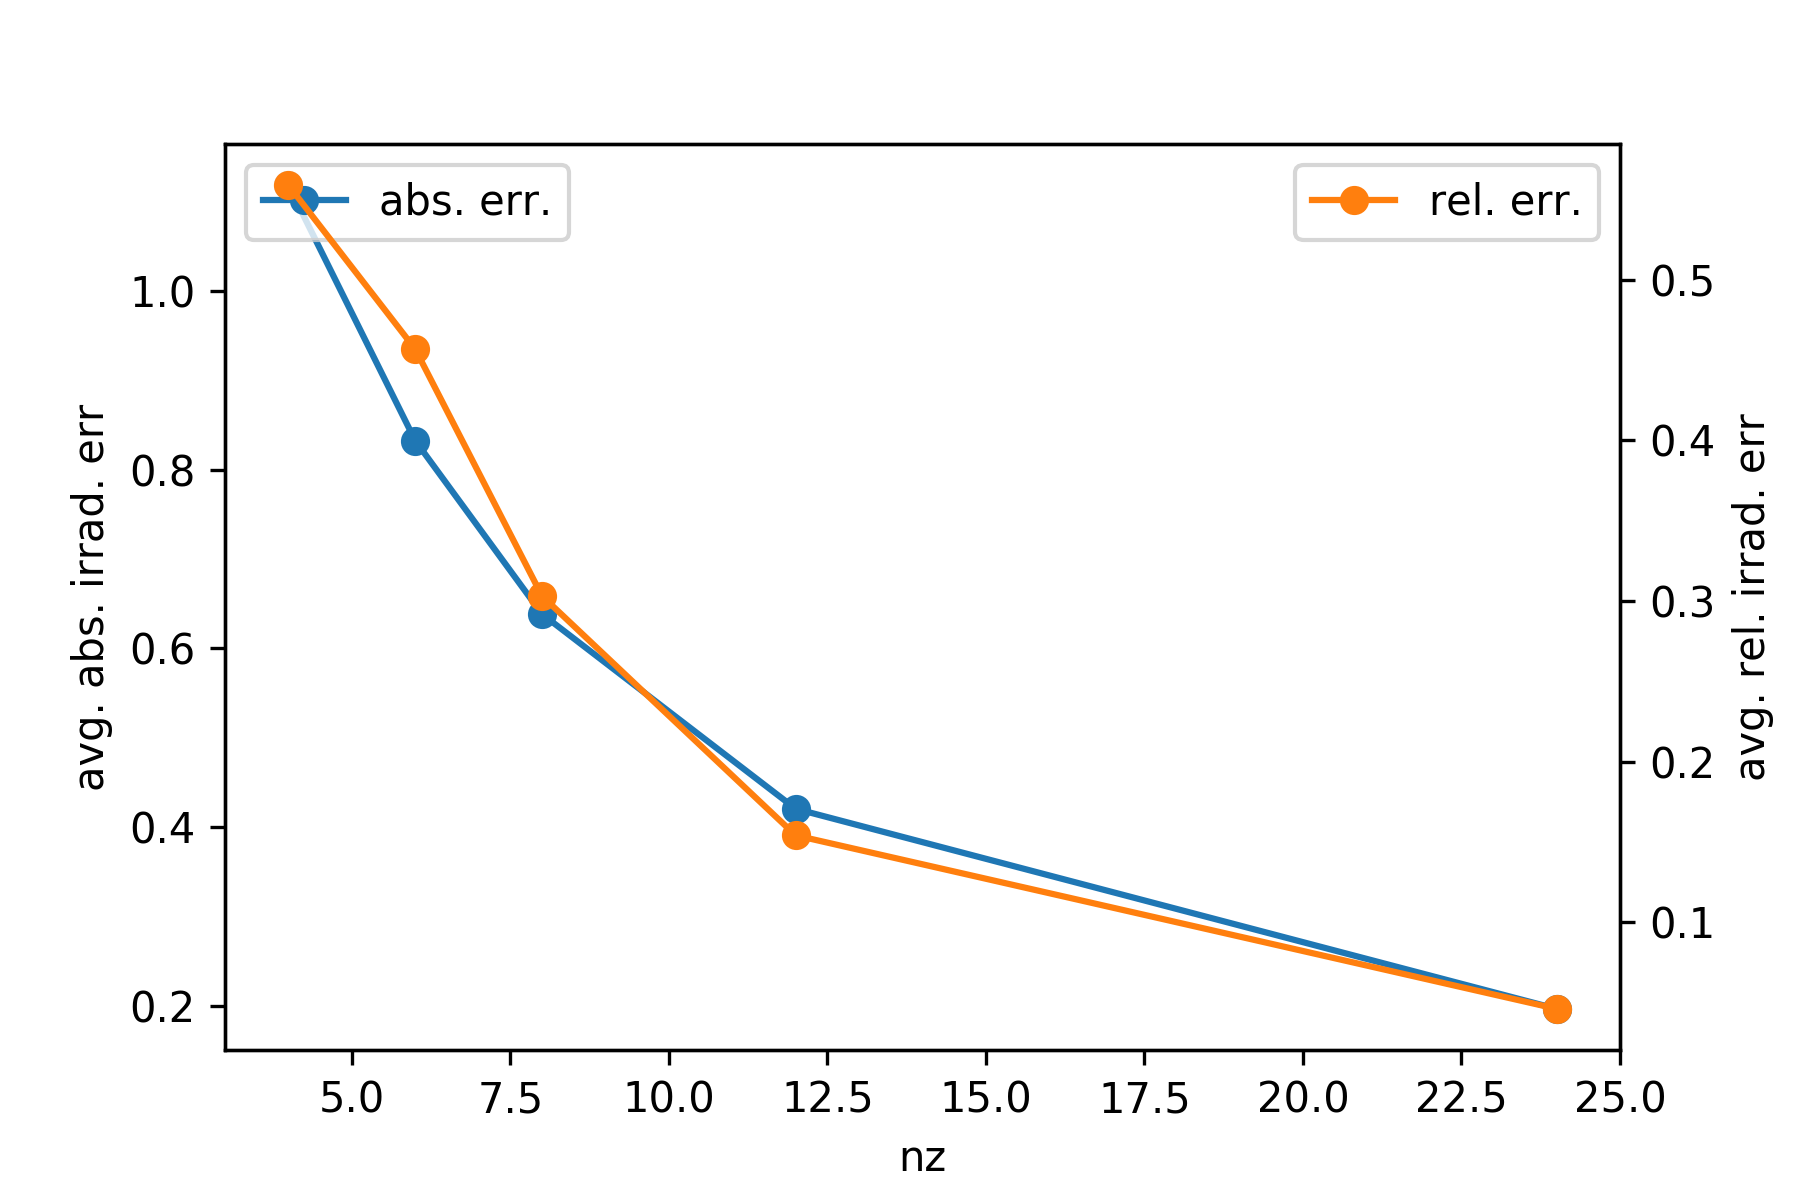
\includegraphics[width=4in]{exact_vs_fd_compare}
  \caption{\DIFaddFL{Exact v.s. finite difference irradiance, relative error v.s. grid resolution}}
\end{figure}

\section{\DIFadd{Grid Study}}
\DIFadd{A five dimensional $(x,y,x,\theta,\phi)$ resolution space is nontrivial to characterize.
For the sake of reducing dimensionality, we define generic spatial and angular resolutions
$n_s$ and $n_a$ such that $n_s=n_x=n_y$ and $n_a=n_\theta=n_\phi$.
Remaining is a three-dimensional resolution space, $(n_s,n_z,n_a)$.
Rather than perform calculations at every possible combination of resolutions in the space,
we choose a maximum resolution of $20 \times 20 \times 20$.
We hold two of the three resolutions at the maximum value while varying the third.
For example, Figure \ref{fig:gs_ns} compares $4 \times 20 \times 20$}\DIFaddend , \DIFaddbegin \DIFadd{$6 \times 20 \times 20$, $8 \times 20 \times 20$, etc.
The quantity that we compare is }\textit{\DIFadd{perceived irradiance}}\DIFadd{, which is not the simple average irradiance in each depth layer.
Rather, the average is weighted by the normalized spatial kelp distribution to determine the average irradiance experienced by the kelp population.
For more detail, see Section \ref{sec:perceived_irrad}
}

\DIFadd{Note the different natures of convergence in each dimension.
In varying $n_s$, we see that the accuracy is very low for small $n_s$ values.
This is because in these cases, the horizontal grid cells are too large to capture any detail
about the kelp fronds near the bottom where they are very small.
The kelp is effectively not present in these layers, and therefore the perceived irradiance is zero.
After increasing the resolution past this minimum threshold, however, little improvement results
from increasing $n_s$ further, as seen in Figure \ref{fig:gs_ns}.
On the other hand, Figure \ref{fig:gs_nz} shows that increasing the vertical resolution
consistently improves the accuracy of the solution.
Figure \ref{fig:gs_na} shows that $n_a$ is somewhere between the two,
demonstrating clear improvement with increasing resolution, though the improvement is not uniform over depth.
Figure \ref{fig:gs_compare} shows the trend of increasing accuracy with increasing resolution in each dimension.
}

\begin{figure}[H]
  \centering
  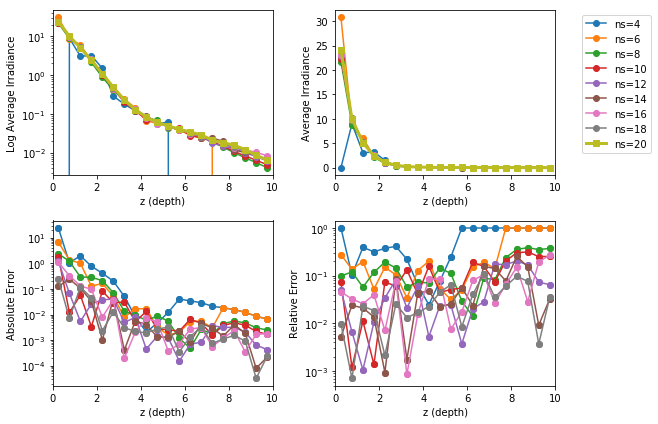
\includegraphics[width=5in]{gs_ns_20}
  \caption{\DIFaddFL{Grid study, $n_s$}}
  \label{fig:gs_ns}
\end{figure}

\begin{figure}[H]
  \centering
  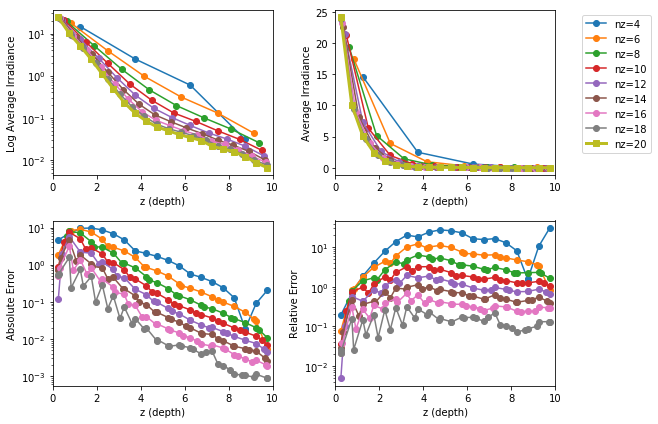
\includegraphics[width=5in]{gs_nz_20}
  \caption{\DIFaddFL{Grid study, $n_z$}}
  \label{fig:gs_nz}
\end{figure}

\begin{figure}[H]
  \centering
  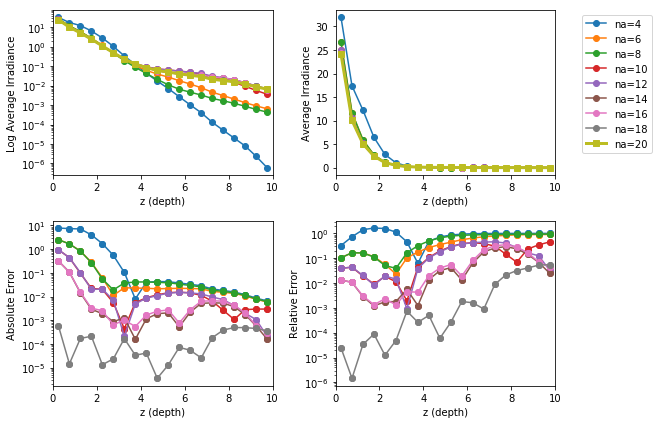
\includegraphics[width=5in]{gs_na_20}
  \caption{\DIFaddFL{Grid study, $n_a$}}
  \label{fig:gs_na}
\end{figure}

\begin{figure}[H]
  \centering
  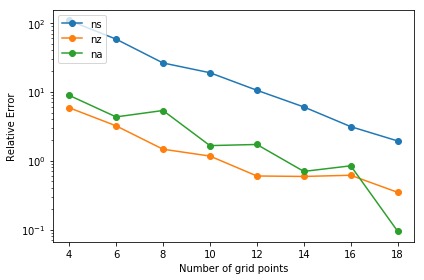
\includegraphics[width=5in]{gs_20}
  \caption{\DIFaddFL{Grid study, summary}}
  \label{fig:gs_compare}
\end{figure}


\section{\DIFadd{Asymptotic Convergence}}
\label{sec:asym_conv}

\DIFadd{In this section, the four water cases from Table \ref{tab:petzold} are considered.
In each case, the full finite difference solution is calculated on an $18 \times 18 \times 18$ grid,
and asymptotic approximations are given, varying the number of terms used in the asymptotic series.
Perceived irradiances are shown, }\DIFaddend as well as \DIFdelbegin \DIFdel{average irradance over depth}\DIFdelend \DIFaddbegin \DIFadd{errors from the finite difference solution}\DIFaddend .

\DIFdelbegin \DIFdel{- absorption coefficient}\DIFdelend \DIFaddbegin \DIFadd{In the first two cases, when the scattering coefficient is the same order or smaller as the absorption coefficient,
the asymptotic approximation converges to the finite difference solution.
However, in the very turbid water of the San Diego Harbor, the scattering coefficient is an order of magnitude higher
than the absorption coefficient, causing the asymptotic solution to quickly diverge.
In figure \ref{fig:asym_conv_compare}, average relative errors for the two converging cases are shown.
In both cases, the accuracy improves with more scattering events until it plateaus.
In the first case, 4 scattering events is sufficient, whereas in the second, the accuracy improves until 12 scattering events.
}\DIFaddend 

\DIFdelbegin \DIFdel{- scattering coefficient }\DIFdelend \DIFaddbegin \begin{figure}[H]
  \centering
  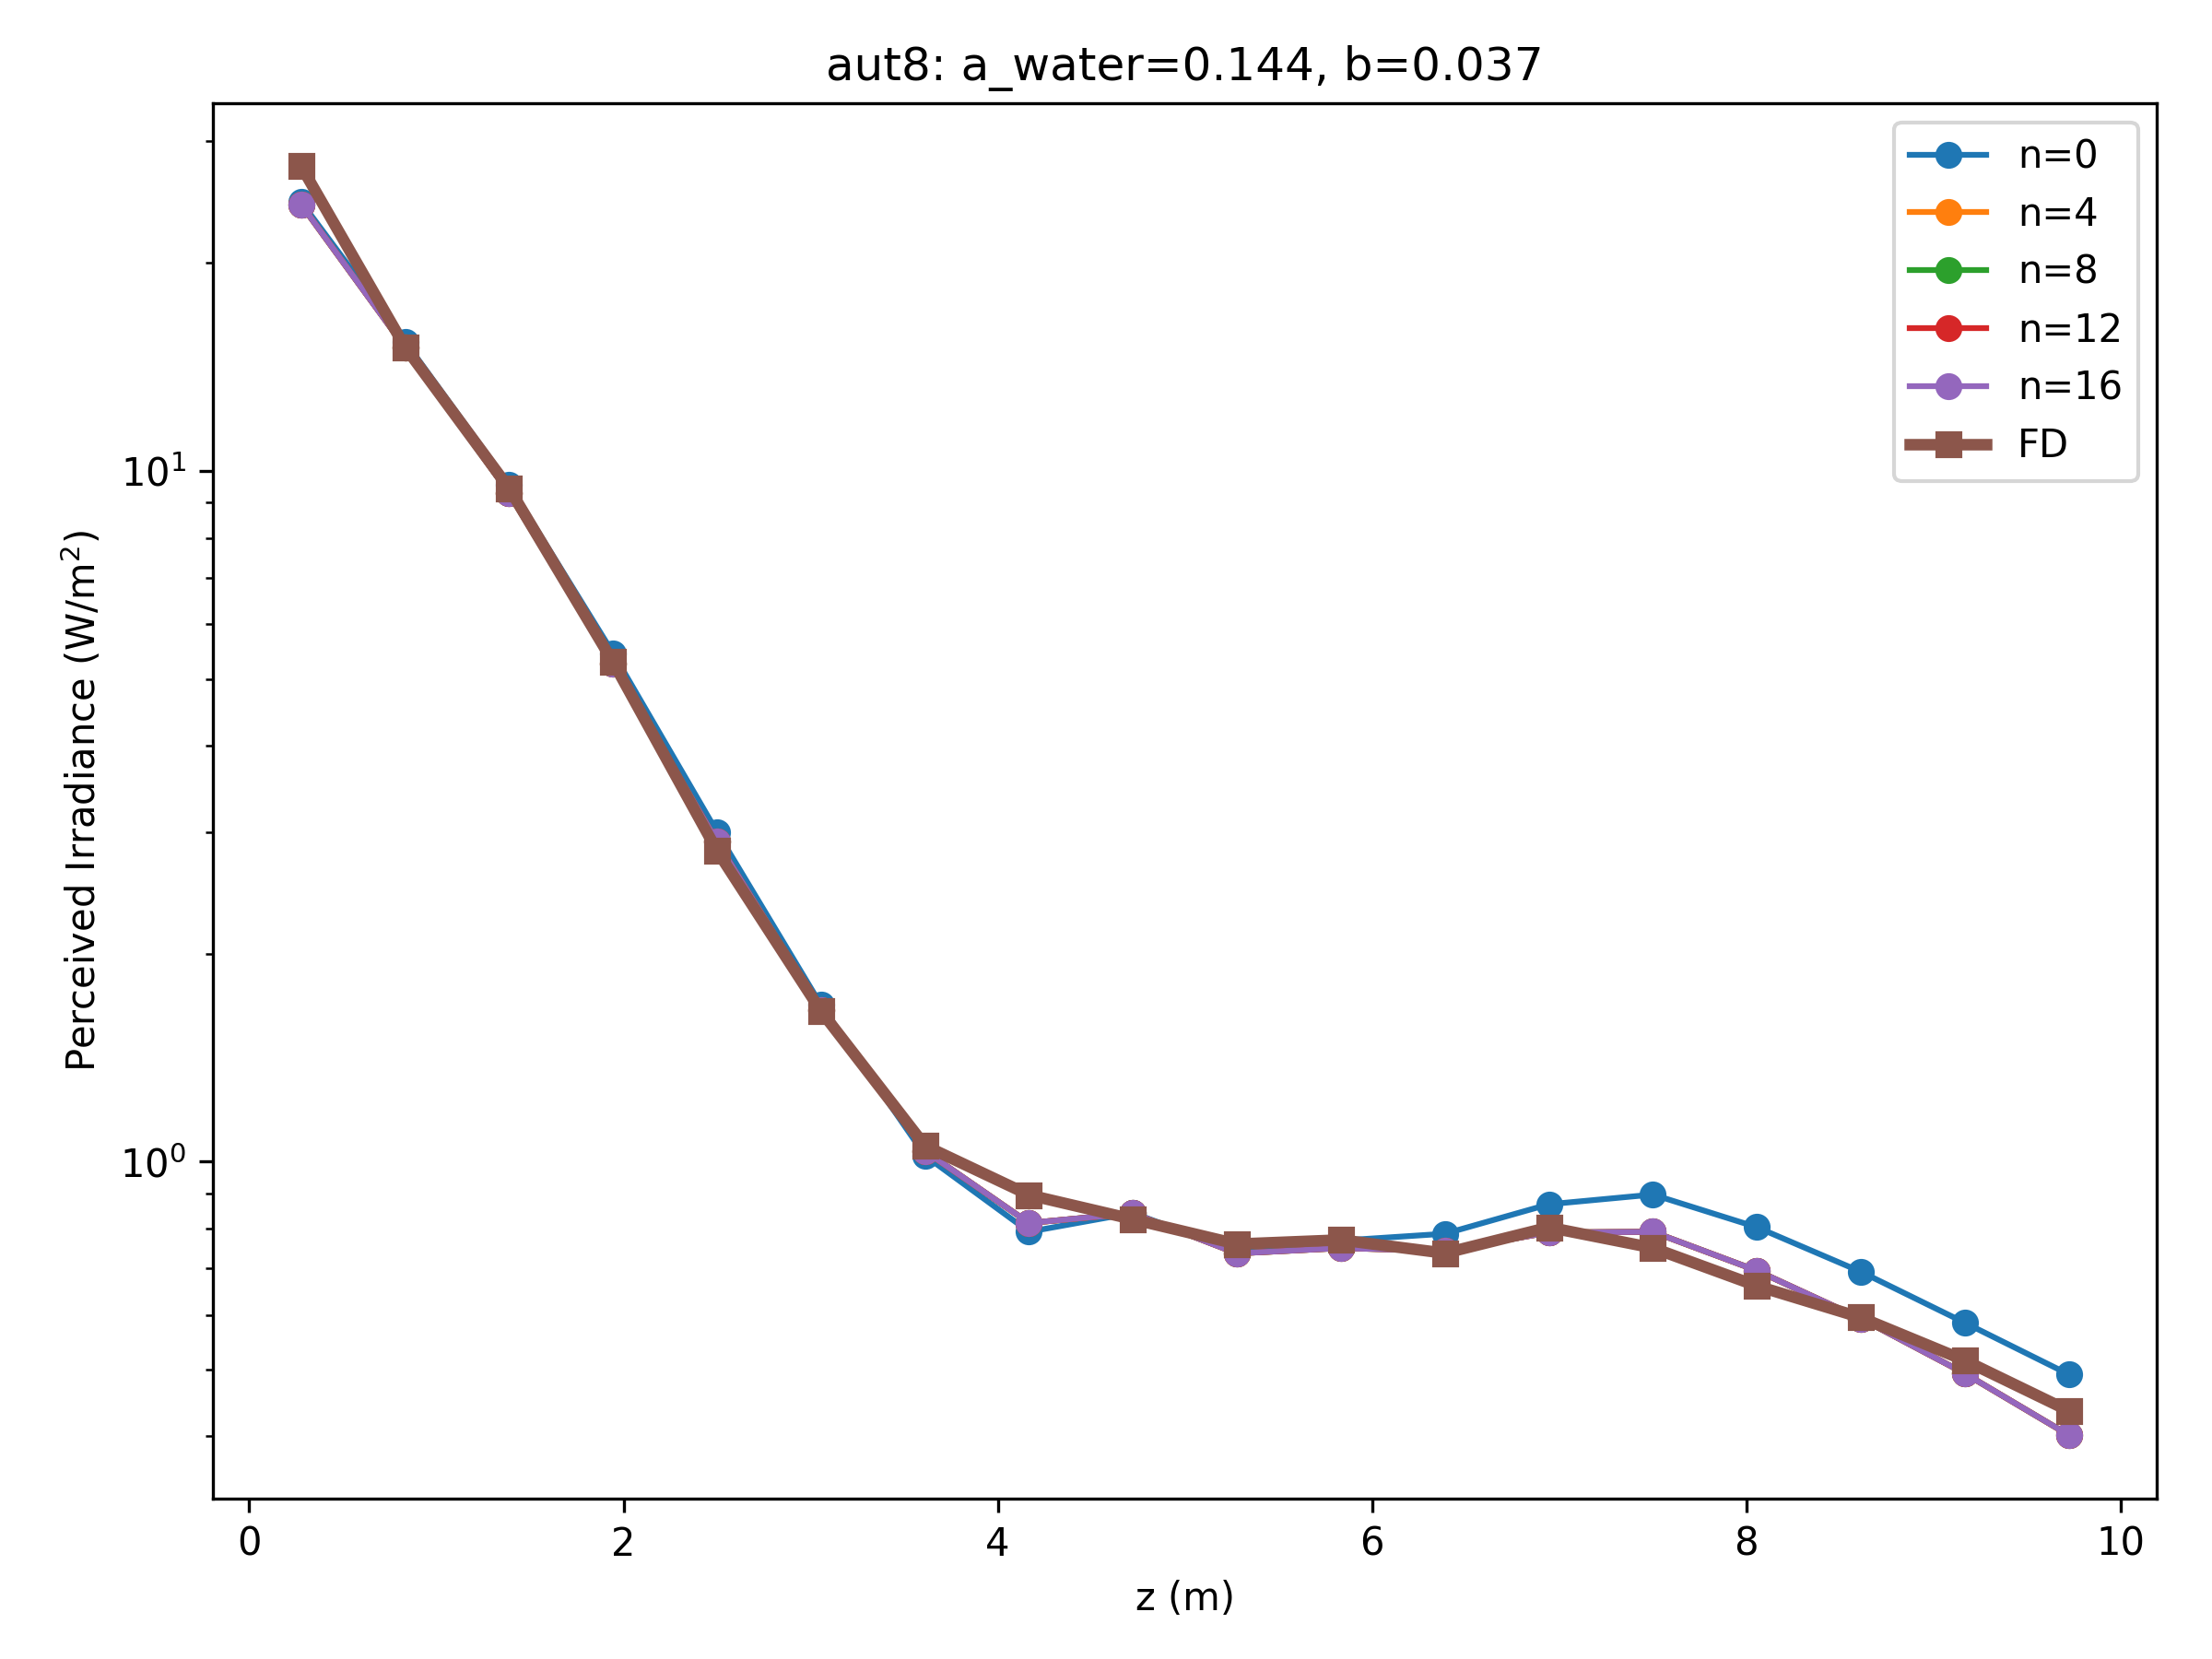
\includegraphics[width=4in]{asym_conv_irrad_aut8}
  \caption{\DIFaddFL{Successive asymptotic approximations, irradiance: }\texttt{\DIFaddFL{AUT8}}}
\end{figure}
\DIFaddend 

\DIFdelbegin \DIFdel{- VSF
}\DIFdelend \DIFaddbegin \begin{figure}[H]
  \centering
  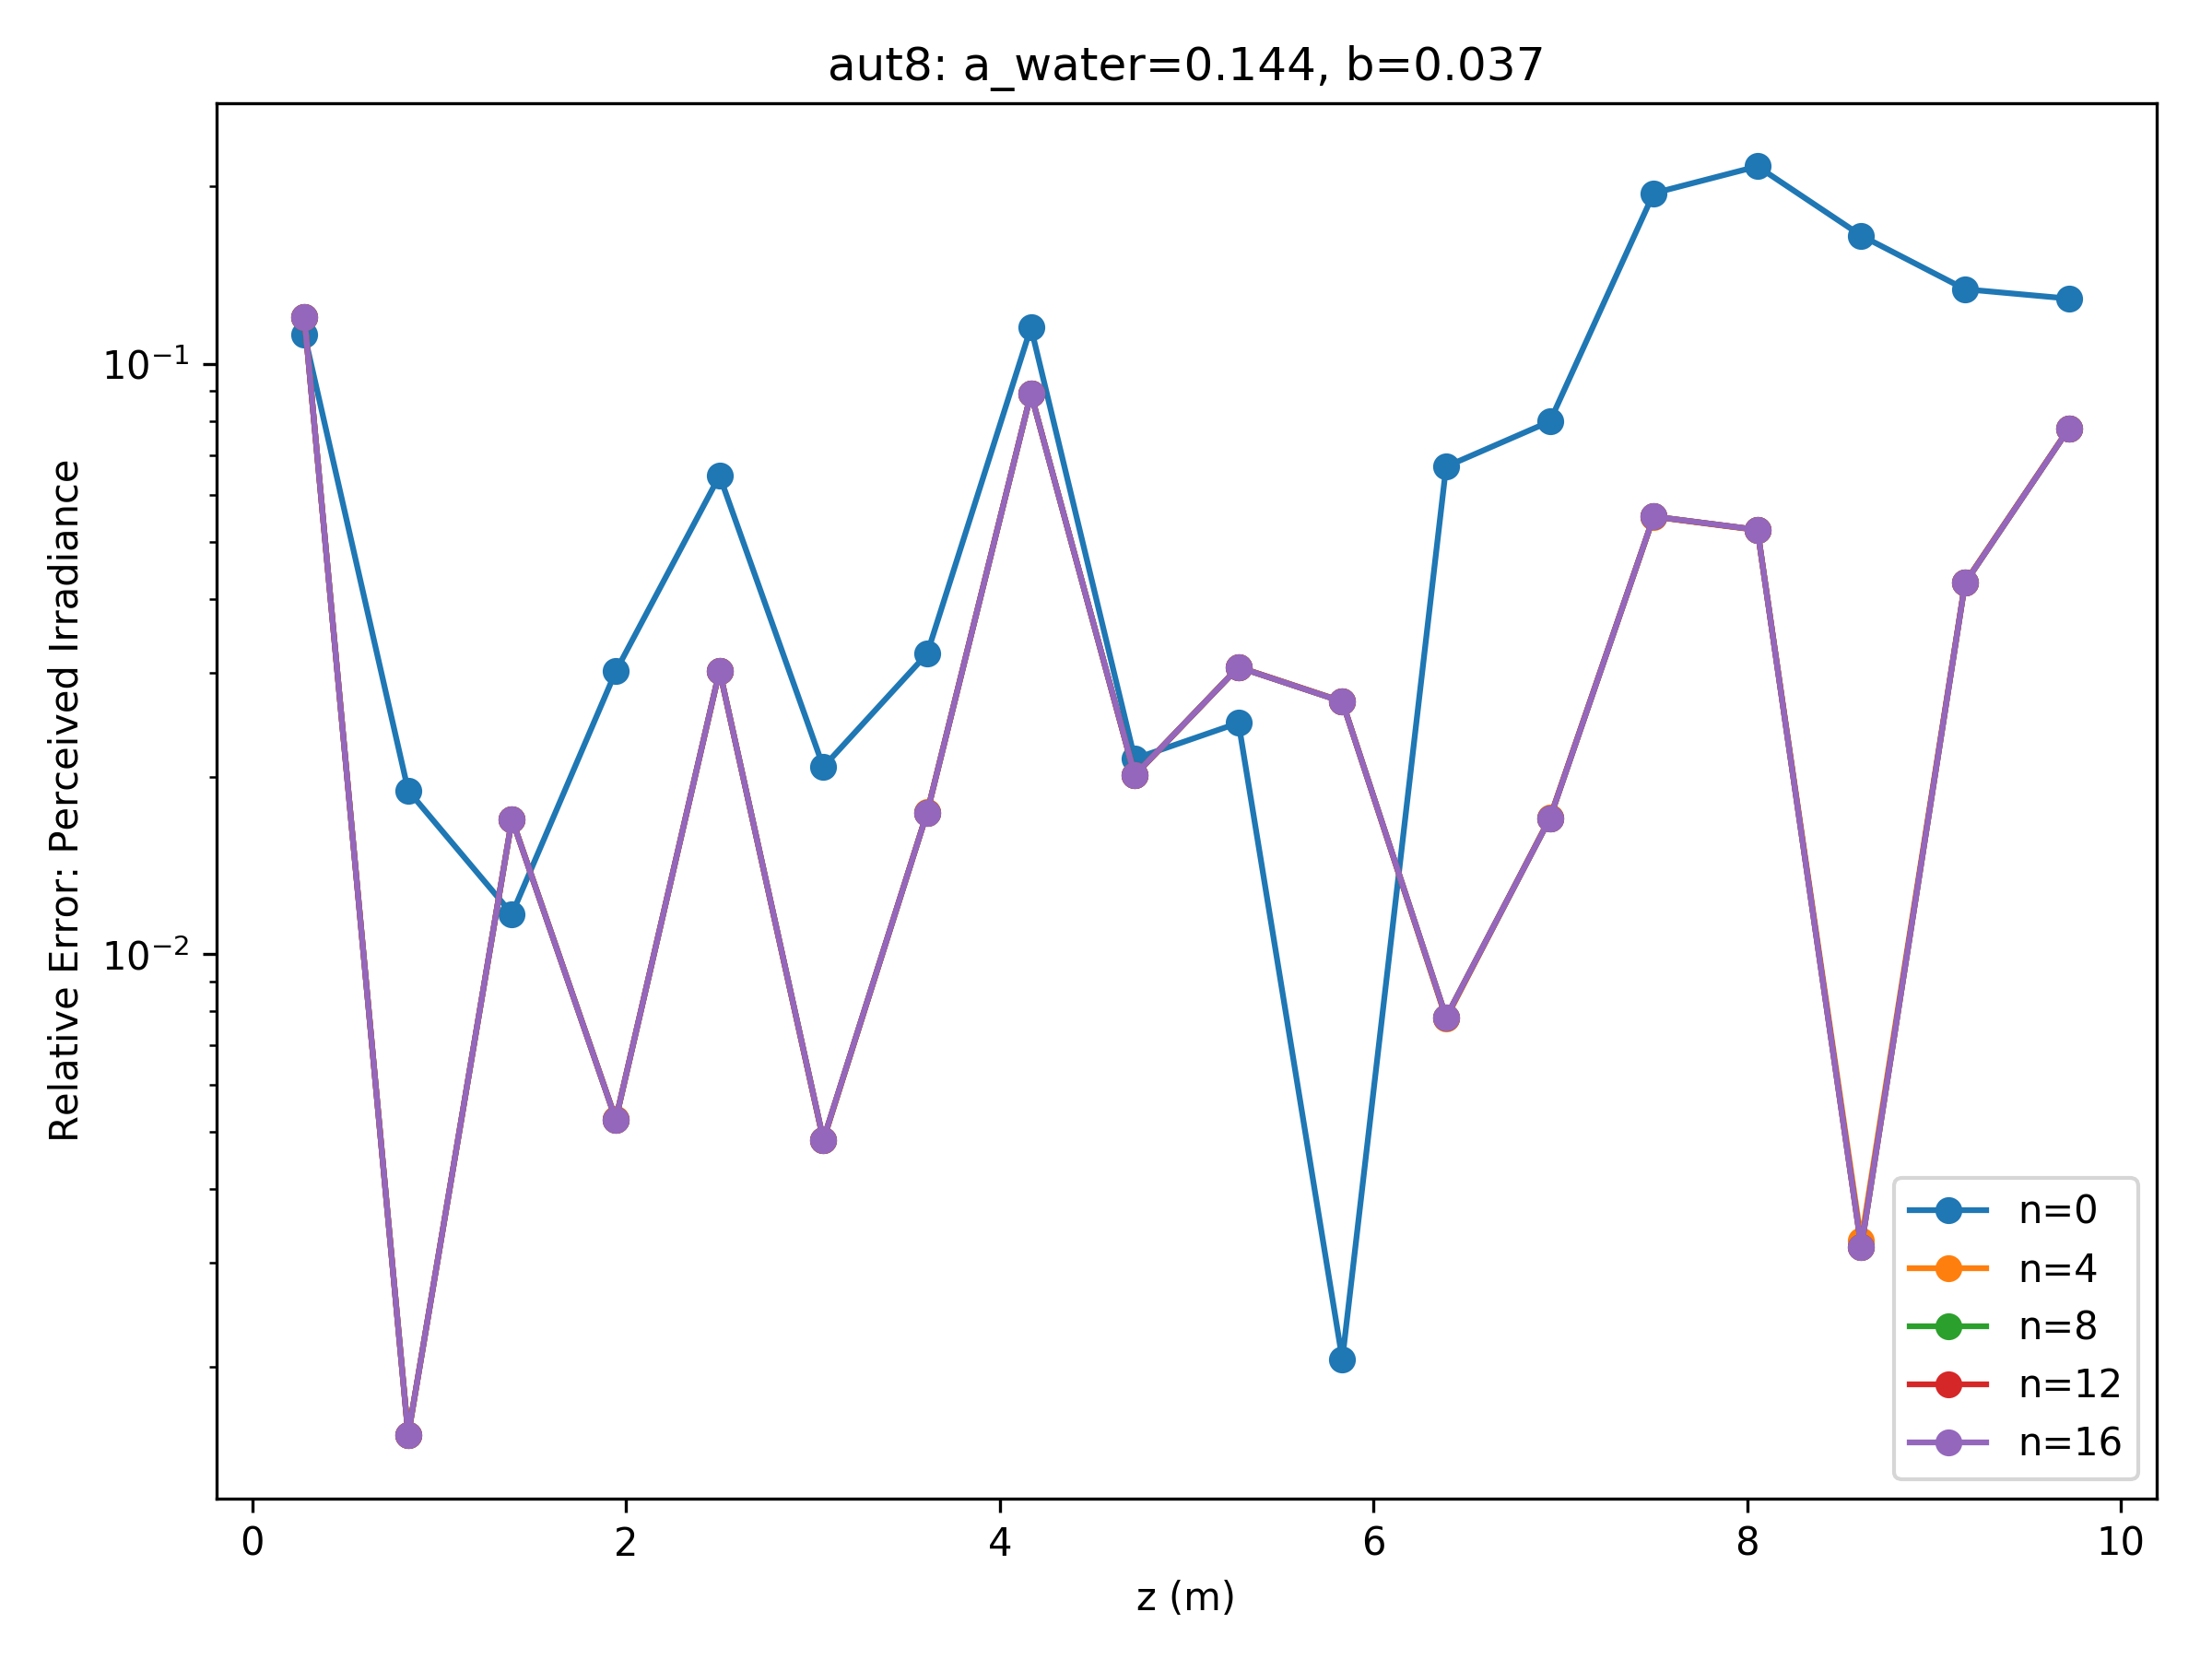
\includegraphics[width=4in]{asym_conv_rel_err_aut8}
  \caption{\DIFaddFL{Successive asymptotic approximations, relative error: }\texttt{\DIFaddFL{AUT8}}}
\end{figure}
\DIFaddend 


\DIFdelbegin \DIFdel{- frond bending coefficient
}\DIFdelend \DIFaddbegin \begin{figure}[H]
  \centering
  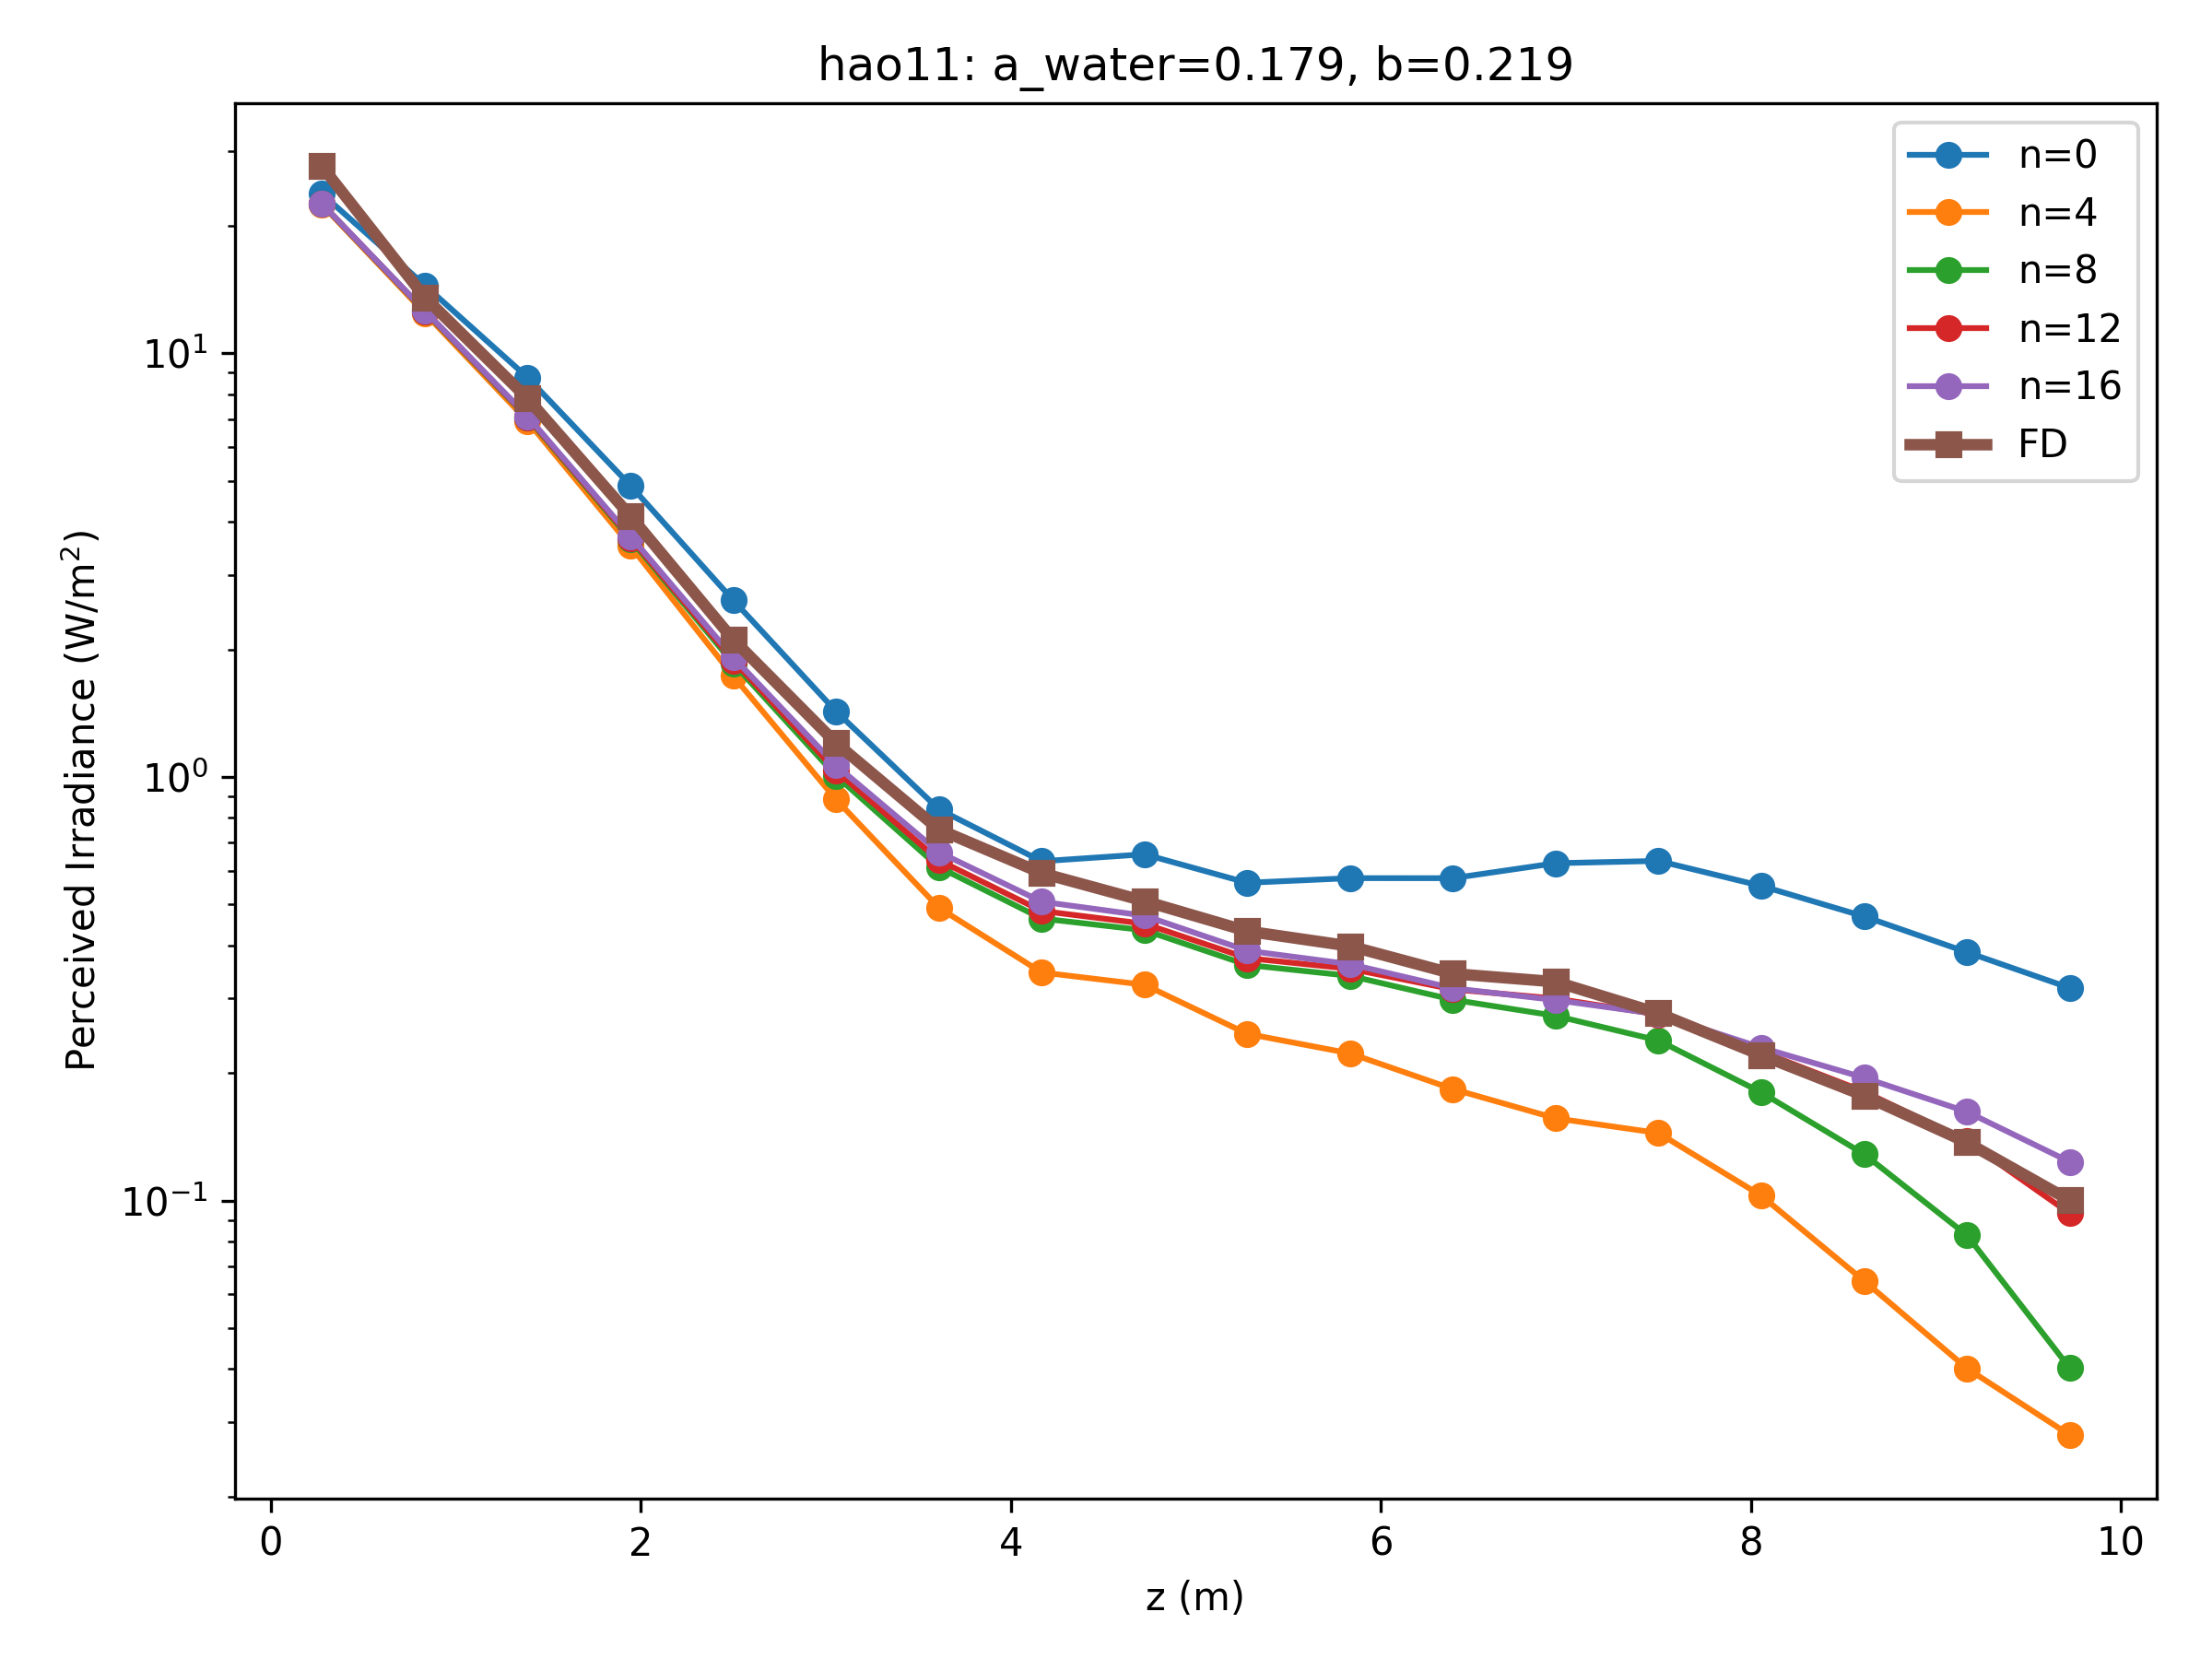
\includegraphics[width=4in]{asym_conv_irrad_hao11}
  \caption{\DIFaddFL{Successive asymptotic approximations, irradiance: }\texttt{\DIFaddFL{HAO11}}}
\end{figure}
\DIFaddend 

\DIFdelbegin \section{\DIFdel{Kelp Cultivation Simulation}}
%DIFAUXCMD
\addtocounter{section}{-1}%DIFAUXCMD
\DIFdelend \DIFaddbegin \begin{figure}[H]
  \centering
  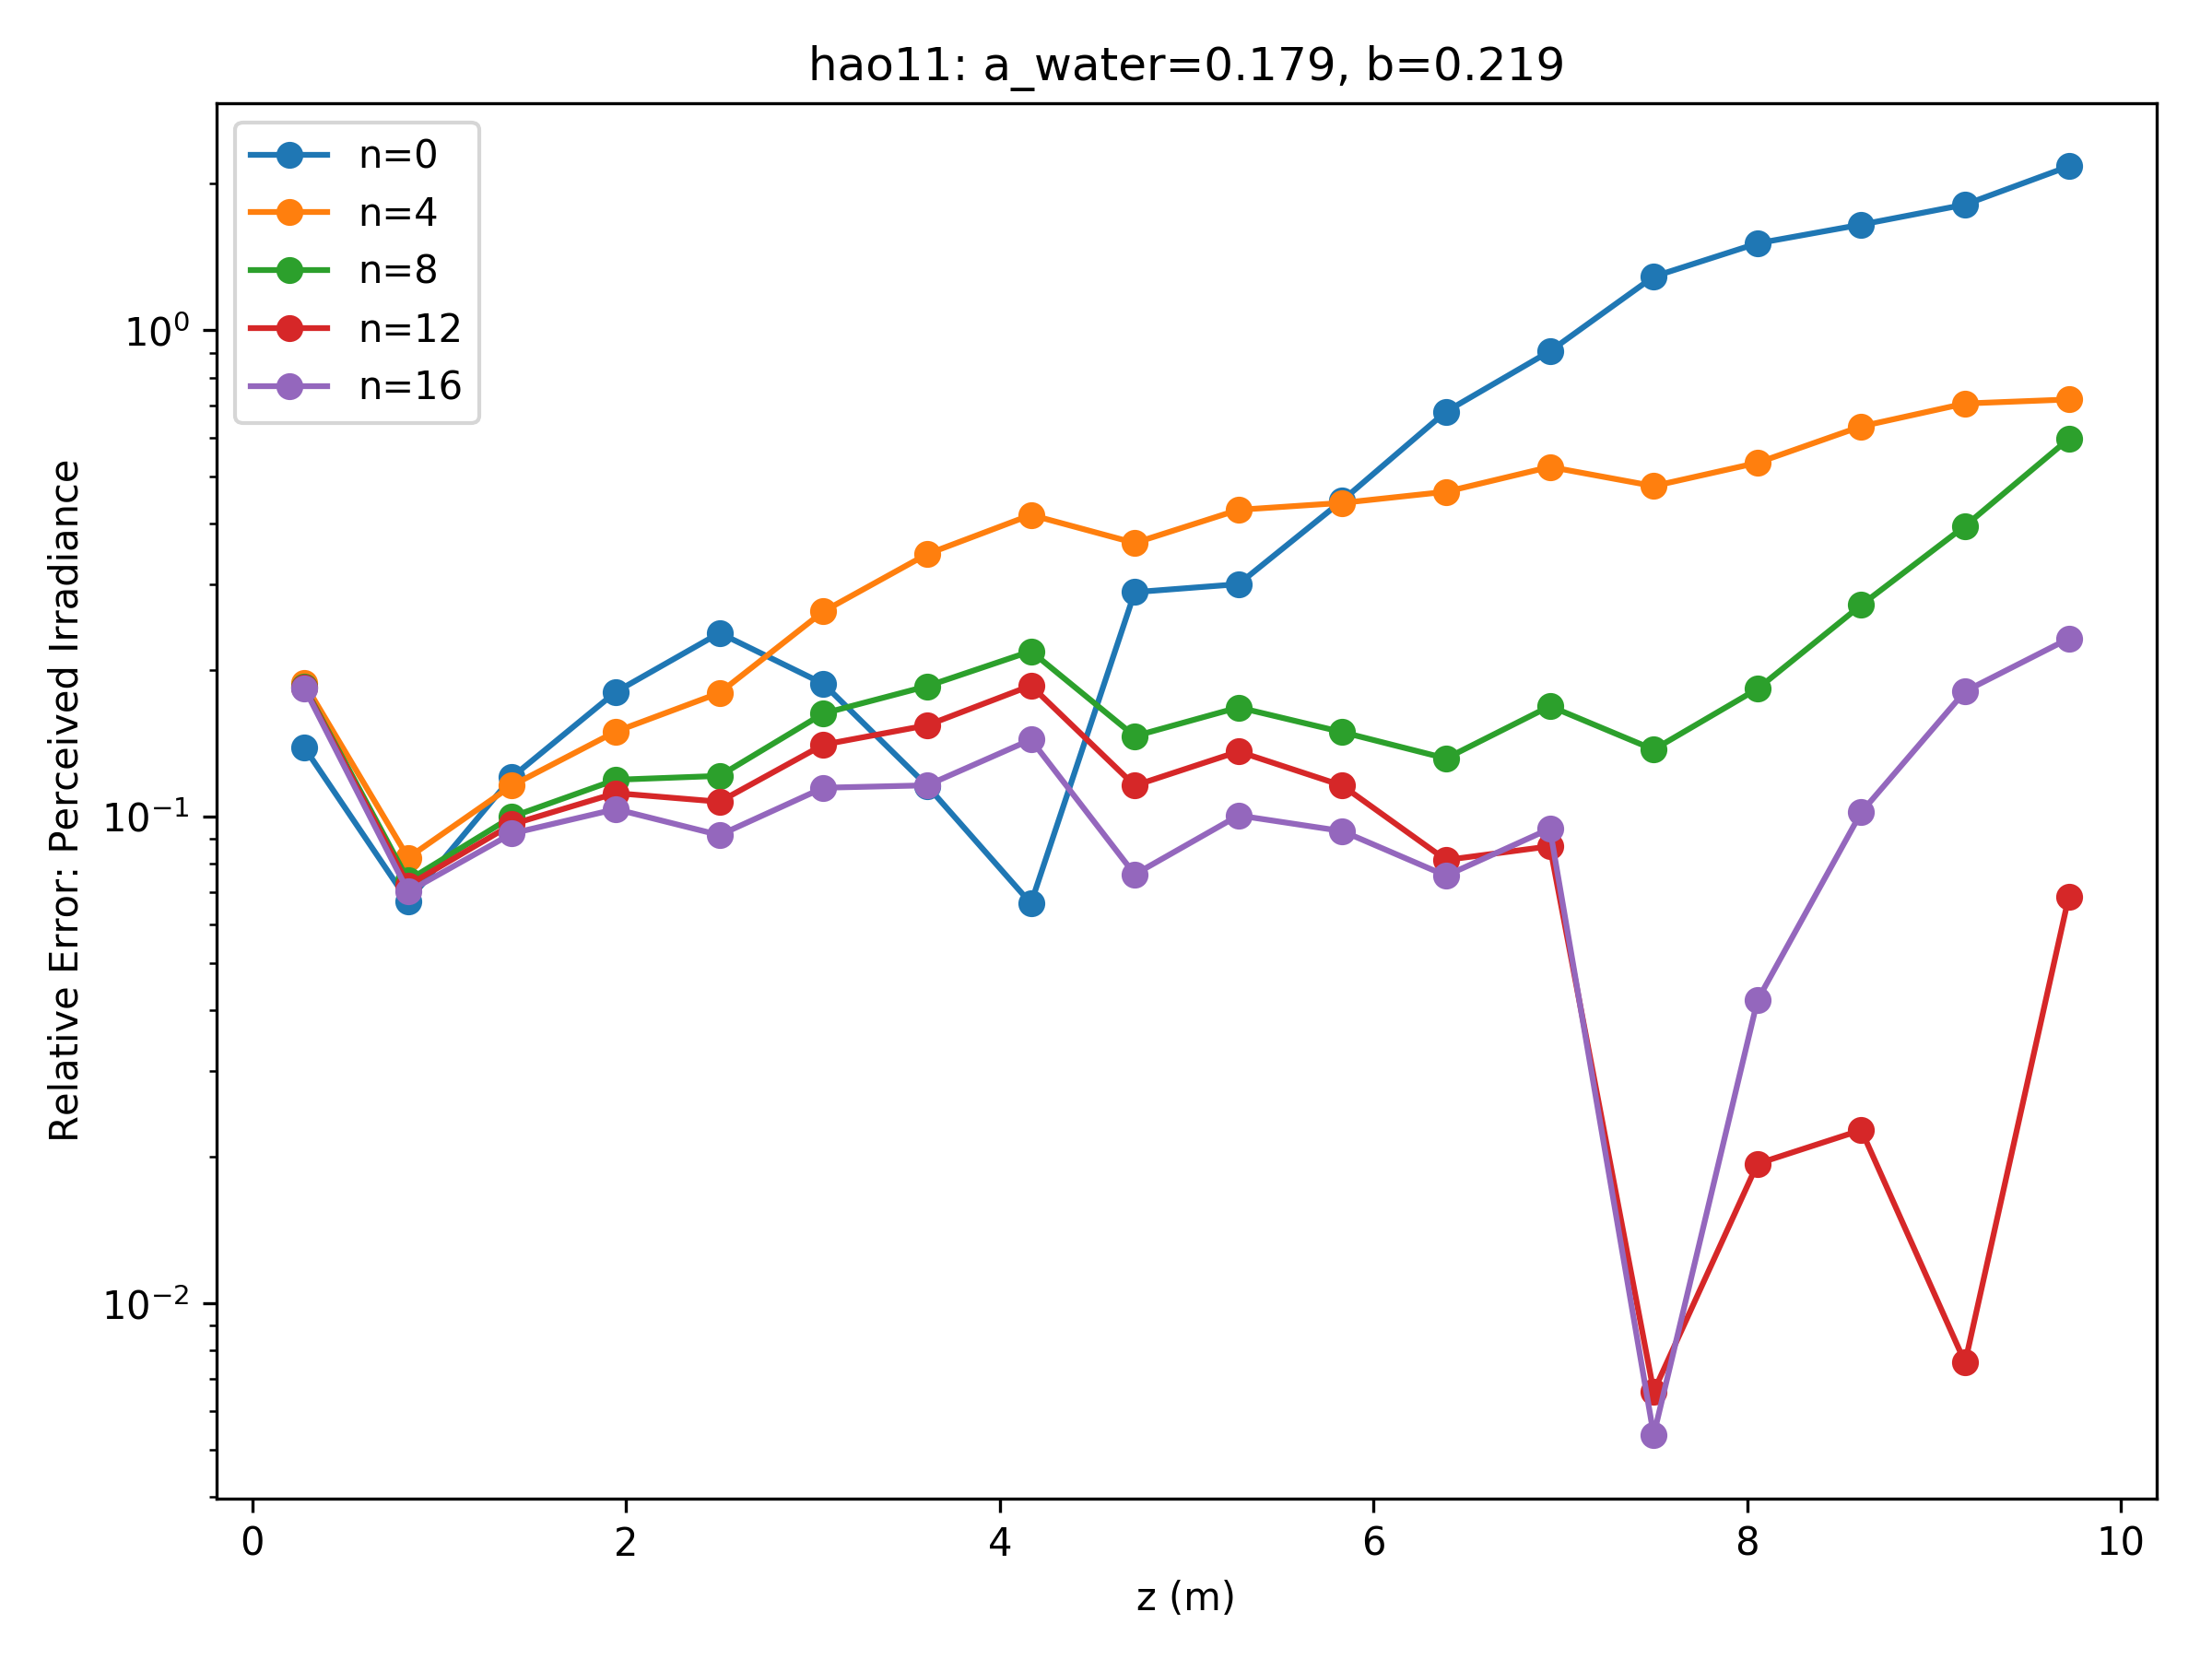
\includegraphics[width=4in]{asym_conv_rel_err_hao11}
  \caption{\DIFaddFL{Successive asymptotic approximations, relative error: }\texttt{\DIFaddFL{HAO11}}}
\end{figure}
\DIFaddend 


\DIFdelbegin \DIFdel{Run Ole Jacob's modelwith my new light model, compare:
}\DIFdelend \DIFaddbegin \begin{figure}[H]
  \centering
  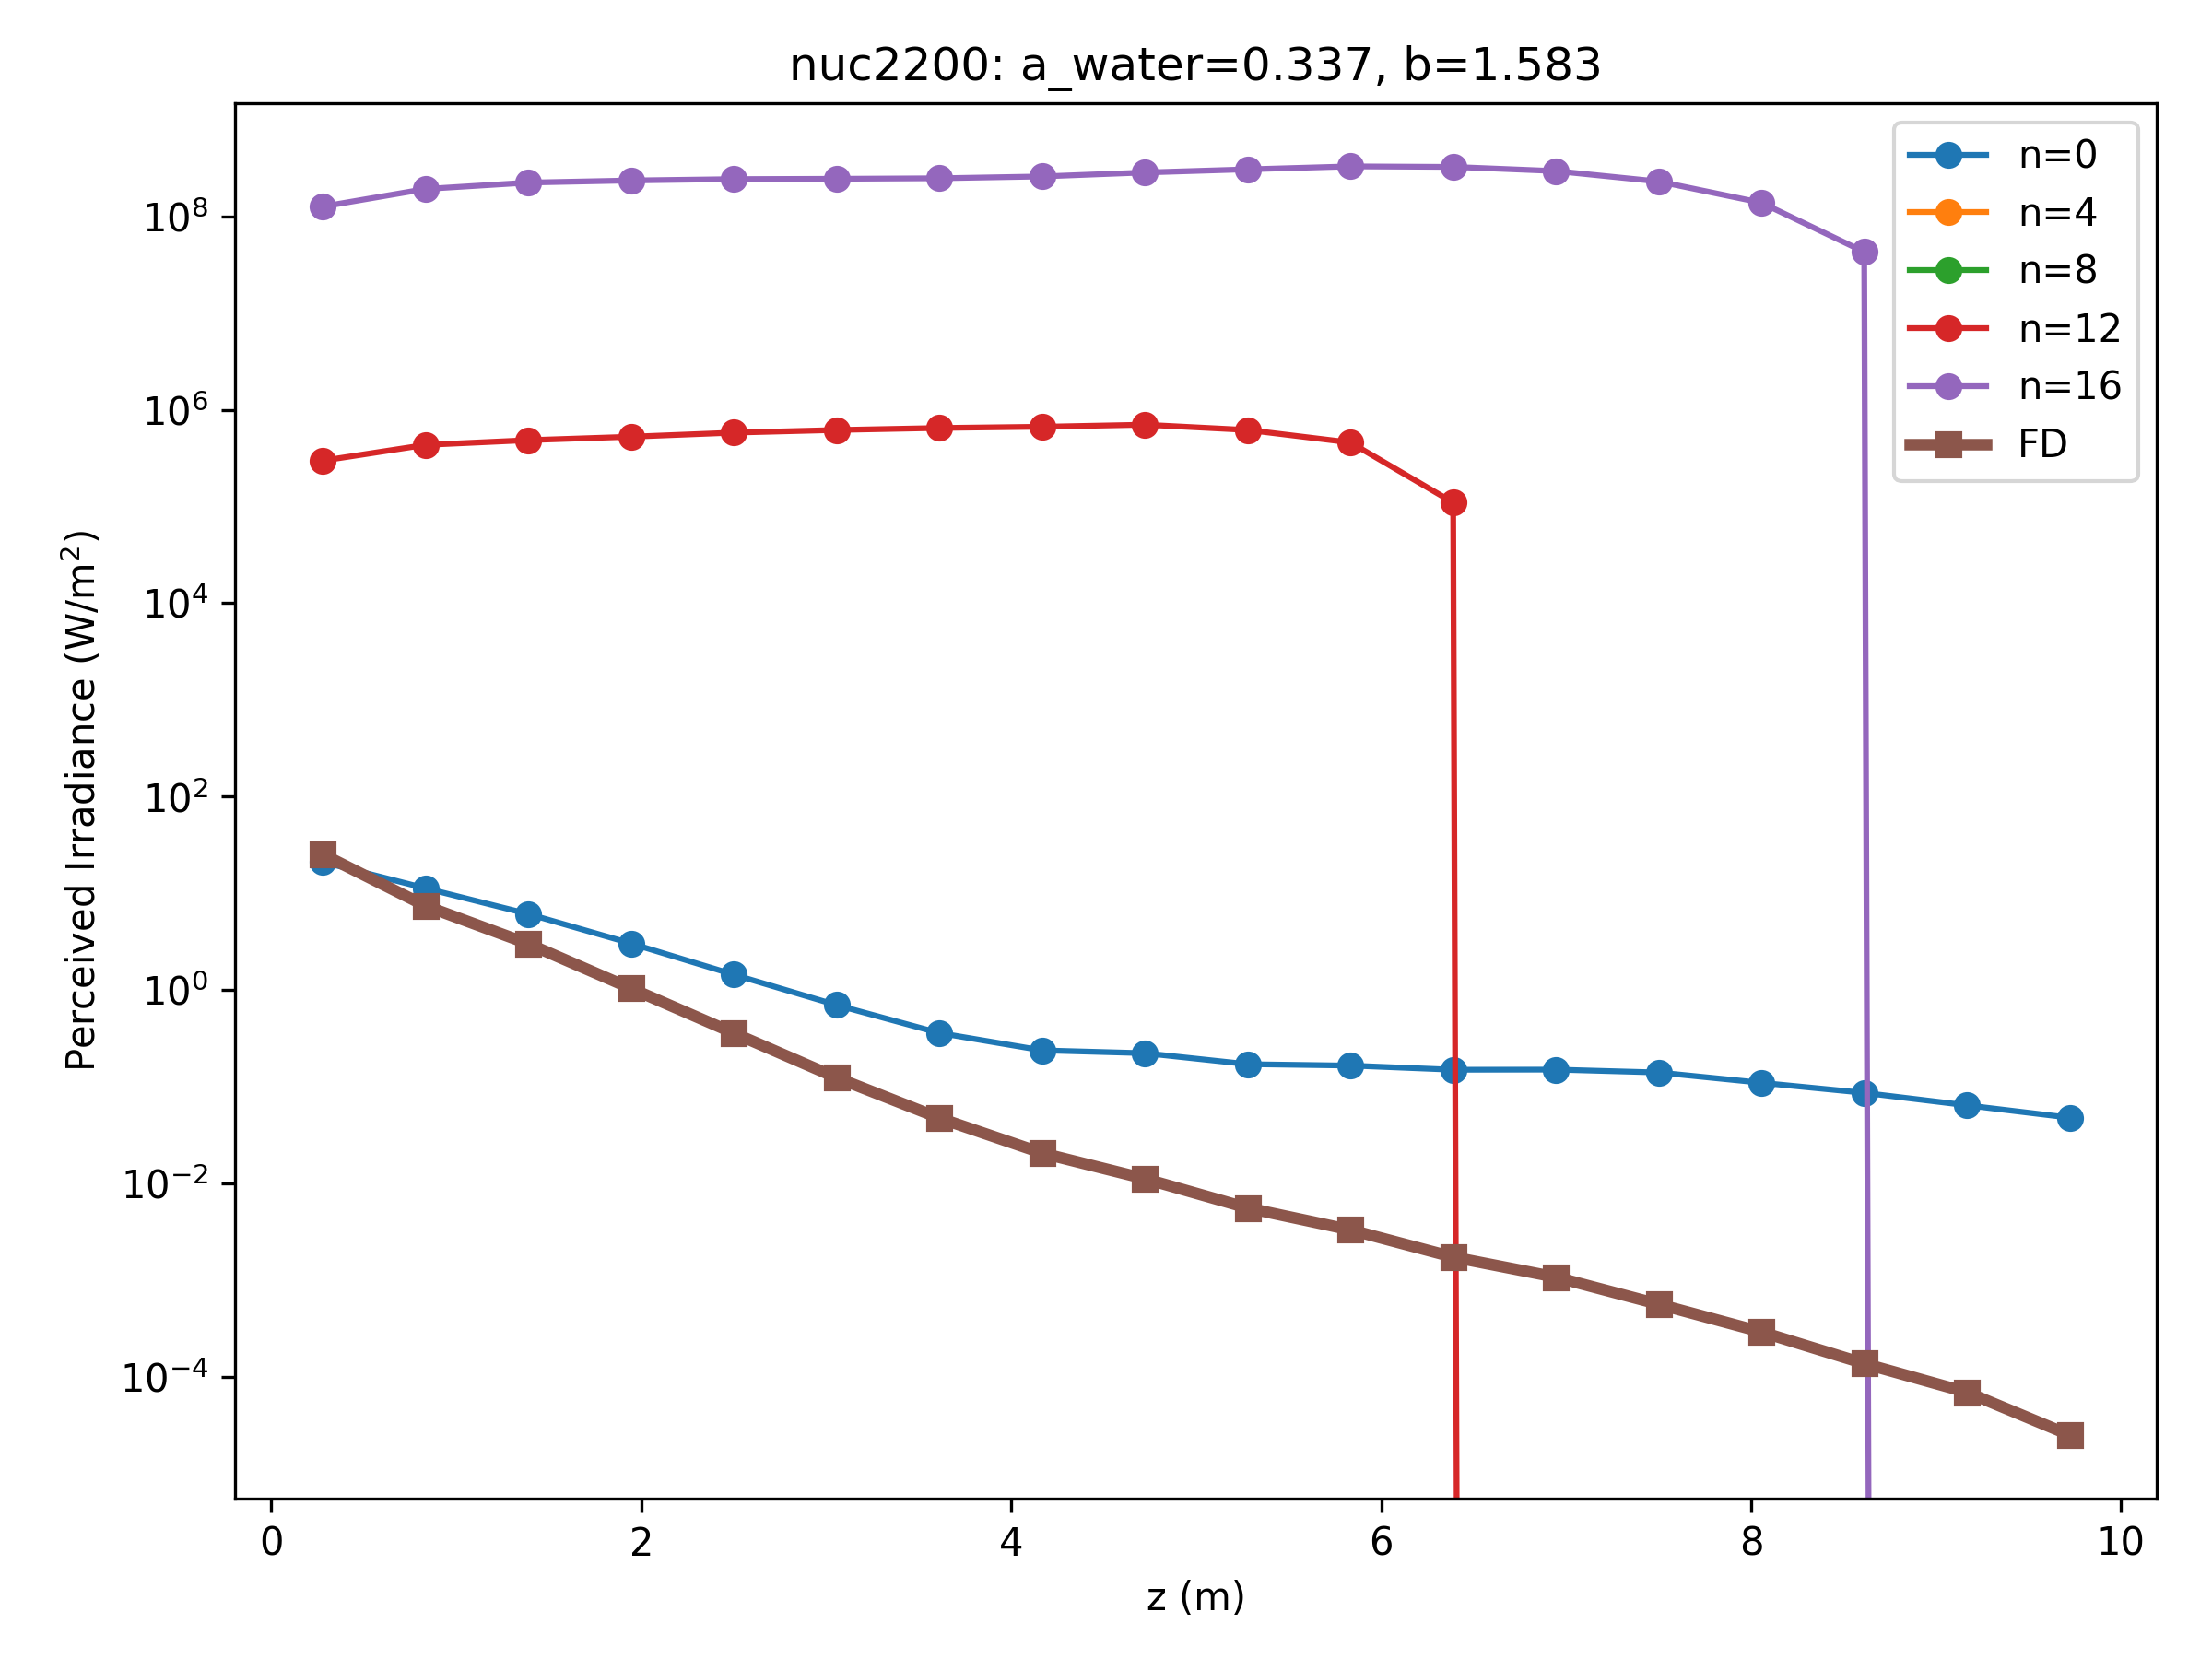
\includegraphics[width=4in]{asym_conv_irrad_nuc2200}
  \caption{\DIFaddFL{Successive asymptotic approximations, irradiance: }\texttt{\DIFaddFL{NUC2200}}}
\end{figure}
\DIFaddend 

\DIFdelbegin \DIFdel{- irrad over time for several depths
}\DIFdelend \DIFaddbegin \begin{figure}[H]
  \centering
  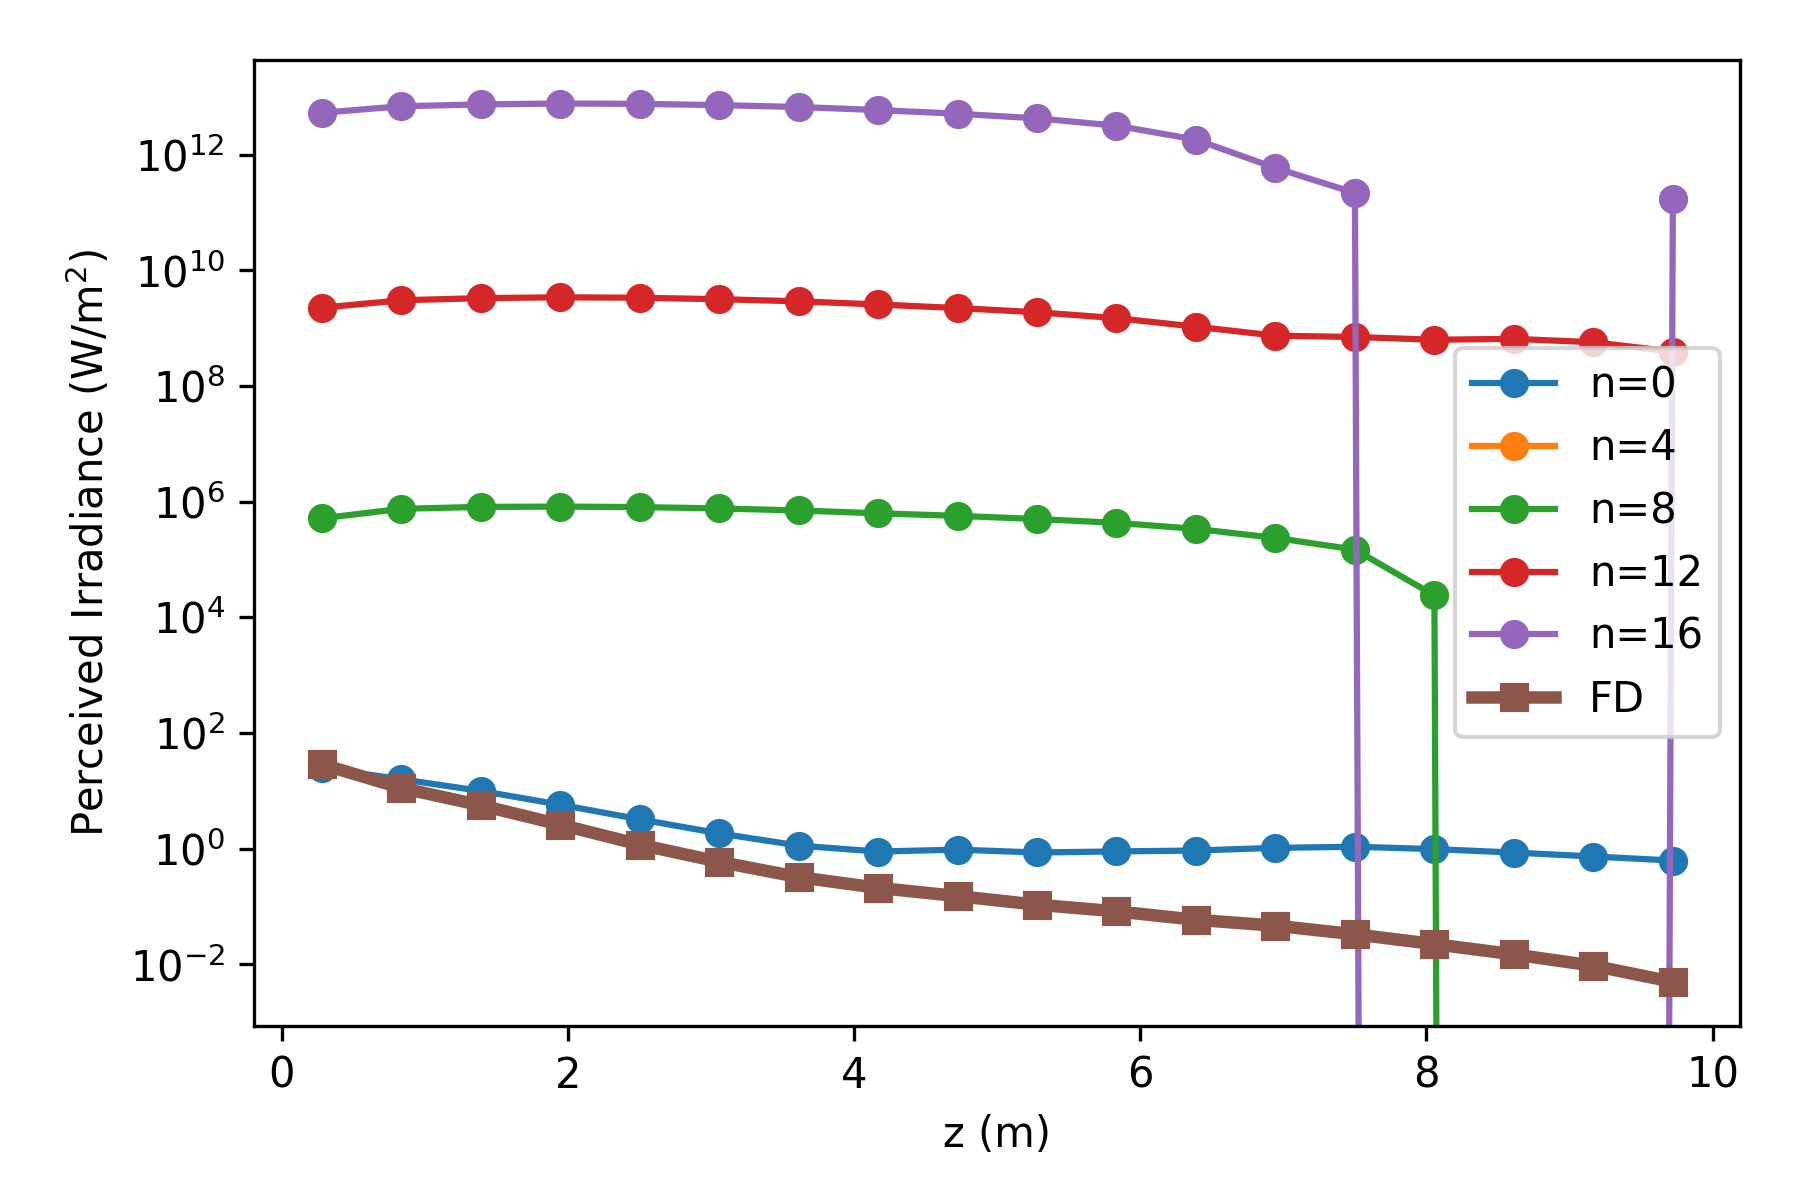
\includegraphics[width=4in]{asym_conv_irrad_nuc2240}
  \caption{\DIFaddFL{Successive asymptotic approximations, relative error: }\texttt{\DIFaddFL{NUC2240}}}
\end{figure}
\DIFaddend 


\DIFdelbegin \DIFdel{- computation time
}\DIFdelend \DIFaddbegin \begin{figure}[H]
  \centering
  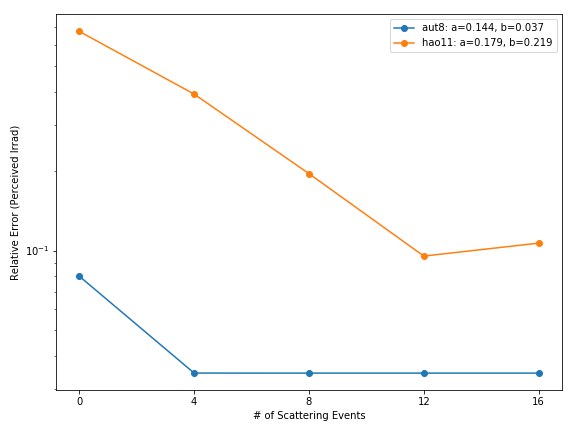
\includegraphics[width=4in]{asym_conv_compare}
  \caption{\DIFaddFL{Comparison of asymptotic approximations for various waters.}}
  \label{fig:asym_conv_compare}
\end{figure}
\DIFaddend 

\DIFdelbegin \DIFdel{- harvestable biomass
 }\DIFdelend \DIFaddbegin \section{\DIFadd{Sensitivity Analysis}}
\DIFadd{In this section, we demonstrate the effect of varying some of the parameters of the model.
The 12-term asymptotic approximation is used.
In Figure \ref{fig:sens_analysis_a_water} and Figure \ref{fig:sens_analysis_b}, the solution
is shown to diverge when the ratio $b/a$ is too large, as in Section \ref{sec:asym_conv}.
}

\begin{figure}[H]
  \centering
  \vspace{-3em}
  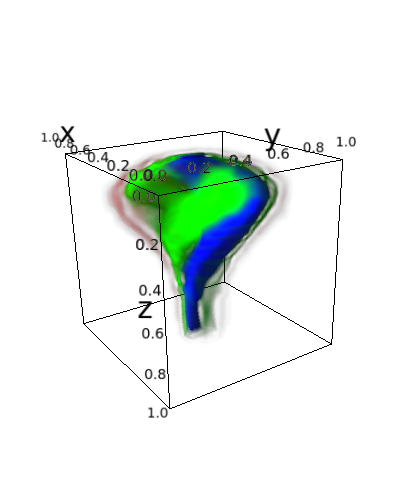
\includegraphics[width=0.45\textwidth]{top-heavy_kelp}
  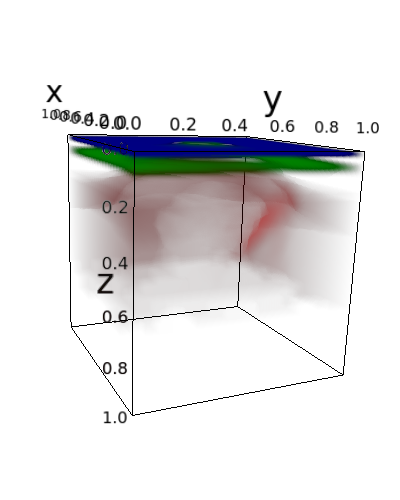
\includegraphics[width=0.45\textwidth]{top-heavy_irrad}
  \caption{\textit{\DIFaddFL{top-heavy}} \DIFaddFL{kelp distribution (left) and no-scattering irradiance profile (right)}}
\end{figure}

\begin{figure}[H]
  \centering
  \vspace{-3em}
  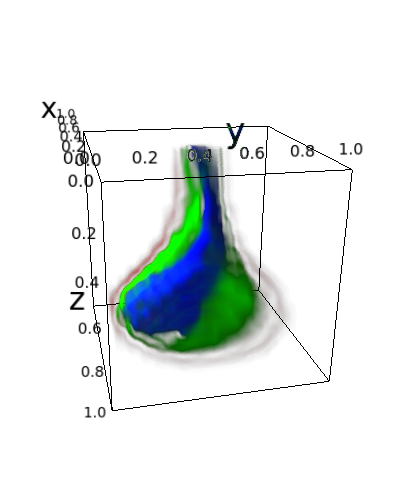
\includegraphics[width=0.45\textwidth]{bottom-heavy_kelp}
  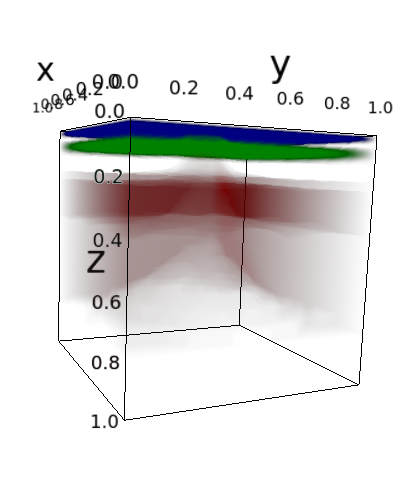
\includegraphics[width=0.45\textwidth]{bottom-heavy_irrad}
  \caption{\textit{\DIFaddFL{bottom-heavy}} \DIFaddFL{kelp distribution (left) and no-scattering irradiance profile (right)}}
\end{figure}

\begin{figure}[H]
  \centering
  \vspace{-3em}
  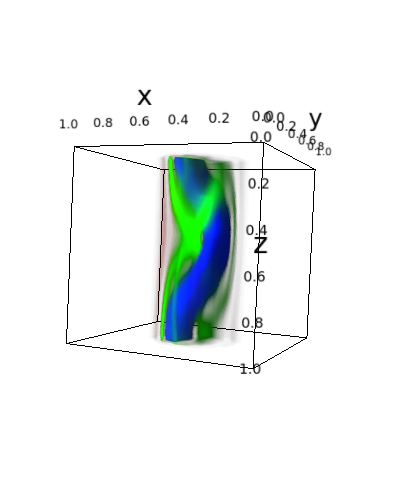
\includegraphics[width=0.45\textwidth]{uniform_kelp}
  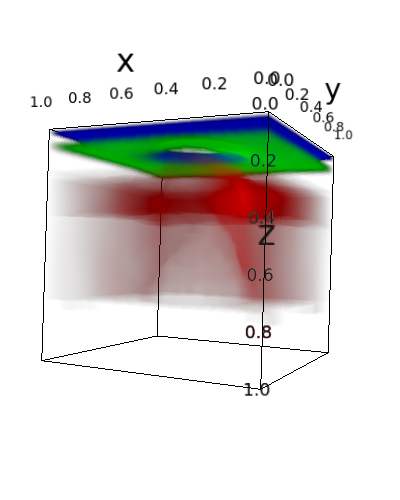
\includegraphics[width=0.45\textwidth]{uniform_irrad}
  \caption{\textit{\DIFaddFL{uniform}} \DIFaddFL{kelp distribution (left) and no-scattering irradiance profile (right)}}
\end{figure}

\begin{figure}[H]
  \centering
  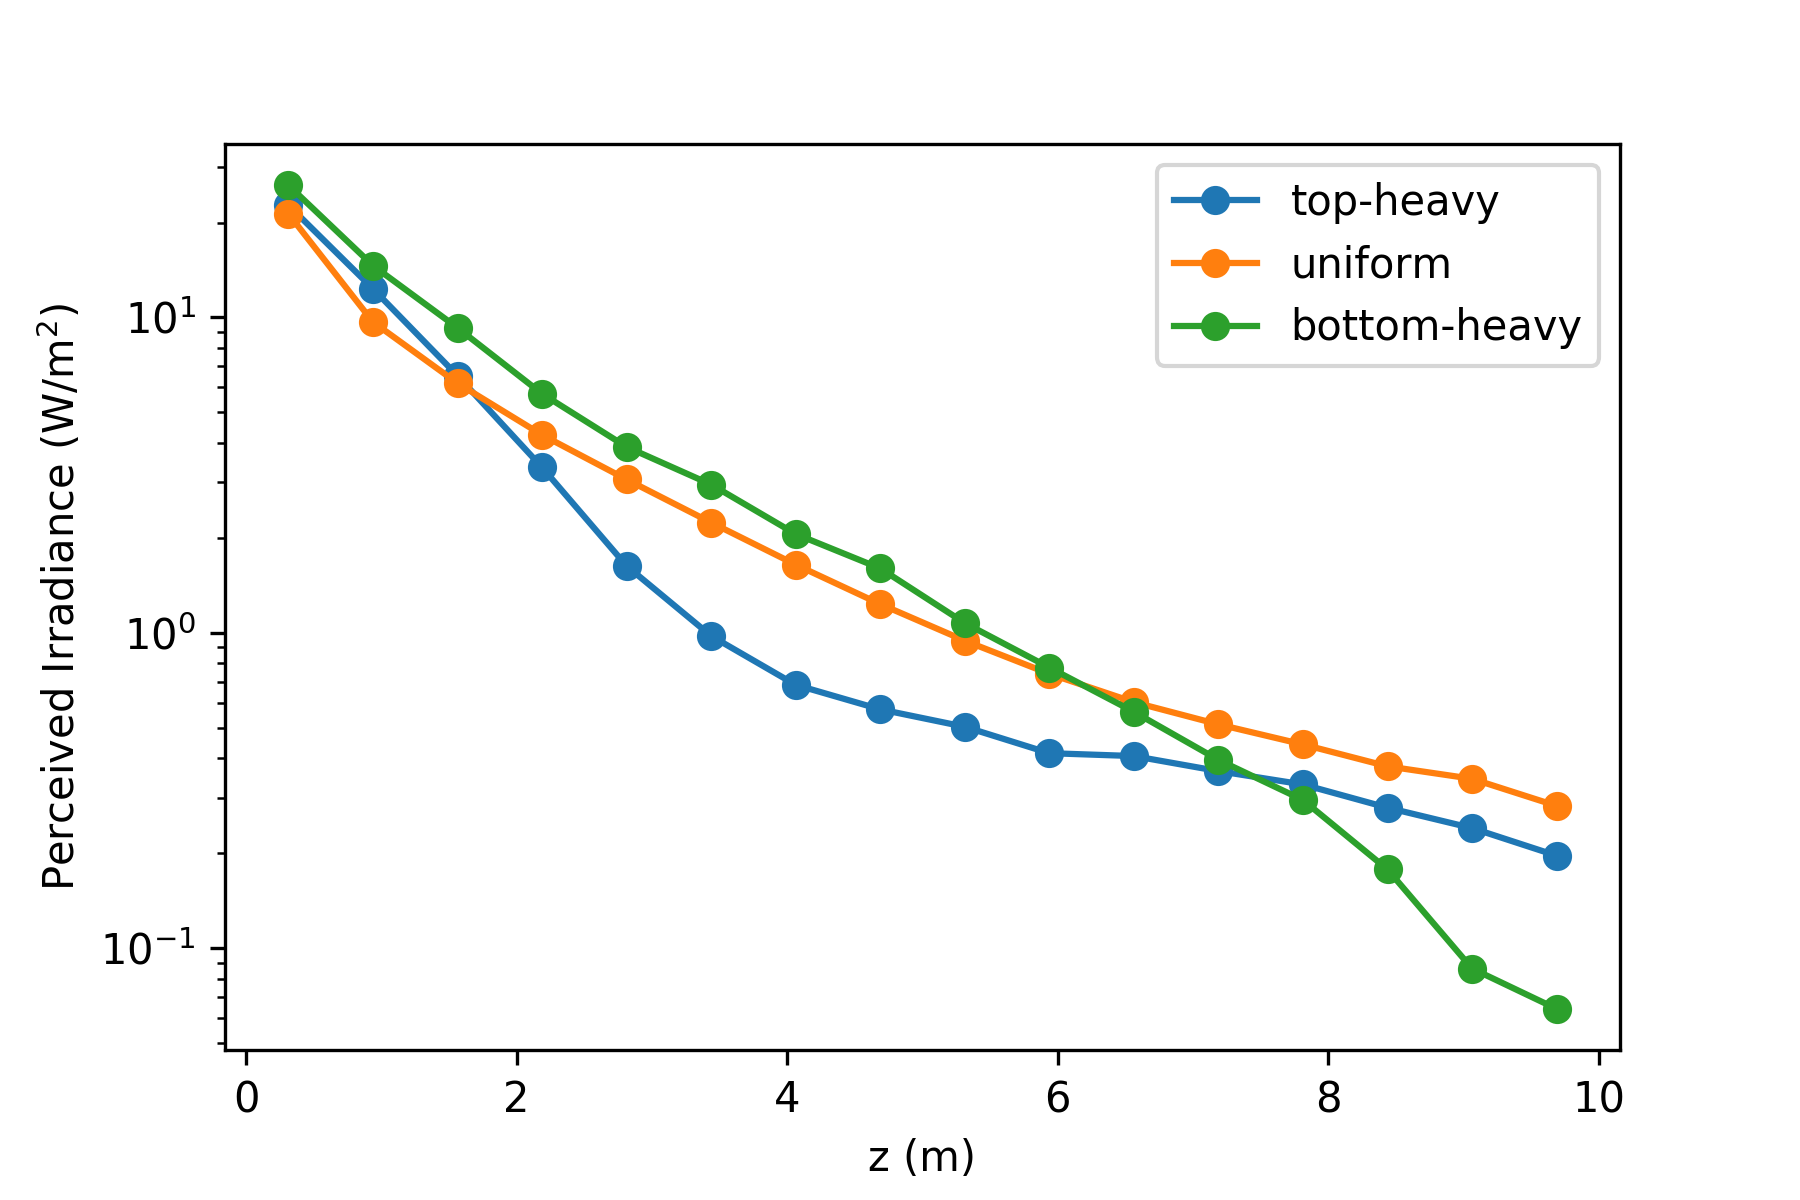
\includegraphics[width=4in]{sens_analysis_kelp_profile}
  \caption{\DIFaddFL{Several kelp profiles}}
\end{figure}

\begin{figure}[H]
  \centering
  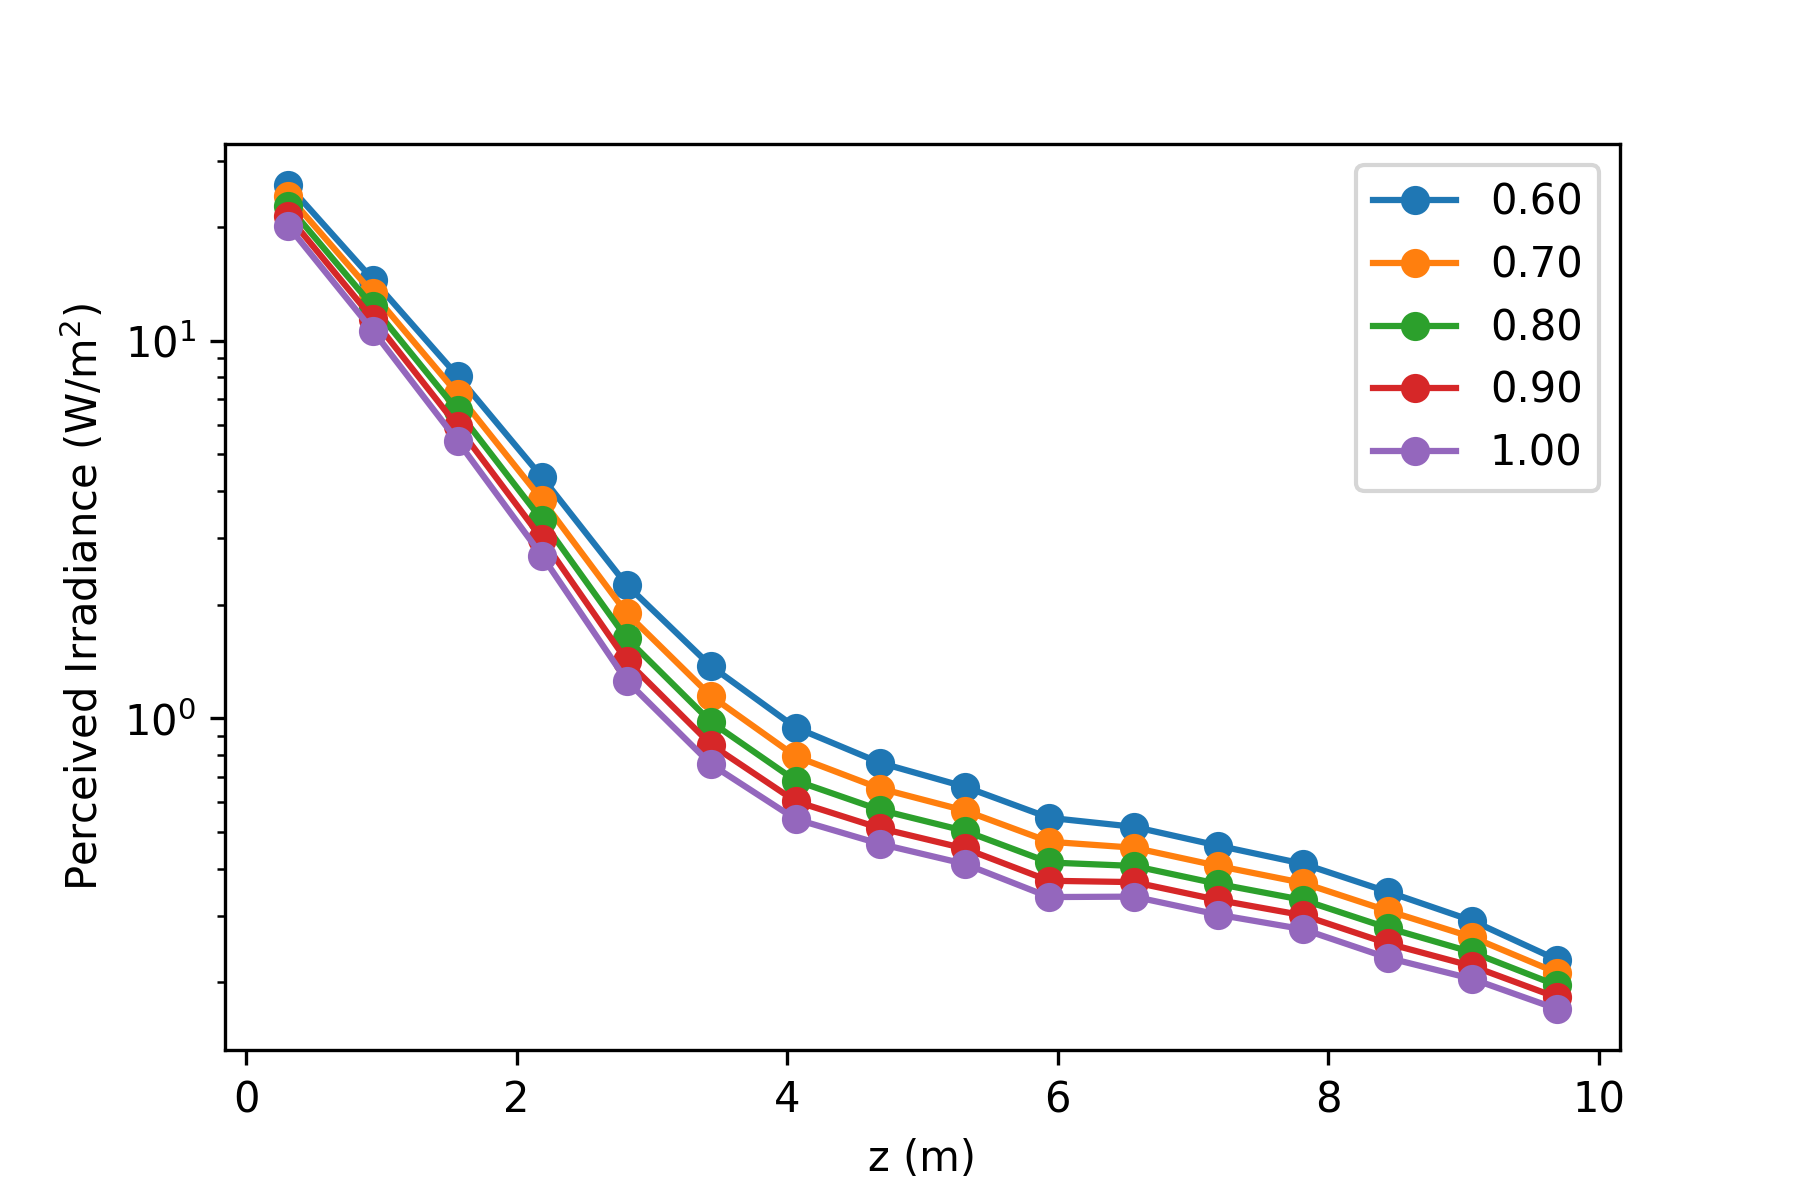
\includegraphics[width=4in]{sens_analysis_absorptance_kelp}
  \caption{\DIFaddFL{Several values of kelp absorptance}}
\end{figure}

\begin{figure}[H]
  \centering
  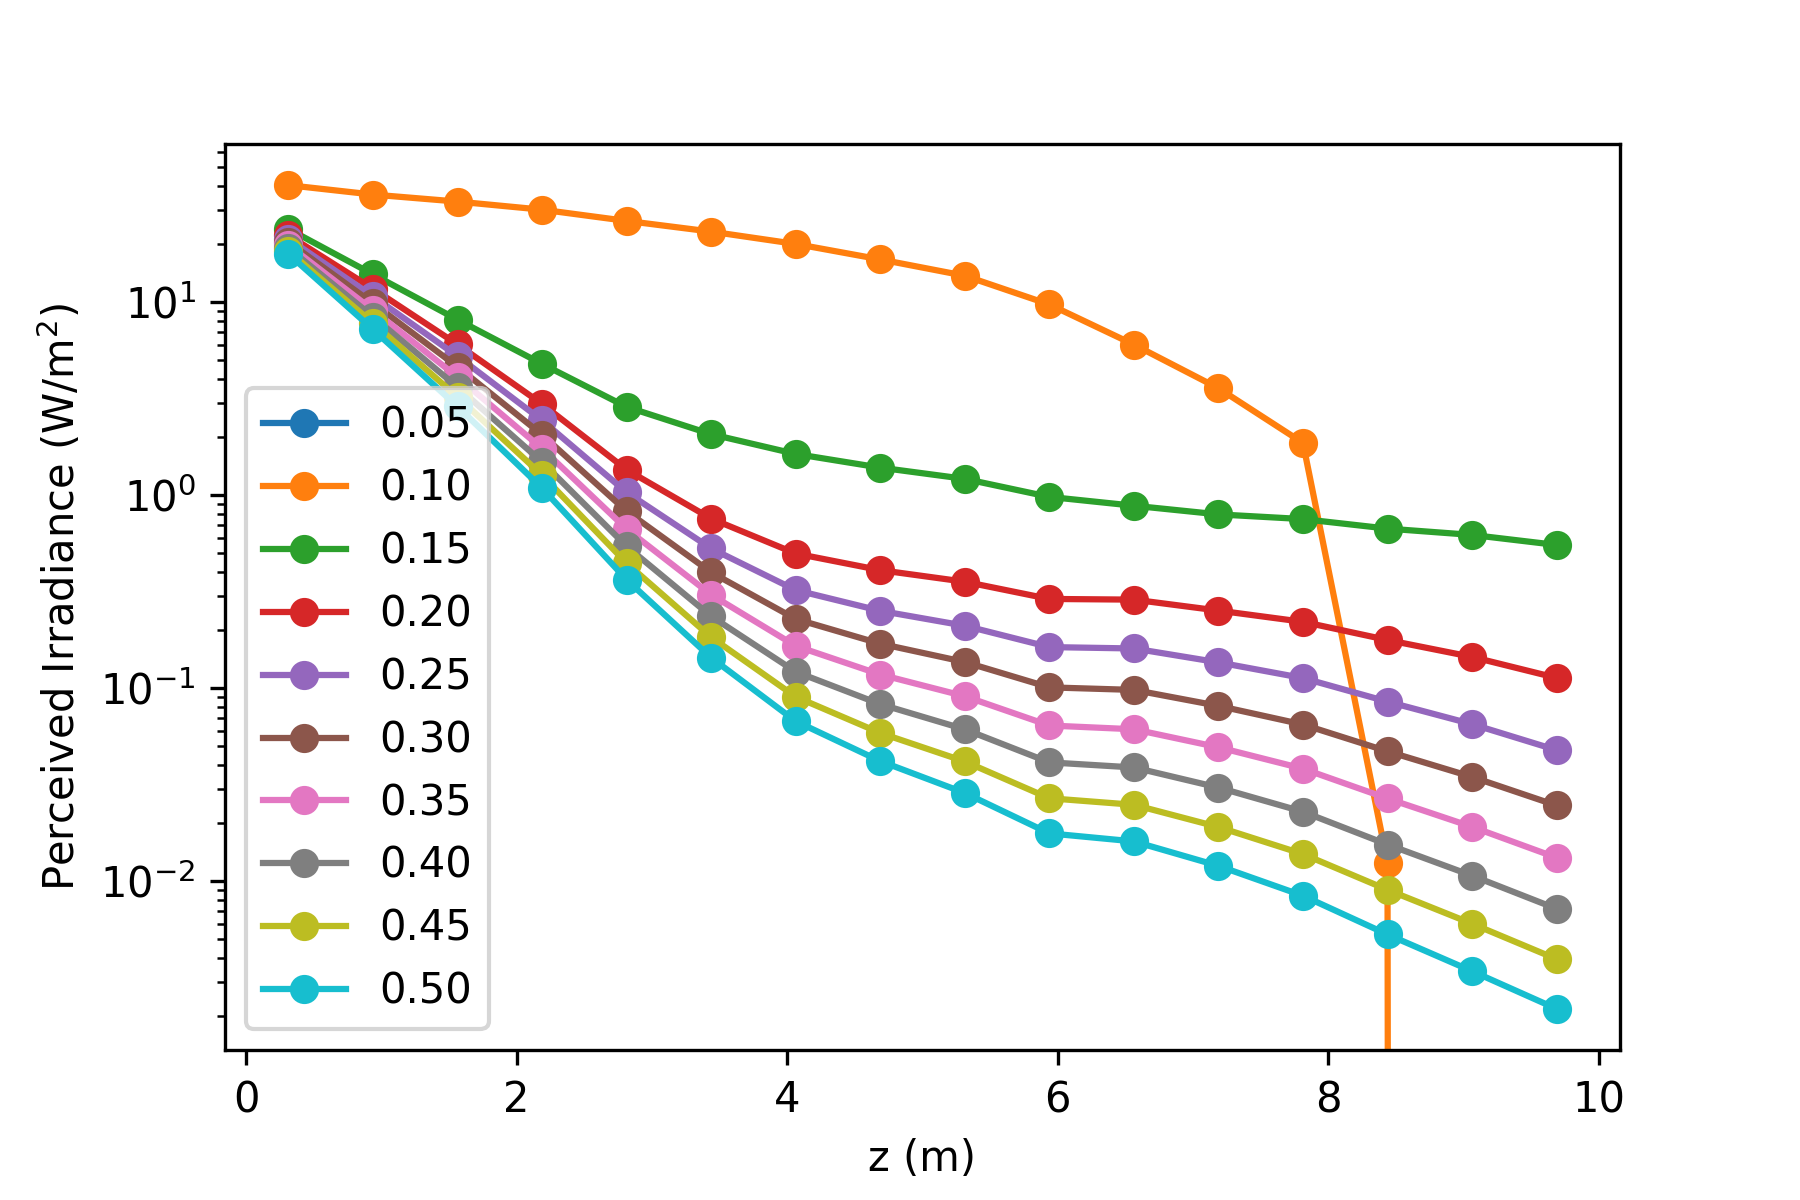
\includegraphics[width=4in]{sens_analysis_a_water}
  \caption{\DIFaddFL{Several values of absorption coefficient of water}}
  \label{fig:sens_analysis_a_water}
\end{figure}

\begin{figure}[H]
  \centering
  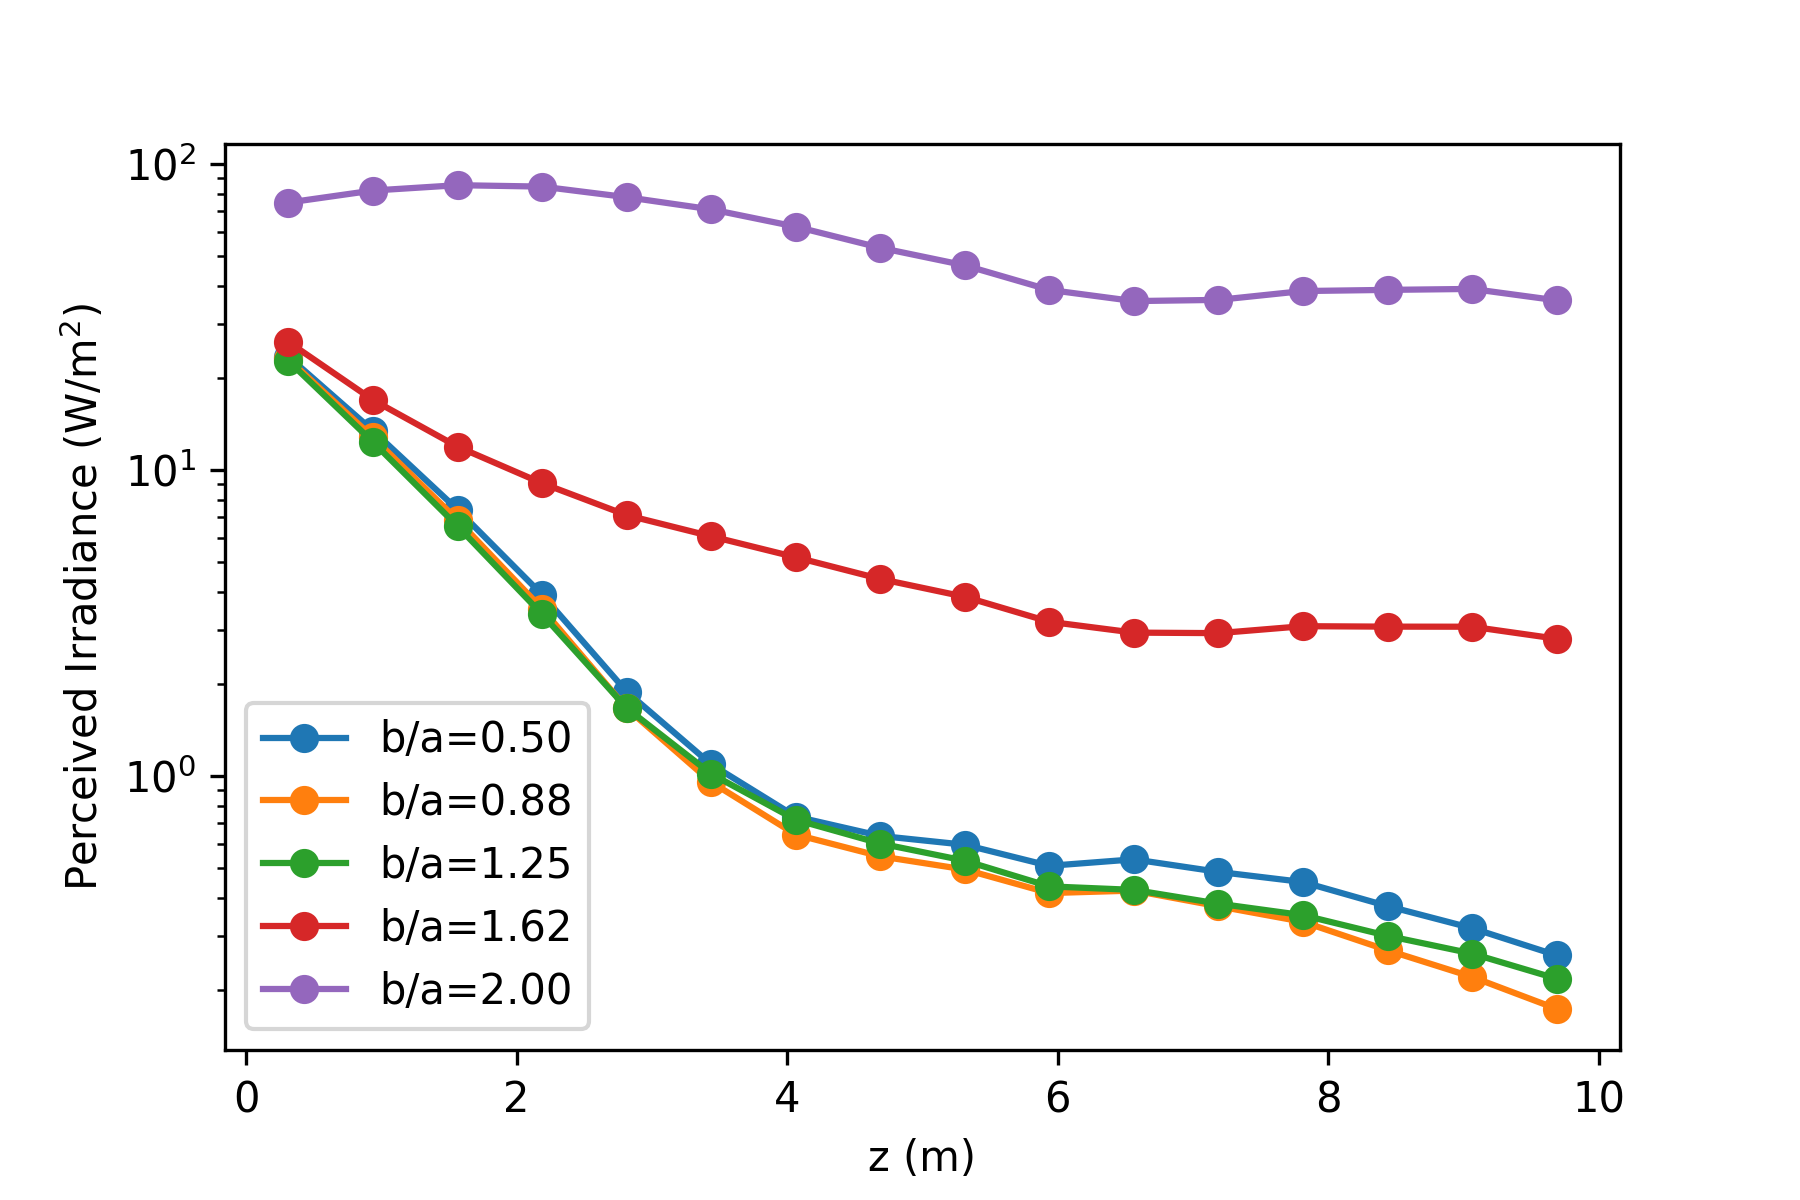
\includegraphics[width=4in]{sens_analysis_b}
  \caption{\DIFaddFL{Several values of scattering coefficient}}
  \label{fig:sens_analysis_b}
\end{figure}
 \DIFaddend \chapter{CONCLUSION}
\label{chap:conclusion}

We present a probabilistic model for the spatial distribution of kelp, and develop a first-principles model for the light field, considering absorption and scattering due to the water and kelp.
A full finite difference solution is presented, and an asymptotic approximation based on discrete scattering events is subsequently developed.
\DIFaddbegin \DIFadd{The asymptotic approximation is shown to converge to the finite difference solution in cases where the absorption coefficient is the same order
of magnitude as the scattering coefficient or larger.
Otherwise, the solution diverges.
}\DIFaddend 

\DIFdelbegin \DIFdel{Future work:
}%DIFDELCMD < \begin{itemize}
\begin{itemize}%DIFAUXCMD
%DIFDELCMD <   \item %%%
\item%DIFAUXCMD
\DIFdel{Frond bending
  }%DIFDELCMD < \item %%%
\item%DIFAUXCMD
\DIFdel{Horizontal kelp ropes (long lines )
  }%DIFDELCMD < \item %%%
\item%DIFAUXCMD
\DIFdel{etc.
}
\end{itemize}%DIFAUXCMD
%DIFDELCMD < \end{itemize}
%DIFDELCMD <  %%%
\DIFdelend \DIFaddbegin \DIFadd{Many aspects of the model have room for future improvement.
The most pressing is probably the development of a model for long-lines, which
is more popular in practice than the vertical lines studied here.
Similar techniques can likely be applied, but the details will of course differ.
}

\DIFadd{One major simplification in the calculation of the kelp model
is the assumption that the fronds are perfectly horizontal.
This could be improved in a straightforward way by including some
probability distribution for the angular elevation as a function of current speed,
similar to the study performed in \mbox{%DIFAUXCMD
\citep{norvik_design_2017}}\hspace{0pt}%DIFAUXCMD
.
The cost of implementing polar rotation is that depth layers are no longer isolated.
Rather than integrating the two dimensional length-orientation distribution from
Section \ref{sec:dist_2d} to calculate the spatial kelp distribution,
it would be necessary to perform a triple integral which includes the elevation distribution.
Since frond elevation and azimuathal orientation are both related to current velocity,
it would likely be impossible to ignore the remarks at the end of \ref{sec:dist_2d}, and the
assumption of independent distributions would have to be abandoned.
}

\DIFadd{Of course, real fronds are not rotating planar kites, but have a very dynamic geometry.
To consider out-of-plane frond bending would require a totally different approach.
Whether or not any improved description of the seaweed would merit the substantial work is unclear.
 }\DIFaddend \bibliographystyle{abbrv}
\bibliography{bio}
\DIFdelbegin %DIFDELCMD < \appendix{2}
%DIFDELCMD < %%%
\DIFdelend \DIFaddbegin \appendix{3}
\chapter{\DIFadd{GRID DETAILS}}
\label{chap:grid_details}

\DIFadd{The width of the spatial grid cells in each dimension are
}\begin{align*}
  \DIFadd{dx }&\DIFadd{= \frac{x_{\max}-x_{\min}}{n_x}, }\\ 
  \DIFadd{dy }&\DIFadd{= \frac{y_{\max}-y_{\min}}{n_y}, }\\ 
  \DIFadd{dz }&\DIFadd{= \frac{z_{\max}-z_{\min}}{n_z}.
}\end{align*}
\DIFadd{Denote the edges as 
}\begin{align*}
  \DIFadd{x_i^e }&\DIFadd{= (i-1)dx \mbox{ for } i=1,\ldots,n_x }\\
  \DIFadd{y_j^e }&\DIFadd{= (j-1)dy \mbox{ for } j=1,\ldots,n_y }\\
  \DIFadd{z_k^e }&\DIFadd{= (k-1)dz \mbox{ for } k=1,\ldots,n_z 
}\end{align*}
\DIFadd{and the cell centers as
}\begin{align*}
  \DIFadd{x_i }&\DIFadd{= (i-1/2)dx \mbox{ for } i=1,\ldots,n_x }\\
  \DIFadd{y_j }&\DIFadd{= (j-1/2)dy \mbox{ for } j=1,\ldots,n_y }\\
  \DIFadd{z_k }&\DIFadd{= (k-1/2)dz \mbox{ for } k=1,\ldots,n_z
}\end{align*}


\DIFadd{Note that in this convention, there are the same number of edges and cells,
and edges precede centers.
}

\DIFadd{Now, we define the azimuthal angle such that
}\begin{align*}
  \DIFadd{\theta_l = (l-1)d\theta.
}\end{align*}
\DIFadd{For the sake of periodicity, we need
}\begin{align*}
  \DIFadd{\theta_1 }&\DIFadd{= 0, }\\
  \DIFadd{\theta_{n_\theta} }&\DIFadd{= 2\pi-d\theta,
}\end{align*}
\DIFadd{which requires
}\begin{equation*}
  \DIFadd{d\theta = \frac{2\pi}{n_\theta}.
}\end{equation*}

\DIFadd{For the polar angle, we similarly let
}\begin{equation*}
  \DIFadd{\phi_m = (m-1)d\phi
}\end{equation*}

\DIFadd{Since the polar azimuthal is not periodic, we also store the endpoint, so
}\begin{align*}
  \DIFadd{\phi_1 }&\DIFadd{= 0, }\\
  \DIFadd{\phi_{n_\phi} }&\DIFadd{= \pi.
}\end{align*}

\DIFadd{This gives us
}\begin{align*}
  \DIFadd{d\phi }&\DIFadd{= \frac{\pi}{n_\phi-1}.
}\end{align*}

\DIFadd{It is also useful to define the edges between angular grid cells as
}\begin{alignat}{\DIFadd{3}}
  \DIFadd{\theta_l^e }&\DIFadd{= (l-1/2) d\theta, }&\DIFadd{\quad l}&\DIFadd{=1,\ldots,n_\theta }\\
  \DIFadd{\phi_m^e }&\DIFadd{= (m-1/2) d\phi, }&\DIFadd{\quad m}&\DIFadd{=1,\ldots,n_\phi-1.
}\end{alignat}

\DIFadd{Note that while $\theta$ has its final edge following its final center, this is
not the case for $\phi$.
}

\begin{figure}[h]
  \centering
  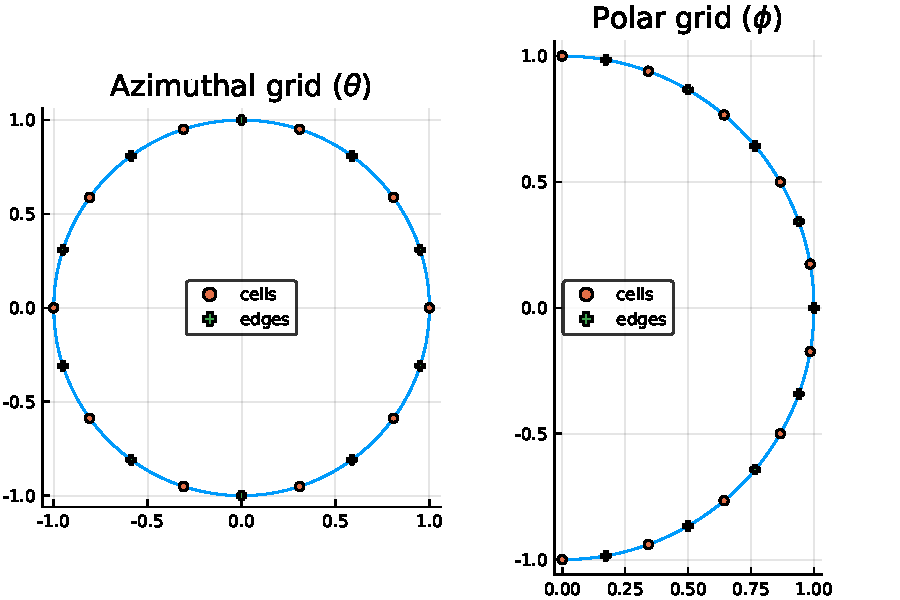
\includegraphics[width=.75\linewidth]{angular_grid_plots}
  \caption{\DIFaddFL{Angular grid}}
\end{figure}

\DIFadd{The following notation is used.
}\begin{align*}
  \DIFadd{\hat{l}(p) }&\DIFadd{= \mbox{mod1}(p, n_\theta) }\\
  \DIFadd{\hat{m}(p) }&\DIFadd{= \ceil(p/n_\theta) + 1 }\\
  \DIFadd{\hat{\theta}_p }&\DIFadd{= \theta_{\hat{l}(p)} }\\
  \DIFadd{\hat{\phi}_p }&\DIFadd{= \phi_{\hat{m}(p)}
}\end{align*}

\DIFadd{Thus, it follows that
}\begin{equation*}
  \DIFadd{p = \left( \hat{m}(p)-2\right)n_\theta + \hat{l}(p).
}\end{equation*}

\DIFadd{Accordingly, define
}\begin{equation*}
  \DIFadd{\hat{p}(l,m) = (m-1)n_\theta + l.
}\end{equation*}

\DIFadd{Further, we refer to the angular grid cell centered at $\vec{\omega}_p$ as $\Omega_p$, and the solid angle subtended by $\Omega_p$ is denoted $\abs{\Omega_p}$.
The areas of the grid cells are calculated as follows.
Note that there is a temporary abuse of notation in that the same symbols ($d\theta$ and $d\phi$) are being used for infinitesimal differential and for finite grid spacing.
}

\DIFadd{For the poles, we have
}\begin{align*}
  \DIFadd{\abs{\Omega_1} = \abs{\Omega_\nomega} }&\DIFadd{= \int_{\Omega_1} d}{\DIFadd{\vec{\omega}}} \\
  &\DIFadd{= \int_0^{2\pi}\int_0^{d\phi/2} \sin\phi\, d\phi\, d\theta }\\
  &\DIFadd{= 2\pi \cos\phi \Big|_{d\phi/2}^0 }\\
  &\DIFadd{= 2\pi(1-\cos(d\phi/2))
}\end{align*}

\DIFadd{And for all other angular grid cells,
}\begin{align*}
  \DIFadd{\abs{\Omega_p} }&\DIFadd{= \int_{\Omega_p} d}{\DIFadd{\vec{\omega}}} \\
                 &\DIFadd{= \int_{\theta_l^e}^{\theta_{l+1}^e}\int_{\phi_m^e}^{\phi_{m+1}^e} \sin(\phi)\, d\phi\, d\theta }\\
                 &\DIFadd{= d\theta \int_{\phi_m^e}^{\phi_{m+1}^e} \sin(\phi)\, d\phi }\\
                 &\DIFadd{= d\theta\left( \cos(\phi_m^e)-\cos(\phi_{m+1}^e) \right).
}\end{align*}

 \DIFaddend \chapter{RAY TRACING ALGORITHM}
\label{chap:ray_tracing}


In order to evaluate a path integral through the previously described grid, it
is first necessary to construct a one-dimensional piecewise constant integrand
which is discontinuous at unevenly spaced points corresponding to the
intersections between the path and edges in the spatial grid.

Consider a grid center $\vec{p_1} = (p_{1x},p_{1y},p_{1z})$ and a corresponding path $\vec{l}(\vec{x_1}, \vec{\omega}, s)$.
To find the location of discontinuities in the itegrand, we first calculate the
distance from its origin, $\vec{p_0} = \vec{x_0}(\vec{p_1}, \vec{\omega}) = (p_{0x}, p_{0y}, p_{0z})$ to grid edges in each dimension
separately.

Given
\begin{align}
  x_i &= p_{0x} + \frac{s_i^x}{\tilde{s}}(p_{1x}-p_{0x}) \\
  y_j &= p_{0y} + \frac{s_j^y}{\tilde{s}}(p_{1y}-p_{0y}) \\
  z_k &= p_{0z} + \frac{s_k^z}{\tilde{s}}(p_{1z}-p_{0z})
\end{align}

we have
\begin{align}
  s_i^x &= \tilde{s}\frac{x_i-p_{0x}}{p_{1x}-p_{0x}} \\
  s_i^y &= \tilde{s}\frac{y_i-p_{0y}}{p_{1y}-p_{0y}} \\
  s_i^z &= \tilde{s}\frac{z_i-p_{0z}}{p_{1z}-p_{0z}} \\
\end{align}


We also keep a record for each dimension specifying whether the ray increases
or decreases in the dimension. Let
\begin{align}
  \delta_x &= \sign(p_{0x}-p_{1x}) \\
  \delta_y &= \sign(p_{0y}-p_{1y}) \\
  \delta_z &= \sign(p_{0z}-p_{1z})
\end{align}

For convenience, we also store a closely related quantity, $\sigma$ with a value 1 for
increasing rays and 0 for decreasing rays in each dimension
\begin{align}
  \sigma_x = (\delta_x+1)/2 \\
  \sigma_y = (\delta_y+1)/2 \\
  \sigma_z = (\delta_z+1)/2
\end{align}

For this algorithm, we keep two sets of indices. $(i,j,k)$ indexes the grid
cell, and will be used for extracting physical quantities from each cell along
the path.
Meanwhile, $(i^e,j^e,k^e)$ will index the edges between grid cells, beginning
after the first cell. i.e., $i^e=1$ refers not to the plane $x=\xmin$, but to $x=\xmin+dx$.

Let $(i_0, j_0, k_0)$ be the indices of the grid cell containing $\vec{p_0}$.

That is,

\begin{align}
  i_0 &= \ceil\left(\frac{p_{0x}-\xmin}{dx}\right) \\
  j_0 &= \ceil\left(\frac{p_{0y}-\ymin}{dy}\right) \\
  k_0 &= \ceil\left(\frac{p_{0z}-\zmin}{dz}\right)
\end{align}

Then,
\begin{align}
  i_0^e &= i_0 + \sigma_x \\
  j_0^e &= j_0 + \sigma_y \\
  k_0^e &= k_0 + \sigma_z
\end{align}

Now, we calculate the distance from $p_0$ along the path to edges in each dimension.
\begin{align}
  s_i^x = \hat{s}\frac{x_i^e-p_{0x}}{p_{1x}-p_{0x}} \\
  s_j^y = \hat{s}\frac{y_j^e-p_{0y}}{p_{1y}-p_{0y}} \\
  s_k^z = \hat{s}\frac{z_k^e-p_{0z}}{p_{1z}-p_{0z}}
\end{align}

For each grid cell, we check the path lengths required to cross the next $x$, $y$, and
$z$ edge-planes.
Then, we move to the next grid cell in that dimension.
That is,

* We also track $s$, the path length.

Consider $i,j,k$ fixed (denoting the current grid cell).

\begin{align}  
  d = \mbox{argmin}_{x,y,z} \left\{ s_i^x-s, s_j^y-s, s_k^z \right\}
\end{align}

* This doesn't quite make sense yet.
\begin{align}
  \begin{cases}
    i = i+\delta_x, & \mbox{if } d=x \\
    j = j+\delta_y, & \mbox{if } d=y \\
    z = k+\delta_z, & \mbox{if } d=z
  \end{cases}
\end{align}

and

\begin{align}
  \begin{cases}
    i^e = i^e+\delta_x, & \mbox{if } d=x \\
    j^e = j^e+\delta_y, & \mbox{if } d=y \\
    z^e = k^e+\delta_z, & \mbox{if } d=z
  \end{cases}
\end{align}


Then, move to the adjacent grid cell in the dimension which requires the shortest
step to reach an edge. Save $ds$ of the path through this cell. Also save abs.
coef. and source.
 \chapter{FORTRAN CODE}
\label{chap:fortran}

The full FORTRAN implementation of the model described in this thesis.
This code can be found online at:

\begin{verbatim}
https://github.com/OliverEvans96/kelp
https://gitlab.com/OliverEvans96/kelp
\end{verbatim}

utils.f90
\lstinputlisting{utils.f90}

sag.f90
\lstinputlisting{sag.f90}

kelp3d.f90
\lstinputlisting{kelp3d.f90}

rte\_sparse\_matrices.f90
\lstinputlisting{rte_sparse_matrices.f90}

rte3d.f90
\lstinputlisting{rte3d.f90}

kelp\_context.f90
\lstinputlisting{kelp_context.f90}

light\_context.f90
\lstinputlisting{light_context.f90}

asymptotics.f90
\lstinputlisting{asymptotics.f90}

light\_interface.f90
\lstinputlisting{light_interface.f90}

 \end{document}
